% ==================================================================
%  徐森林、薛春华《数学分析》（第二册）
%  第 8 章  n 元函数微分学
% ==================================================================

\chapter{\texorpdfstring{$n$}{n} 元函数微分学}\label{ch:8}

本章引进方向导数与偏导数, 并用偏导数表达方向导数; 给出了复合函数的求导链规则. 作为它的应用, 证明在区域 $U$ 上, 如果 $\left.\dfrac{\partial f}{\partial x_{i}}\right|_{U} \equiv 0\ (i = 1, 2, \cdots, n)$, $f$ 在 $\overline{U}$ 上连续, 则 $f$ 为常值函数. 接着详细讨论了函数可微与映射可微的重要概念, 得到了可微的充分条件和必要条件, 以及函数的高维微分中值定理与映射的拟微分中值定理. $n$ 元 Lagrange 型余项的 Taylor 公式与 Peano 型余项的 Taylor 公式是 $n$ 元微分学的重要定理. Peano 型余项 Taylor 公式的惟一性定理保证了用各种方法 Taylor 展开的合法性. Lagrange 型余项的 Taylor 公式在第 9 章极值研究中起到重要作用. 最后, 隐射 (隐函数) 与逆映 (反函数) 定理的两种精美的证明, 使读者得到了分析能力的严格训练. 这些知识在第 9 章参数曲面与条件极值研究中有重要应用.

% ==================================================================
%  §8.1  方向导数与偏导数
%  源：徐森林、薛春华《数学分析》第二册，印刷页 54-69 (PDF p. 60-75)
%  底本：PaddleOCR-VL-1.6 JSON/MD 识别结果，人工逐字核校与公式精修
%  规范：全西文标点，忠实原文定义、注、定理、例题、练习题编号与推导
% ==================================================================

\section{方向导数与偏导数}\label{sec:8.1}

对一元函数 $y = f(x)$, 如果极限
\[
  \lim_{t \to 0}\frac{f(x_{0} + t) - f(x_{0})}{t} = \lim_{\Delta x \to 0}\frac{f(x_{0} + \Delta x) - f(x_{0})}{\Delta x} = \lim_{x \to x_{0}}\frac{f(x) - f(x_{0})}{x - x_{0}}
\]
存在有限, 则 $f$ 在 $x_{0}$ 处可导, 且上述极限就是 $f$ 在 $x_{0}$ 处的导数 $f'(x_{0}) = \dfrac{\mathrm{d}f}{\mathrm{d}x}\Big|_{x = x_{0}} = \dfrac{\mathrm{d}y}{\mathrm{d}x}\Big|_{x = x_{0}} = y'(x_{0})$, 它是 $f$ 在 $x_{0}$ 处的变化率.

$f$ 在 $x_{0}$ 处可导 $\iff f$ 在 $x_{0}$ 处的左、右导数相等, 即
\[
  f_{-}'(x_{0}) = \lim_{x \to x_{0}^{-}}\frac{f(x) - f(x_{0})}{x - x_{0}} = \lim_{x \to x_{0}^{+}}\frac{f(x) - f(x_{0})}{x - x_{0}} = f_{+}'(x_{0}).
\]

在 $\mathbb{R}^{n}\ (n \geqslant 2)$ 中, 一个点的开邻域中过该点不只是两个方向, 而是有无穷多个方向. 因此, 代替左、右导数应考虑方向导数.

\begin{definition}\label{def:8.1.1}
设 $U \subset \mathbb{R}^{n}$ 为开集 (今后都指 Euclid 空间 $(\mathbb{R}^{n}, \mathcal{T}_{\rho_{0}}^{n})$ 中的开集), $f: U \to \mathbb{R}^{1}$, $\boldsymbol{e}$ 为 $\mathbb{R}^{n}$ 中的一个单位向量, $\boldsymbol{x}^{0} \in U$, 令
\[
  u(t) = f(\boldsymbol{x}^{0} + t\boldsymbol{e})
\]
(此时 $u$ 为 $t$ 的一元函数). 如果 $u$ 在 $t = 0$ 的导数
\[
  u'(0) = \lim_{t \to 0}\frac{u(t) - u(0)}{t} = \lim_{t \to 0}\frac{f(\boldsymbol{x}^{0} + t\boldsymbol{e}) - f(\boldsymbol{x}^{0})}{t}
\]
存在有限, 则称它为 $f$ 在点 $\boldsymbol{x}^{0}$ 沿方向 $\boldsymbol{e}$ 的\textbf{方向导数}, 记作 $\dfrac{\partial f}{\partial \boldsymbol{e}}(\boldsymbol{x}^{0})$, 它就是 $f$ 在点 $\boldsymbol{x}^{0}$ 沿方向 $\boldsymbol{e}$ 的变化率 (\cref{fig:8.1.1}), 且 $\tan\theta = \dfrac{\partial f}{\partial \boldsymbol{e}}(\boldsymbol{x}^{0})$.
\end{definition}

\begin{figure}[htbp]
  \centering
  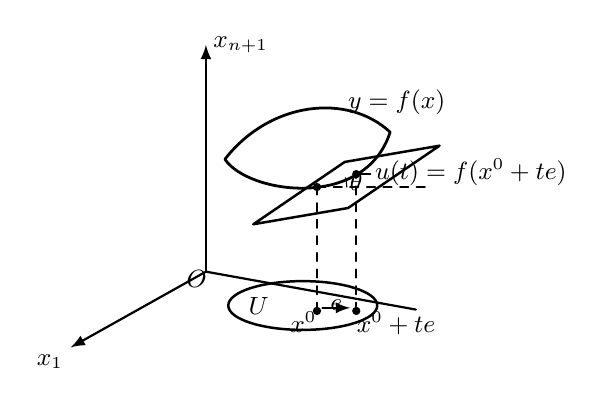
\begin{tikzpicture}[x=0.86cm, y=0.86cm, >=latex, line cap=round, line join=round]
    % ---------- 坐标架 ----------
    \draw[line width=0.8pt, ->] (0, 0) -- (-2.00, -1.12) node[below left=-1pt] {\small $x_{1}$};
    \draw[line width=0.8pt, ->] (0, 0) -- (0, 3.35) node[right=-1pt] {\small $x_{n+1}$};
    \draw[line width=0.8pt] (0, 0) -- (3.10, -0.56);
    \node[below left=-1.5pt, inner sep=1pt] at (0, 0) {\small $O$};
    % ---------- 底面区域 U ----------
    \draw[line width=0.9pt] (1.43, -0.50) ellipse (1.10 and 0.36);
    \node[inner sep=1pt] at (0.78, -0.50) {\small $U$};
    \fill (1.64, -0.58) circle (1.5pt);
    \node[below left=-1.5pt, inner sep=1.5pt] at (1.64, -0.58) {\small $x^{0}$};
    \fill (2.22, -0.58) circle (1.5pt);
    \node[below right=-1.5pt, inner sep=1.5pt] at (2.22, -0.58) {\small $x^{0}+te$};
    \draw[->, line width=0.8pt] (1.72, -0.535) -- (2.13, -0.535);
    \node[above=-2pt, inner sep=1pt] at (1.925, -0.54) {\small $e$};
    % ---------- 竖直虚线与曲面片 ----------
    \draw[line width=0.7pt, dashed] (1.64, -0.58) -- (1.64, 1.25);
    \draw[line width=0.7pt, dashed] (2.22, -0.58) -- (2.22, 1.44);
    % 曲面片 y = f(x)：「透镜」轮廓（下缘经过 A、B）
    \draw[line width=1.0pt]
      (0.28, 1.66)
      .. controls (0.95, 2.52) and (2.10, 2.64) .. (2.72, 2.06)
      .. controls (2.35, 0.90) and (0.62, 1.15) .. (0.28, 1.66);
    \node[anchor=west, inner sep=1pt] at (2.05, 2.50) {\small $y = f(\boldsymbol{x})$};
    % 曲面上的点 A(x^0) 与 B(x^0+te)
    \fill (1.64, 1.25) circle (1.5pt);
    \fill (2.22, 1.44) circle (1.5pt);
    \node[anchor=west, inner sep=1pt] at (2.45, 1.47) {\small $u(t) = f(\boldsymbol{x}^{0} + t\boldsymbol{e})$};
    \draw[line width=0.5pt] (2.43, 1.44) -- (2.24, 1.44);
    % 平面（由 e 方向与竖直方向张成的平行四边形）
    \draw[line width=0.9pt] (0.70, 0.70) -- (2.10, 0.94) -- (3.45, 1.86) -- (2.05, 1.62) -- cycle;
    % 过 A 的水平虚线 与 夹角 theta
    \draw[line width=0.7pt, dashed] (1.64, 1.25) -- (3.25, 1.25);
    \draw (2.08, 1.25) arc[start angle=0, end angle=18.1, radius=0.44];
    \node[inner sep=1pt] at (2.22, 1.33) {\small $\theta$};
  \end{tikzpicture}
  \caption{}\label{fig:8.1.1}
\end{figure}

\begin{example}\label{ex:8.1.1}
设 $\boldsymbol{e}$ 为一个方向, 则 $\|-\boldsymbol{e}\| = \|\boldsymbol{e}\| = 1$, 可见 $-\boldsymbol{e}$ 也为一个方向. 此时, 我们有
\begin{align*}
  \frac{\partial f}{\partial(-\boldsymbol{e})}(\boldsymbol{x}^{0})
  &= \lim_{t \to 0}\frac{f(\boldsymbol{x}^{0} + t(-\boldsymbol{e})) - f(\boldsymbol{x}^{0})}{t}
   = -\lim_{-t \to 0}\frac{f(\boldsymbol{x}^{0} + (-t)\boldsymbol{e}) - f(\boldsymbol{x}^{0})}{-t} \\
  &= -\frac{\partial f}{\partial \boldsymbol{e}}(\boldsymbol{x}^{0}).
\end{align*}
\end{example}

\begin{example}\label{ex:8.1.2}
考察二元函数
\[
  f(x, y) = \begin{cases}
    \dfrac{2xy}{x^{2} + y^{2}}, & (x, y) \neq (0, 0), \\[2.5mm]
    1, & (x, y) = (0, 0).
  \end{cases}
\]
记方向 $\boldsymbol{e} = (\cos\theta, \sin\theta)$, $0 \leqslant \theta < 2\pi$, 并取 $\boldsymbol{x}^{0} = (0, 0)$, 当 $t \neq 0$ 时有
\[
  \frac{f(\boldsymbol{x}^{0} + t\boldsymbol{e}) - f(\boldsymbol{x}^{0})}{t} = \frac{f(t\cos\theta, t\sin\theta) - f(0, 0)}{t} = \frac{2\cos\theta\sin\theta - 1}{t} = \frac{\sin 2\theta - 1}{t}.
\]
由此看出, 当且仅当 $\theta = \dfrac{\pi}{4}$ 与 $\dfrac{5\pi}{4}$, 方向导数存在且为零. 而对其他 $\theta$, 方向导数不存在.
\[
  \begin{aligned}
    \frac{\partial f}{\partial \boldsymbol{e}}(\boldsymbol{x}^{0})
    &= \lim_{t \to 0}\frac{f(\boldsymbol{x}^{0} + t\boldsymbol{e}) - f(\boldsymbol{x}^{0})}{t} = \lim_{t \to 0}\frac{\sin 2\theta - 1}{t} \\
    &= \begin{cases}
         0, & \theta = \dfrac{\pi}{4}\ \text{与}\ \dfrac{5\pi}{4}, \\[3.5mm]
         \infty, & \theta \in \left[0, \dfrac{\pi}{4}\right) \bigcup \left(\dfrac{\pi}{4}, \dfrac{5\pi}{4}\right) \bigcup \left(\dfrac{5\pi}{4}, 2\pi\right).
       \end{cases}
  \end{aligned} \qedhere
\]
\end{example}

记 $\boldsymbol{e}_{i} = (0, 0, \cdots, 0, \underset{\text{第 } i \text{ 个}}{1}, 0, \cdots, 0)$ 为 $\mathbb{R}^{n}$ 中的规范正交基, 即
\[
  \langle \boldsymbol{e}_{i}, \boldsymbol{e}_{j} \rangle = \delta_{ij} = \begin{cases} 1, & i = j, \\ 0, & i \neq j. \end{cases}
\]
设 $\boldsymbol{x}^{0} = (x_{1}^{0}, x_{2}^{0}, \cdots, x_{n}^{0})$, 则
\[
  \begin{aligned}
    \frac{\partial f}{\partial \boldsymbol{e}_{i}}(\boldsymbol{x}^{0})
    &= \lim_{t \to 0}\frac{f(\boldsymbol{x}^{0} + t\boldsymbol{e}_{i}) - f(\boldsymbol{x}^{0})}{t} \\
    &= \lim_{t \to 0}\frac{f(x_{1}^{0}, x_{2}^{0}, \cdots, x_{i-1}^{0}, x_{i}^{0} + t, x_{i+1}^{0}, \cdots, x_{n}^{0}) - f(x_{1}^{0}, x_{2}^{0}, \cdots, x_{n}^{0})}{t} \\
    &= \lim_{x_{i} \to x_{i}^{0}}\frac{f(x_{1}^{0}, x_{2}^{0}, \cdots, x_{i-1}^{0}, x_{i}, x_{i+1}^{0}, \cdots, x_{n}^{0}) - f(x_{1}^{0}, x_{2}^{0}, \cdots, x_{n}^{0})}{x_{i} - x_{i}^{0}} \\
    &\reason{记作} \frac{\partial f}{\partial x_{i}}(\boldsymbol{x}^{0}) = f_{x_{i}}'(\boldsymbol{x}^{0}) = f_{i}'(\boldsymbol{x}^{0}),
  \end{aligned}
\]
称它为 $f$ 的第 $i$ 个\textbf{一阶偏导数}, 它是 $\boldsymbol{x}^{0}$ 点处沿 $\boldsymbol{e}_{i}$ 方向的方向导数.

\begin{example}\label{ex:8.1.3}
在 $\mathbb{R}^{n}$ 中计算函数 $f(\boldsymbol{x}) = \|\boldsymbol{x}\| = \sqrt{x_{1}^{2} + x_{2}^{2} + \cdots + x_{n}^{2}}$ 的偏导数, 其中 $\boldsymbol{x} = (x_{1}, x_{2}, \cdots, x_{n})$.

\begin{solution}
当 $\boldsymbol{x} \neq \boldsymbol{0}$ 时,
\[
  f_{x_{i}}'(\boldsymbol{x}) = \frac{1}{2}(x_{1}^{2} + x_{2}^{2} + \cdots + x_{n}^{2})^{-\frac{1}{2}} \cdot 2x_{i} = \frac{x_{i}}{\|\boldsymbol{x}\|}, \quad i = 1, 2, \cdots, n.
\]
当 $\boldsymbol{x} = \boldsymbol{0}$ 时, 设 $\boldsymbol{e}$ 为任一给定的方向 (单位向量), 此时, 极限
\[
  \lim_{t \to 0}\frac{f(t\boldsymbol{e}) - f(\boldsymbol{0})}{t} = \lim_{t \to 0}\frac{\|t\boldsymbol{e}\|}{t} = \lim_{t \to 0}\frac{|t|\,\|\boldsymbol{e}\|}{t} = \lim_{t \to 0}\frac{|t|}{t}
\]
不存在, 即 $f$ 在原点处的任何方向导数都不存在. 特别地, $f$ 在原点处的任何偏导数也不存在.\qedhere
\end{solution}
\end{example}

如果在开集 $U$ 中的每一点有偏导数, 就得到 $n$ 个一阶偏导函数
\[
  \frac{\partial f}{\partial \boldsymbol{e}_{i}} = \frac{\partial f}{\partial x_{i}}, \quad i = 1, 2, \cdots, n.
\]
如果 $f$ 的一阶偏导函数 $\dfrac{\partial f}{\partial x_{i}}$ 又有偏导数, 称为 $f$ 的\textbf{二阶偏导数}, 记作
\[
  f_{x_{i}x_{j}}'' = \frac{\partial^{2}f}{\partial x_{i}\partial x_{j}} = \frac{\partial}{\partial x_{j}}\Big(\frac{\partial f}{\partial x_{i}}\Big),
\]
\[
  f_{x_{i}x_{i}}'' = \frac{\partial^{2}f}{\partial x_{i}^{2}} = \frac{\partial}{\partial x_{i}}\Big(\frac{\partial f}{\partial x_{i}}\Big), \quad i, j = 1, 2, \cdots, n.
\]
类似可定义 $3$ 阶, $4$ 阶, $\cdots$, $m$ 阶, $\cdots$ 偏导数.

$f$ 为 $C^{k}$ 函数, 即

\noindent $k = 0$, $f$ 连续;

\noindent $0 < k < +\infty$, $f$ 在 $U$ 中有直至 $k$ 阶连续偏导数;

\noindent $k = \infty$, $f$ 在 $U$ 中有各阶连续的偏导数;

\noindent $k = \omega$, $f$ 在 $U$ 中是\textbf{实解析}的, 即 $f$ 在 $U$ 中每一点邻近可展开为收敛的 ($n$ 元) 幂级数:
\[
  f(x_{1}, x_{2}, \cdots, x_{n}) = \sum_{k = 0}^{\infty}\sum_{j_{1}, j_{2}, \cdots, j_{k} = 1}^{n} a_{j_{1}j_{2}\cdots j_{k}}(x_{j_{1}}^{0} - x_{j_{1}})(x_{j_{2}}^{0} - x_{j_{2}})\cdots(x_{j_{k}}^{0} - x_{j_{k}}).
\]
记 $C^{k}(U, \mathbb{R}^{1})$ 为从 $U$ 到 $\mathbb{R}^{1}$ 的 $C^{k}$ 函数的全体.

\begin{theorem}\label{thm:8.1.1}
设 $U \subset \mathbb{R}^{2}$ 为开集, $f: U \to \mathbb{R}^{1}$ 为二元函数. 如果 $f_{xy}''$ 与 $f_{yx}''$ 在 $(x_{0}, y_{0}) \in U$ 连续, 则
\[
  f_{xy}''(x_{0}, y_{0}) = f_{yx}''(x_{0}, y_{0}).
\]
\end{theorem}

\begin{proof}
当 $k \neq 0$, $h \neq 0$ 时, 分别对
\[
  \varphi(y) = f(x_{0} + h, y) - f(x_{0}, y)
\]
与
\[
  \psi(x) = f(x, y_{0} + k) - f(x, y_{0})
\]
应用 Lagrange 中值定理, 就有
\begin{align*}
  &\ [f(x_{0} + h, y_{0} + k) - f(x_{0}, y_{0} + k)] - [f(x_{0} + h, y_{0}) - f(x_{0}, y_{0})] \\
  ={} &\ \varphi(y_{0} + k) - \varphi(y_{0}) = \varphi'(y_{0} + \theta_{1}k)k \\
  ={} &\ [f_{y}'(x_{0} + h, y_{0} + \theta_{1}k) - f_{y}'(x_{0}, y_{0} + \theta_{1}k)]k \\
  ={} &\ f_{yx}''(x_{0} + \theta_{2}h, y_{0} + \theta_{1}k)hk, \quad 0 < \theta_{1}, \theta_{2} < 1.
\end{align*}
另一方面
\begin{align*}
  &\ [f(x_{0} + h, y_{0} + k) - f(x_{0}, y_{0} + k)] - [f(x_{0} + h, y_{0}) - f(x_{0}, y_{0})] \\
  ={} &\ [f(x_{0} + h, y_{0} + k) - f(x_{0} + h, y_{0})] - [f(x_{0}, y_{0} + k) - f(x_{0}, y_{0})] \\
  ={} &\ \psi(x_{0} + h) - \psi(x_{0}) = \psi'(x_{0} + \theta_{3}h)h \\
  ={} &\ [f_{x}'(x_{0} + \theta_{3}h, y_{0} + k) - f_{x}'(x_{0} + \theta_{3}h, y_{0})]h \\
  ={} &\ f_{xy}''(x_{0} + \theta_{3}h, y_{0} + \theta_{4}k)hk, \quad 0 < \theta_{3}, \theta_{4} < 1.
\end{align*}
因此
\[
  f_{xy}''(x_{0} + \theta_{3}h, y_{0} + \theta_{4}k) = f_{yx}''(x_{0} + \theta_{2}h, y_{0} + \theta_{1}k).
\]
由于 $f_{xy}''$ 与 $f_{yx}''$ 在 $(x_{0}, y_{0})$ 处连续, 令 $h \to 0$, $k \to 0$ 就得到
\[
  f_{xy}''(x_{0}, y_{0}) = f_{yx}''(x_{0}, y_{0}). \qedhere
\]
\end{proof}

应用\cref{thm:8.1.1}及归纳法立即可得下面定理.

\begin{theoremp}\label{thm:8.1.1p}
$U \subset \mathbb{R}^{n}$ 为开集, $f: U \to \mathbb{R}^{1}$ 为 $n$ 元函数. 如果 $f$ 在 $U$ 上有直至 $k$ 阶的偏导数, 且都在 $\boldsymbol{x}^{0} = (x_{1}^{0}, x_{2}^{0}, \cdots, x_{n}^{0}) \in U$ 连续, 则
\[
  \frac{\partial^{l}f}{\partial x_{i_{1}}\partial x_{i_{2}}\cdots\partial x_{i_{l}}}(\boldsymbol{x}^{0}) = \frac{\partial^{l}f}{\partial x_{i_{2}}\partial x_{i_{1}}\cdots\partial x_{i_{l}}}(\boldsymbol{x}^{0}) = \cdots = \frac{\partial^{l}f}{\partial x_{i_{l}}\partial x_{i_{l-1}}\cdots\partial x_{i_{1}}}(\boldsymbol{x}^{0}),
\]
即任一 $l\ (\leqslant k)$ 阶偏导数与逐次求导的次序无关.
\end{theoremp}

如果\cref{thm:8.1.1}中条件 ``$f_{xy}''$ 与 $f_{yx}''$ 在 $(x_{0}, y_{0})$ 连续'' 不满足, 则其结论 ``$f_{xy}''(x_{0}, y_{0}) = f_{yx}''(x_{0}, y_{0})$'' 不一定成立.

\begin{example}\label{ex:8.1.4}
设
\[
  f(x, y) = \begin{cases}
    xy\dfrac{x^{2} - y^{2}}{x^{2} + y^{2}}, & (x, y) \neq (0, 0), \\[2.5mm]
    0, & (x, y) = (0, 0),
  \end{cases}
\]
则有
\[
  f_{x}'(0, 0) = \lim_{x \to 0}\frac{f(x, 0) - f(0, 0)}{x - 0} = \lim_{x \to 0}\frac{0 - 0}{x} = \lim_{x \to 0}0 = 0,
\]
\[
  f_{y}'(0, 0) = \lim_{y \to 0}\frac{f(0, y) - f(0, 0)}{y - 0} = \lim_{y \to 0}\frac{0 - 0}{y} = \lim_{y \to 0}0 = 0.
\]
当 $(x, y) \neq (0, 0)$ 时,
\[
  f_{x}'(x, y) = y\left[\frac{x^{2} - y^{2}}{x^{2} + y^{2}} + \frac{4x^{2}y^{2}}{(x^{2} + y^{2})^{2}}\right],
\]
\[
  f_{y}'(x, y) = x\left[\frac{x^{2} - y^{2}}{x^{2} + y^{2}} - \frac{4x^{2}y^{2}}{(x^{2} + y^{2})^{2}}\right].
\]
于是, $\forall y$, $f_{x}'(0, y) = -y$, $f_{xy}''(0, 0) = -1$; $\forall x$, $f_{y}'(x, 0) = x$, $f_{yx}''(0, 0) = 1$,
\[
  f_{xy}''(0, 0) \neq f_{yx}''(0, 0).
\]
由此与\cref{thm:8.1.1}可知, $f_{xy}''$ 与 $f_{yx}''$ 在 $(0, 0)$ 至少有一个不连续.
\end{example}

\begin{example}\label{ex:8.1.5}
设 $f(x, y) = xy$, 求 $f$ 在点 $\boldsymbol{x}^{0} = (1, 1)$ 沿方向 $\boldsymbol{e} = \left(\dfrac{1}{\sqrt{2}}, \dfrac{1}{\sqrt{2}}\right)$ 的方向导数.

\begin{solution}[解法 1]
\[
  \frac{f(\boldsymbol{x}^{0} + t\boldsymbol{e}) - f(\boldsymbol{x}^{0})}{t} = \frac{f\left(1 + \dfrac{t}{\sqrt{2}}, 1 + \dfrac{t}{\sqrt{2}}\right) - f(1, 1)}{t} = \frac{\left(1 + \dfrac{t}{\sqrt{2}}\right)^{2} - 1^{2}}{t} = \sqrt{2} + \frac{t}{2},
\]
\[
  \frac{\partial f}{\partial \boldsymbol{e}}(1, 1) = \lim_{t \to 0}\left(\sqrt{2} + \frac{t}{2}\right) = \sqrt{2}.
\]
\end{solution}

\begin{solution}[解法 2]
\begin{align*}
  \frac{\partial f}{\partial \boldsymbol{e}}(1, 1)
  &= \lim_{t \to 0}\frac{f(\boldsymbol{x}^{0} + t\boldsymbol{e}) - f(\boldsymbol{x}^{0})}{t} \\
  &\reason{\cref{thm:8.1.5}} f_{x}'(1, 1) \cdot \frac{1}{\sqrt{2}} + f_{y}'(1, 1) \cdot \frac{1}{\sqrt{2}} \\
  &= 1 \times \frac{1}{\sqrt{2}} + 1 \times \frac{1}{\sqrt{2}} = \sqrt{2}. \qedhere
\end{align*}
\end{solution}
\end{example}

\begin{example}\label{ex:8.1.6}
设 $f(x, y) = \sqrt{x^{2} + y^{2}} + xy$, 求 $\dfrac{\partial f}{\partial x}(1, 2)$, $\dfrac{\partial f}{\partial y}(1, 2)$.

\begin{solution}
因为
\[
  \frac{\partial f}{\partial x} = \frac{x}{\sqrt{x^{2} + y^{2}}} + y, \qquad \frac{\partial f}{\partial y} = \frac{y}{\sqrt{x^{2} + y^{2}}} + x,
\]
所以
\[
  \frac{\partial f}{\partial x}(1, 2) = \frac{1}{\sqrt{5}} + 2, \qquad \frac{\partial f}{\partial y}(1, 2) = \frac{2}{\sqrt{5}} + 1. \qedhere
\]
\end{solution}
\end{example}

\begin{example}\label{ex:8.1.7}
设 $f(x, y, z) = y^{2}z + \sin 5xy$, 求 $\dfrac{\partial f}{\partial x}$, $\dfrac{\partial f}{\partial y}$, $\dfrac{\partial f}{\partial z}$.

\begin{solution}
$\dfrac{\partial f}{\partial x} = 5y\cos 5xy$, $\dfrac{\partial f}{\partial y} = 2yz + 5x\cos 5xy$, $\dfrac{\partial f}{\partial z} = y^{2}$.\qedhere
\end{solution}
\end{example}

\begin{example}\label{ex:8.1.8}
设 $z = x\ln(1 + x\mathrm{e}^{2y})$, 求 $\dfrac{\partial z}{\partial x}$, $\dfrac{\partial z}{\partial y}$.

\begin{solution}
$\dfrac{\partial z}{\partial x} = \ln(1 + x\mathrm{e}^{2y}) + \dfrac{x\mathrm{e}^{2y}}{1 + x\mathrm{e}^{2y}}$,
\[
  \frac{\partial z}{\partial y} = x \cdot \frac{x\mathrm{e}^{2y} \cdot 2}{1 + x\mathrm{e}^{2y}} = \frac{2x^{2}\mathrm{e}^{2y}}{1 + x\mathrm{e}^{2y}}. \qedhere
\]
\end{solution}
\end{example}

\begin{example}\label{ex:8.1.9}
设 $f(x, y) = xy + 2x^{3}y^{2} + x^{4} + 5$, 求 $f_{xx}''(1, 0)$, $f_{xy}''(1, 0)$, $f_{yx}''(1, 0)$, $f_{yy}''(1, 0)$.

\begin{solution}
$f_{x}'(x, y) = y + 6x^{2}y^{2} + 4x^{3}$, $f_{y}'(x, y) = x + 4x^{3}y$,
\[
  \begin{aligned}
    &f_{xx}''(x, y) = 12xy^{2} + 12x^{2}, \quad f_{xy}''(x, y) = 1 + 12x^{2}y = f_{yx}''(x, y), \\
    &f_{yy}''(x, y) = 4x^{3}.
  \end{aligned}
\]
于是, $f_{xx}''(1, 0) = 12$, $f_{xy}''(1, 0) = 1 = f_{yx}''(1, 0)$, $f_{yy}''(1, 0) = 4$.\qedhere
\end{solution}
\end{example}

回想一元函数 Lagrange 中值定理的推论 3.3.1:

\noindent $f$ 在区间 $I$ 中可导, 则 $f =$ 常数 $\iff f'(x) = 0$, $\forall x \in I$.

能否讲如果 $f'(x) = 0$, 则 $f =$ 常数? 否! 反例:
\[
  f(x) = \begin{cases}
    0, & x \in (-1, 0), \\
    1, & x \in (0, 1).
  \end{cases}
\]
关于 $n$ 元函数, 我们有下面定理.

\begin{theorem}\label{thm:8.1.2}
设 $U \subset \mathbb{R}^{n}$ 为区域, 且对 $\forall \boldsymbol{p} = (x_{1}, x_{2}, \cdots, x_{i-1}, a, x_{i+1}, \cdots, x_{n}) \in U$ 与 $\boldsymbol{q} = (x_{1}, x_{2}, \cdots, x_{i-1}, b, x_{i+1}, \cdots, x_{n}) \in U$, 必有线段 $\overline{\boldsymbol{p}\boldsymbol{q}} = \{(1 - t)\boldsymbol{p} + t\boldsymbol{q} \mid t \in [0, 1]\} \subset U$ (\cref{fig:8.1.2}). 如果 $f$ 在 $U$ 上连续, 且 $\left.\dfrac{\partial f}{\partial x_{i}}\right|_{U} \equiv 0$, 则
\[
  f(x_{1}, x_{2}, \cdots, x_{n}) = \varphi(x_{1}, x_{2}, \cdots, \hat{x}_{i}, \cdots, x_{n}),
\]
即 $f$ 与 $x_{i}$ 无关, 其中 $\hat{x}_{i}$ 表示删去 $x_{i}$.
\end{theorem}

\begin{proof}
固定 $x_{1}, x_{2}, \cdots, x_{i-1}, x_{i+1}, \cdots, x_{n}$, 因为 (不妨设 $a < b$)
\[
  \begin{aligned}
    &\ f(x_{1}, x_{2}, \cdots, x_{i-1}, b, x_{i+1}, \cdots, x_{n}) - f(x_{1}, x_{2}, \cdots, x_{i-1}, a, x_{i+1}, \cdots, x_{n}) \\
    &\reasonb{由 Lagrange 中值定理} {\exists\xi \in (a, b)} \frac{\partial f}{\partial x_{i}}(x_{1}, x_{2}, \cdots, x_{i-1}, \xi, x_{i+1}, \cdots, x_{n})(b - a) \\
    &\ = 0 \cdot (b - a) = 0,
  \end{aligned}
\]
所以, $f(x_{1}, x_{2}, \cdots, x_{n})$ 与 $x_{i}$ 无关.\qedhere
\end{proof}

\textbf{思考题}: 当 $U \subseteq \mathbb{R}^{2}$ 为区域时, 构造反例, 说明\cref{thm:8.1.2}中的结论不成立.

\begin{figure}[htbp]
  \centering
  \begin{tikzpicture}[x=1cm, y=1cm, >=latex, line cap=round, line join=round]
    % 工字形区域
    \fill[pattern=north east lines, pattern color=black!70]
      (-0.72, 1.70) -- (0.72, 1.70) -- (0.72, 1.18) -- (0.36, 1.18) -- (0.36, 0.18)
      -- (1.06, 0.18) -- (1.06, -0.44) -- (-1.06, -0.44) -- (-1.06, 0.18) -- (-0.36, 0.18)
      -- (-0.36, 1.18) -- (-0.72, 1.18) -- cycle;
    \draw[line width=1.0pt]
      (-0.72, 1.70) -- (0.72, 1.70) -- (0.72, 1.18) -- (0.36, 1.18) -- (0.36, 0.18)
      -- (1.06, 0.18) -- (1.06, -0.44) -- (-1.06, -0.44) -- (-1.06, 0.18) -- (-0.36, 0.18)
      -- (-0.36, 1.18) -- (-0.72, 1.18) -- cycle;
    % 上方线段 pq
    \draw[line width=1.4pt] (-0.50, 1.44) -- (0.50, 1.44);
    \fill (-0.50, 1.44) circle (2.0pt);
    \fill (0.50, 1.44) circle (2.0pt);
    \node[above left=-1pt, inner sep=1pt] at (-0.50, 1.46) {\small $p$};
    \node[above right=-1pt, inner sep=1pt] at (0.50, 1.46) {\small $q$};
    % 下方线段
    \draw[line width=1.4pt] (-0.78, -0.13) -- (0.78, -0.13);
    \fill (-0.78, -0.13) circle (2.0pt);
    \fill (0.78, -0.13) circle (2.0pt);
  \end{tikzpicture}
  \caption{}\label{fig:8.1.2}
\end{figure}

\begin{example}\label{ex:8.1.10}
设 $U_{1} = [-2, -1] \times [0, 1]$, $U_{2} = [1, 2] \times [0, 1]$, $U_{3} = [-2, 2] \times [-1, 0]$, $U = U_{1} \cup U_{2} \cup U_{3}$. 显然, $U$ 为 $\mathbb{R}^{2}$ 中的闭区域. 令
\[
  f(x, y) = \begin{cases}
    y^{2}, & (x, y) \in U_{1}, \\
    y^{3}, & (x, y) \in U_{2}, \\
    0, & (x, y) \in U_{3},
  \end{cases}
\]
易见, $f$ 在 $U$ 上连续, $\left.\dfrac{\partial f}{\partial x}\right|_{U} \equiv 0$. 但当 $y = \dfrac{1}{2}$ 时,
\[
  f\Big(x, \frac{1}{2}\Big) = \begin{cases}
    \dfrac{1}{4}, & x \in [-2, -1], \\[2.5mm]
    \dfrac{1}{8}, & x \in [1, 2].
  \end{cases}
\]
这表明函数值与 $x$ 有关 (\cref{fig:8.1.3}).
\end{example}

\begin{figure}[htbp]
  \centering
  \begin{tikzpicture}[x=1cm, y=1cm, >=latex, line cap=round, line join=round]
    % U3 = [-2,2] x [-1,0]：深网点
    \fill[pattern=crosshatch dots, pattern color=black!80, black!25] (-2, -1) rectangle (2, 0);
    \draw[line width=0.8pt] (-2, -1) rectangle (2, 0);
    \node[white, inner sep=1pt] at (-0.78, -0.52) {\small $f = 0$};
    \node[white, inner sep=1pt] at (0.16, -0.52) {\small $U_{3}$};
    % U1 = [-2,-1] x [0,1]
    \fill[pattern=north east lines, pattern color=black!70] (-2, 0) rectangle (-1, 1);
    \draw[line width=0.8pt] (-2, 0) rectangle (-1, 1);
    \node[inner sep=1pt] at (-1.50, 0.26) {\small $U_{1}$};
    % U2 = [1,2] x [0,1]
    \fill[pattern=north east lines, pattern color=black!70] (1, 0) rectangle (2, 1);
    \draw[line width=0.8pt] (1, 0) rectangle (2, 1);
    \node[inner sep=1pt] at (1.50, 0.26) {\small $U_{2}$};
    % y = 1/2 的虚线
    \draw[line width=0.8pt, dashed] (-2, 0.5) -- (-1, 0.5);
    \draw[line width=0.8pt, dashed] (1, 0.5) -- (2, 0.5);
    % 坐标轴
    \draw[line width=0.9pt, ->] (-2.62, 0) -- (2.76, 0) node[below right=-2pt] {\small $x$};
    \draw[line width=0.9pt, ->] (0, -1.30) -- (0, 1.52);
    % 刻度
    \node[left=-2pt, inner sep=1.5pt] at (0, 1) {\small $1$};
    \node[left=-2pt, inner sep=1.5pt] at (0, 0.5) {\small $\frac{1}{2}$};
    \node[below left=-1.5pt, inner sep=1.5pt] at (0, -1) {\small $-1$};
    \node[above left=-1.5pt, inner sep=1.5pt] at (0, 0) {\small $0$};
    \node[below=-2pt, inner sep=1.2pt, fill=white] at (-2, 0) {\small $-2$};
    \node[below=-2pt, inner sep=1.2pt, fill=white] at (-1, 0) {\small $-1$};
    \node[below=-2pt, inner sep=1.2pt, fill=white] at (1, 0) {\small $1$};
    \node[below=-2pt, inner sep=1.2pt, fill=white] at (2, 0) {\small $2$};
    % 标注 f = y^2 / f = y^3
    \node[above=-1pt, inner sep=1pt] at (-1.05, 1.12) {\small $f = y^{2}$};
    \draw[line width=0.6pt] (-1.05, 1.06) -- (-1.30, 0.80);
    \node[above=-1pt, inner sep=1pt] at (1.35, 1.12) {\small $f = y^{3}$};
    \draw[line width=0.6pt] (1.35, 1.06) -- (1.20, 0.80);
    % 标注 f = 1/4 与 f = 1/8
    \node[left=-2pt, inner sep=1pt] at (-2.12, 0.5) {\small $f = \frac{1}{4}$};
    \draw[line width=0.6pt, ->] (-2.06, 0.5) -- (-1.88, 0.5);
    \node[right=-2pt, inner sep=1pt] at (2.12, 0.5) {\small $f = \frac{1}{8}$};
    \draw[line width=0.6pt, ->] (2.06, 0.5) -- (1.88, 0.5);
  \end{tikzpicture}
  \caption{}\label{fig:8.1.3}
\end{figure}

\begin{theorem}\label{thm:8.1.3}
设 $U \subset \mathbb{R}^{n}$ 为开集, $f: U \to \mathbb{R}^{1}$ 为 $n$ 元函数. 如果 $f_{x_{i}}'\ (i = 1, 2, \cdots, n)$ 在 $\boldsymbol{x}^{0} = (x_{1}^{0}, x_{2}^{0}, \cdots, x_{n}^{0}) \in U$ 连续, 则:

(1) $f$ 在 $\boldsymbol{x}^{0}$ 连续;

{\emergencystretch=3em
(2) 如果 $x_{i} = x_{i}(t)\ (i = 1, 2, \cdots, n)$ 在 $t_{0}$ 处可导, 其中 $\boldsymbol{x}^{0} = \boldsymbol{x}(t_{0}) = (x_{1}(t_{0}),\allowbreak x_{2}(t_{0}), \cdots, x_{n}(t_{0}))$, 则对
\[
  \boldsymbol{u} = f(\boldsymbol{x}(t)) = f(x_{1}(t), x_{2}(t), \cdots, x_{n}(t))
\]
有
\[
  \frac{\mathrm{d}u}{\mathrm{d}t}(t_{0}) = \sum_{i = 1}^{n} f_{x_{i}}'\left(\boldsymbol{x}(t_{0})\right)\frac{\mathrm{d}x_{i}}{\mathrm{d}t}(t_{0}).
\]}
\end{theorem}

\begin{proof}
(1) 由 Lagrange 中值定理可知, 存在介于 $x_{i}^{0}$ 与 $x_{i}$ 之间的 $\xi_{i}$, 使得
\begin{align*}
  \lim_{\boldsymbol{x} \to \boldsymbol{x}^{0}} f(\boldsymbol{x})
  &= \lim_{\boldsymbol{x} \to \boldsymbol{x}^{0}}\Biggl\{f(\boldsymbol{x}^{0}) + \sum_{i = 1}^{n}\bigl[f(x_{1}^{0}, x_{2}^{0}, \cdots, x_{i-1}^{0}, x_{i}, \cdots, x_{n}) \\
  &\qquad - f(x_{1}^{0}, x_{2}^{0}, \cdots, x_{i-1}^{0}, x_{i}^{0}, x_{i+1}, \cdots, x_{n})\bigr]\Biggr\} \\
  &= \lim_{\boldsymbol{x} \to \boldsymbol{x}^{0}}\Bigl[f(\boldsymbol{x}^{0}) + \sum_{i = 1}^{n} f_{x_{i}}'(x_{1}^{0}, x_{2}^{0}, \cdots, x_{i-1}^{0}, \xi_{i}, x_{i+1}, \cdots, x_{n})(x_{i} - x_{i}^{0})\Bigr] \\
  &= f(\boldsymbol{x}^{0}) + \sum_{i = 1}^{n} f_{x_{i}}'(\boldsymbol{x}^{0}) \cdot 0 = f(\boldsymbol{x}^{0}),
\end{align*}
即 $f$ 在 $\boldsymbol{x}^{0}$ 处连续.

(2)
\begin{align*}
  \frac{\mathrm{d}u}{\mathrm{d}t}(t_{0})
  &= \lim_{t \to t_{0}}\frac{f(\boldsymbol{x}(t)) - f(\boldsymbol{x}(t_{0}))}{t - t_{0}} \\
  &= \lim_{t \to t_{0}}\sum_{i = 1}^{n} f_{x_{i}}'(x_{1}^{0}, x_{2}^{0}, \cdots, x_{i-1}^{0}, \xi_{i}, x_{i+1}, \cdots, x_{n})\frac{x_{i}(t) - x_{i}(t_{0})}{t - t_{0}} \\
  &= \sum_{i = 1}^{n} f_{x_{i}}'(\boldsymbol{x}(t_{0}))x_{i}'(t_{0}). \qedhere
\end{align*}
\end{proof}

\begin{example}\label{ex:8.1.11}
在\cref{ex:7.5.5}中, 已知
\[
  f(x, y) = \begin{cases}
    \dfrac{xy}{x^{2} + y^{2}}, & (x, y) \neq (0, 0), \\[2.5mm]
    0, & (x, y) = (0, 0)
  \end{cases}
\]
在 $(0, 0)$ 不连续. 由此与\cref{thm:8.1.3}可得 $f_{x}'$ 与 $f_{y}'$ 至少有一个在 $(0, 0)$ 不连续.

另一方面, 从 $f(x, 0) = 0$, $f(0, y) = 0$ 可知, $f_{x}'(0, 0) = 0$, $f_{y}'(0, 0) = 0$. 因此
\[
  f_{x}'(x, y) = \begin{cases}
    \dfrac{y(y^{2} - x^{2})}{(x^{2} + y^{2})^{2}}, & (x, y) \neq (0, 0), \\[2.5mm]
    0, & (x, y) = (0, 0),
  \end{cases}
\]
\[
  f_{y}'(x, y) = \begin{cases}
    \dfrac{x(x^{2} - y^{2})}{(x^{2} + y^{2})^{2}}, & (x, y) \neq (0, 0), \\[2.5mm]
    0, & (x, y) = (0, 0).
  \end{cases}
\]
由于
\[
  \lim_{(x, y) \to (0, 0)} f_{x}'(x, y) = \lim_{(x, y) \to (0, 0)}\frac{y(y^{2} - x^{2})}{(x^{2} + y^{2})^{2}} = \lim_{y \to 0}\frac{1}{y} = \infty \neq 0 = f_{x}'(0, 0),
\]
所以 $f_{x}'$ 在 $(0, 0)$ 点处不连续.

此例表明, 只从 $f_{x}'$ 与 $f_{y}'$ 存在, 而不在 $(0, 0)$ 点连续不能推出 $f$ 在 $(0, 0)$ 点连续. 换句话说, \cref{thm:8.1.3}中条件 ``$f_{x_{i}}'\ (i = 1, 2, \cdots, n)$ 在 $\boldsymbol{x}^{0}$ 连续'' 不能删去.
\end{example}

\begin{theorem}\label{thm:8.1.4}
设 $U \subset \mathbb{R}^{n}$ 为开集, $f: U \to \mathbb{R}^{1}$ 为 $n$ 元函数, $f_{x_{i}}'\ (i = 1, 2, \cdots, n)$ 在 $\boldsymbol{x}^{0} = (x_{1}^{0}, x_{2}^{0}, \cdots, x_{n}^{0})$ 处连续. $x_{i} = x_{i}(\boldsymbol{u}) = x_{i}(u_{1}, u_{2}, \cdots, u_{m})$ 在 $\boldsymbol{u}^{0}$ 有一阶偏导数 $\dfrac{\partial x_{i}}{\partial u_{j}}$, $i = 1, 2, \cdots, n$, $j = 1, 2, \cdots, m$, 且 $\boldsymbol{x}^{0} = \boldsymbol{x}(\boldsymbol{u}^{0})$. 则有多变量的求导链规则:
\[
  \frac{\partial f}{\partial u_{j}}(\boldsymbol{u}^{0}) = \sum_{i = 1}^{n}\frac{\partial f}{\partial x_{i}}(\boldsymbol{x}(\boldsymbol{u}^{0}))\frac{\partial x_{i}}{\partial u_{j}}(\boldsymbol{u}^{0}), \quad j = 1, 2, \cdots, m.
\]
\end{theorem}

\begin{proof}
在\cref{thm:8.1.3}(2) 中, 取 $t = u_{j}$ 即证.\qedhere
\end{proof}

\begin{example}\label{ex:8.1.12}
设一元函数 $f$, $g$ 都二阶可导, 又 $u = u(x, t) = f(x - at) + g(x + at)$, $a$ 为常数. 证明: $u$ 满足二阶偏微分方程
\[
  \frac{\partial^{2}u}{\partial t^{2}} = a^{2}\frac{\partial^{2}u}{\partial x^{2}}.
\]

\begin{proof}
令 $\xi = x - at$, $\eta = x + at$, 则
\[
  \frac{\partial u}{\partial x} = f'(\xi)\frac{\partial\xi}{\partial x} + g'(\eta)\frac{\partial\eta}{\partial x} = f'(x - at) + g'(x + at),
\]
\[
  \frac{\partial u}{\partial t} = f'(\xi)\frac{\partial\xi}{\partial t} + g'(\eta)\frac{\partial\eta}{\partial t} = -af'(x - at) + ag'(x + at),
\]
\[
  \frac{\partial^{2}u}{\partial x^{2}} = f''(x - at) + g''(x + at),
\]
\[
  \frac{\partial^{2}u}{\partial t^{2}} = a^{2}f''(x - at) + a^{2}g''(x + at) = a^{2}\frac{\partial^{2}u}{\partial x^{2}}. \qedhere
\]
\end{proof}
\end{example}

\begin{theorem}\label{thm:8.1.5}
设 $\{\boldsymbol{e}_{i} \mid i = 1, 2, \cdots, n\}$ 为 $\mathbb{R}^{n}$ 中的规范正交基, $\boldsymbol{e} = \sum\limits_{i = 1}^{n}\boldsymbol{e}_{i}\cos\alpha_{i}$ 为单位向量, 此时 $\sum\limits_{i = 1}^{n}\cos^{2}\alpha_{i} = 1$. 如果 $f_{x_{i}}'$ 在 $\boldsymbol{x}^{0}$ 连续, 则 $f$ 在 $\boldsymbol{x}^{0}$ 点沿 $\boldsymbol{e}$ 方向的方向导数为
\[
  \frac{\partial f}{\partial \boldsymbol{e}}(\boldsymbol{x}^{0}) = \sum_{i = 1}^{n}\frac{\partial f}{\partial x_{i}}(\boldsymbol{x}^{0})\cos\alpha_{i}.
\]
这是方向导数用偏导数表达的公式.
\end{theorem}

\begin{proof}
令 $\boldsymbol{x}(t) = \boldsymbol{x}^{0} + t\boldsymbol{e} = \boldsymbol{x}^{0} + t\sum\limits_{i = 1}^{n}\cos\alpha_{i}\boldsymbol{e}_{i}$, $x_{i}(t) = x_{i}^{0} + t\cos\alpha_{i}$, $i = 1, 2, \cdots, n$, 则
\[
  \frac{\partial f}{\partial \boldsymbol{e}}(\boldsymbol{x}^{0}) = \frac{\mathrm{d}}{\mathrm{d}t}f(\boldsymbol{x}^{0} + t\boldsymbol{e})\Big|_{t = 0} \reason{\cref{thm:8.1.4}} \sum_{i = 1}^{n}\frac{\partial f}{\partial x_{i}}(\boldsymbol{x}^{0})\frac{\mathrm{d}x_{i}}{\mathrm{d}t}\Big|_{t = 0} = \sum_{i = 1}^{n}\frac{\partial f}{\partial x_{i}}(\boldsymbol{x}^{0})\cos\alpha_{i}. \qedhere
\]
\end{proof}

在上述定理中, 特别地, 二元函数 $f(x, y)$ 在点 $(x_{0}, y_{0})$ 处沿方向 $\boldsymbol{e} = (\cos\theta, \sin\theta)$ 的方向导数为
\[
  \frac{\partial f}{\partial \boldsymbol{e}}(x_{0}, y_{0}) = \frac{\partial f}{\partial x}(x_{0}, y_{0})\cos\theta + \frac{\partial f}{\partial y}(x_{0}, y_{0})\sin\theta.
\]
三元函数 $f(x, y, z)$ 在点 $(x_{0}, y_{0}, z_{0})$ 处沿方向 $\boldsymbol{e} = (\cos\alpha, \cos\beta, \cos\gamma)$ 的方向导数为
\[
  \frac{\partial f}{\partial \boldsymbol{e}}(x_{0}, y_{0}, z_{0}) = \frac{\partial f}{\partial x}(x_{0}, y_{0}, z_{0})\cos\alpha + \frac{\partial f}{\partial y}(x_{0}, y_{0}, z_{0})\cos\beta + \frac{\partial f}{\partial z}(x_{0}, y_{0}, z_{0})\cos\gamma.
\]

\begin{example}\label{ex:8.1.13}
设 $\boldsymbol{r} = (x, y, z)$, 则 $r = \|\boldsymbol{r}\| = \sqrt{x^{2} + y^{2} + z^{2}}$, 求函数 $r$ 在点 $(x, y, z)$ 沿方向 $\boldsymbol{e} = (\cos\alpha, \cos\beta, \cos\gamma)$ 的方向导数.

\begin{solution}
\begin{align*}
  \frac{\partial r}{\partial \boldsymbol{e}}
  &= \frac{\partial r}{\partial x}\cos\alpha + \frac{\partial r}{\partial y}\cos\beta + \frac{\partial r}{\partial z}\cos\gamma \\
  &= \frac{x}{r}\cos\alpha + \frac{y}{r}\cos\beta + \frac{z}{r}\cos\gamma \\
  &= \frac{\langle \boldsymbol{r}, \boldsymbol{e} \rangle}{\|\boldsymbol{r}\|\,\|\boldsymbol{e}\|} = \cos\theta,
\end{align*}
其中 $\theta$ 为向量 $\boldsymbol{r}$ 与 $\boldsymbol{e}$ 的夹角.\qedhere
\end{solution}
\end{example}

\begin{theorem}\label{thm:8.1.6}
设 $U \subset \mathbb{R}^{n}$ 为开区域, $f$ 在 $\overline{U}$ 上连续, 且于 $U$ 上有 $\dfrac{\partial f}{\partial x_{i}} = 0$, $i = 1, 2, \cdots, n$, 则 $f$ 在 $\overline{U}$ 上为常值函数.
\end{theorem}

\begin{proof}
$\forall \boldsymbol{p} \in U$, 因 $U$ 为开集, 故存在开球 $B(\boldsymbol{p}; \delta) \subset U$. $\forall \boldsymbol{q} \in B(\boldsymbol{p}; \delta)$, 令
\[
  \boldsymbol{u}(t) = f(\boldsymbol{p} + t(\boldsymbol{q} - \boldsymbol{p})) = f((1 - t)\boldsymbol{p} + t\boldsymbol{q}),
\]
则 $u(0) = f(\boldsymbol{p})$, $u(1) = f(\boldsymbol{q})$, $x_{i}(t) = p_{i} + t(q_{i} - p_{i}) = (1 - t)p_{i} + tq_{i}$, $i = 1, 2, \cdots, n$.

由\cref{thm:8.1.3}(2), 有
\begin{align*}
  \frac{\mathrm{d}u}{\mathrm{d}t}
  &= \sum_{i = 1}^{n}\frac{\partial f}{\partial x_{i}}(\boldsymbol{p} + t(\boldsymbol{q} - \boldsymbol{p}))\frac{\mathrm{d}x_{i}}{\mathrm{d}t} \\
  &= \sum_{i = 1}^{n} 0 \cdot (q_{i} - p_{i}) = 0,
\end{align*}
\[
  u(t) = u(0), \quad t \in [0, 1],
\]
\[
  f(\boldsymbol{q}) = u(1) = u(0) = f(\boldsymbol{p}).
\]
所以, $f$ 在 $B(\boldsymbol{p}; \delta)$ 中为常值函数, 从而 $f$ 为局部常值函数.

令
\[
  V = \{\boldsymbol{x} \in U \mid f(\boldsymbol{x}) = f(\boldsymbol{p})\}, \qquad W = \{\boldsymbol{x} \in U \mid f(\boldsymbol{x}) \neq f(\boldsymbol{p})\}.
\]
显然, $\boldsymbol{p} \in V$, 再由 $f$ 为局部常值函数, 故 $V$ 为开集. 从 $f$ 连续推得 $W$ 也为开集. 而 $U = V \cup W$. 由 $U$ 连通立得 $W = \varnothing$, 从而 $U = V$, 即 $f$ 在 $U$ 上为常值函数. 又 $f$ 在 $\overline{U}$ 上连续, 从而 $f$ 在 $\overline{U}$ 上为常值函数.\qedhere
\end{proof}

\begin{remark}\label{rem:8.1.1}
读者可应用 $f$ 局部常值、$U$ 道路连通及有限覆盖定理证明\cref{thm:8.1.6}.
\end{remark}

\begin{definition}\label{def:8.1.2}
设 $U \subset \mathbb{R}^{n}$ 为开集, $f: U \to \mathbb{R}^{1}$ 为 $n$ 元函数. 如果 $\forall t > 0$, $\forall \boldsymbol{x} = (x_{1}, x_{2}, \cdots, x_{n}) \in U$, 必有 $t\boldsymbol{x} \in U$, 且
\[
  f(t\boldsymbol{x}) = f(tx_{1}, tx_{2}, \cdots, tx_{n}) = t^{a}f(\boldsymbol{x}),
\]
则称 $f$ 为 $\alpha$ 次\textbf{齐次函数}.
\end{definition}

\begin{example}\label{ex:8.1.14}
显然, 由\cref{def:8.1.2}可看出
\[
  f(x, y) = 2x^{2} + 6xy - 3y^{2},
\]
$2$ 次齐次函数;
\[
  g(x, y) = \frac{x^{2} + y^{2}}{x + y},
\]
$1$ 次齐次函数;
\[
  h(x, y) = x^{-\frac{1}{2}}\arctan\frac{xy}{x^{2} + y^{2}},
\]
$-\dfrac{1}{2}$ 次齐次函数.
\end{example}

\begin{theorem}[Euler 定理]\label{thm:8.1.7}
设 $U \subset \mathbb{R}^{n}$ 为开集, 且 $\forall t > 0$, $\forall \boldsymbol{x} = (x_{1}, x_{2}, \cdots, x_{n}) \in U$, 必有 $t\boldsymbol{x} \in U$. $f: U \to \mathbb{R}^{1}$ 有连续偏导数 $\dfrac{\partial f}{\partial x_{i}}$, $i = 1, 2, \cdots, n$, 则
\[
  f\ \text{为}\ \alpha\ \text{次齐次函数} \iff \sum_{i = 1}^{n} x_{i}f_{x_{i}}' = \alpha f.
\]
\end{theorem}

\begin{proof}
($\Rightarrow$) 设 $f$ 为 $\alpha$ 次齐次函数, 即 $f(tx_{1}, tx_{2}, \cdots, tx_{n}) = t^{\alpha}f(x_{1}, x_{2}, \cdots, x_{n})$, $\forall t > 0$, $\forall \boldsymbol{x} = (x_{1}, x_{2}, \cdots, x_{n}) \in U$. 上述等式两边对 $t$ 求导得
\[
  \sum_{i = 1}^{n} x_{i}f_{i}'(tx_{1}, tx_{2}, \cdots, tx_{n}) = \alpha t^{\alpha - 1}f(x_{1}, x_{2}, \cdots, x_{n}),
\]
{\emergencystretch=4em
其中 $f_{i}'$ 为 $f$ 关于第 $i$ 个分量的偏导数, 这里不用 $f_{x_{i}}'$ 是防止概念混淆, 如果用 $f_{u_{i}}'(tx_{1}, tx_{2}, \cdots, tx_{n})$, $u_{i} = tx_{i}$ 表示就更确切.\par}

令 $t = 1$ 得到
\[
  \sum_{i = 1}^{n} x_{i}f_{x_{i}}'(x_{1}, x_{2}, \cdots, x_{n}) = \alpha f(x_{1}, x_{2}, \cdots, x_{n}).
\]

($\Leftarrow$) 令
\[
  \varphi(t) = \frac{f(tx_{1}, tx_{2}, \cdots, tx_{n})}{t^{\alpha}}, \quad t > 0,
\]
则
\[
  \begin{aligned}
    \varphi'(t)
    &= \frac{t^{\alpha}\sum\limits_{i = 1}^{n} x_{i}f_{i}'(tx_{1}, tx_{2}, \cdots, tx_{n}) - \alpha t^{\alpha - 1}f(tx_{1}, tx_{2}, \cdots, tx_{n})}{t^{2\alpha}} \\
    &= \frac{\sum\limits_{i = 1}^{n} tx_{i}f_{i}'(tx_{1}, tx_{2}, \cdots, tx_{n}) - \alpha f(tx_{1}, tx_{2}, \cdots, tx_{n})}{t^{\alpha + 1}} = 0,
  \end{aligned}
\]
根据推论 3.3.1, $\varphi(t)$ 当 $t > 0$ 时为常值函数. 所以
\[
  \frac{f(tx_{1}, tx_{2}, \cdots, tx_{n})}{t^{\alpha}} = \varphi(t) = \varphi(1) = f(x_{1}, x_{2}, \cdots, x_{n}),
\]
即
\[
  f(tx_{1}, tx_{2}, \cdots, tx_{n}) = t^{\alpha}f(x_{1}, x_{2}, \cdots, x_{n}), \quad t > 0, \quad \boldsymbol{x} = (x_{1}, x_{2}, \cdots, x_{n}) \in U.
\]
这就证明了 $f$ 为 $\alpha$ 次齐次函数.\qedhere
\end{proof}

\begin{example}\label{ex:8.1.15}
设 $U \subset \mathbb{R}^{3}$ 是关于 $x$, $y$, $z$ 都满足\cref{thm:8.1.2}中条件的区域, $f: U \to \mathbb{R}^{1}$ 有三阶连续的偏导数. 试解方程: $\dfrac{\partial^{3}f}{\partial x\partial y\partial z} = 0$.

\begin{solution}
因为
\[
  0 = \frac{\partial^{3}f}{\partial x\partial y\partial z} = \frac{\partial}{\partial z}\Bigl(\frac{\partial^{2}f}{\partial x\partial y}\Bigr),
\]
故应用\cref{thm:8.1.2}有
\[
  \frac{\partial}{\partial y}\Big(\frac{\partial f}{\partial x}\Big) = \frac{\partial^{2}f}{\partial x\partial y} = \varphi(x, y) \quad (\text{与}\ z\ \text{无关}),
\]
所以
\[
  \frac{\partial f}{\partial x} = \int_{y_{0}}^{y}\varphi(x, y)\,\mathrm{d}y + \psi(x, z),
\]
\[
  f(x, y, z) = \int_{x_{0}}^{x}\left[\int_{y_{0}}^{y}\varphi(x, y)\,\mathrm{d}y\right]\mathrm{d}x + \int_{x_{0}}^{x}\psi(x, z)\,\mathrm{d}x + \theta(y, z).
\]
显然, 当 $\varphi$, $\psi$ 连续时, 上式满足
\[
  \frac{\partial^{3}f}{\partial x\partial y\partial z} = 0. \qedhere
\]
\end{solution}
\end{example}

\begin{exblock}{练习题 8.1}
  \item 计算下列偏导数:

  \begin{tabular}{@{}p{0.44\linewidth}p{0.52\linewidth}@{}}
    (1) $z = e^{xy}$; & (2) $u = \ln(x + y^{2} + z^{3})$; \\
    (3) $z = x^{y}$; & (4) $z = \ln(x_{1} + x_{2} + \cdots + x_{n})$; \\
    (5) $z = \arcsin(x_{1}^{2} + x_{2}^{2} + \cdots + x_{n}^{2})$; & (6) $u = x^{y^{z}}$.
  \end{tabular}

  \item 计算下列偏导数:

  (1) 设 $f(x, y) = x + y + \sqrt{x^{2} + y^{2}}$, 求 $\dfrac{\partial f}{\partial x}(0, 1)$, $\dfrac{\partial f}{\partial y}(0, 1)$;

  (2) 设 $f(x, y) = \ln(1 + xy) + 3$, 求 $\dfrac{\partial f}{\partial x}(1, 2)$, $\dfrac{\partial f}{\partial y}(1, 2)$;

  (3) 设 $f(x, y) = \mathrm{e}^{x + y^{2}} + \sin(x^{2}y)$, 求 $\dfrac{\partial f}{\partial x}(1, 1)$, $\dfrac{\partial f}{\partial y}(1, 1)$.

  \item (1) 设 $f(x, y) = \sqrt{|x^{2} - y^{2}|}$, 问: 在坐标原点处沿哪些方向 $f$ 的方向导数存在?

  (2) 设
  \[
    f(x, y) = \begin{cases}
      \dfrac{xy}{\sqrt{x^{2} + y^{2}}}, & x^{2} + y^{2} \neq 0, \\[2.5mm]
      0, & x^{2} + y^{2} = 0.
    \end{cases}
  \]
  问: 在坐标原点处沿哪些方向 $f$ 的方向导数存在?

  (3) 设 $f(x, y) = \sqrt{x^{2} + y^{2}}$, 试证明 $f(x, y)$ 在点 $(0, 0)$ 连续但偏导数不存在.

  \item 设 $f(x, y) = (x - 1)^{2} - y^{2}$, 求 $f$ 在点 $(0, 1)$ 处沿方向 $\boldsymbol{e} = \left(\dfrac{3}{5}, -\dfrac{4}{5}\right)$ 的方向导数.

  \item 设函数 $f(x, y, z) = |x + y + z|$. 问: 在平面 $x + y + z = 0$ 上的每一点处沿哪些方向 $f$ 存在着方向导数?

  \item 求下列函数的二阶偏导数:

  \begin{tabular}{@{}p{0.44\linewidth}p{0.52\linewidth}@{}}
    (1) $z = xy + \dfrac{x}{y}$; & (2) $z = \tan\dfrac{x^{2}}{y}$; \\[2.5mm]
    (3) $z = \ln(x^{2} + y^{2})$; & (4) $z = \arctan\dfrac{y}{x}$; \\[2.5mm]
    (5) $u = \sin(xyz)$; & (6) $u = xy + yz + zx$; \\
    (7) $u = e^{xyz}$; & (8) $u = x^{yz}$; \\
    (9) $u = \ln(x_{1} + x_{2} + \cdots + x_{n})$; & (10) $u = \arcsin(x_{1}^{2} + x_{2}^{2} + \cdots + x_{n}^{2})$.
  \end{tabular}

  \item 设 $u = \arcsin\dfrac{y}{x}$, 证明: $\dfrac{\partial^{2}u}{\partial x^{2}} + \dfrac{\partial^{2}u}{\partial y^{2}} = 0$.

  \item 设 $u = e^{a\theta}\cos(a\ln r)$, $a$ 为常数. 证明: $\dfrac{\partial^{2}u}{\partial r^{2}} + \dfrac{1}{r^{2}}\dfrac{\partial^{2}u}{\partial \theta^{2}} + \dfrac{1}{r}\dfrac{\partial u}{\partial r} = 0$.

  \item 设 $u = u(x, y, z)$, 令
  \[
    \Delta u = \frac{\partial^{2}u}{\partial x^{2}} + \frac{\partial^{2}u}{\partial y^{2}} + \frac{\partial^{2}u}{\partial z^{2}},
  \]
  我们称
  \[
    \Delta = \frac{\partial^{2}}{\partial x^{2}} + \frac{\partial^{2}}{\partial y^{2}} + \frac{\partial^{2}}{\partial z^{2}}
  \]
  为 \textbf{Laplace 算子}, $\Delta u = 0$ 称为 $u$ 的 \textbf{Laplace 方程}, 满足 Laplace 方程的函数 $u$ 称为\textbf{调和函数}.

  (1) 设 $p = \sqrt{x^{2} + y^{2} + z^{2}}$, 证明:
  \[
    \Delta p = \frac{2}{p}, \quad \Delta\ln p = \frac{1}{p^{2}}, \quad \Delta\Big(\frac{1}{p}\Big) = 0,
  \]
  其中 $p > 0$.

  (2) 设 $u = f(p)$, $f$ 二阶连续可导, 求 $\Delta u$.

  \item 设 $p = \sqrt{x^{2} + y^{2} + z^{2}}$, $u = \dfrac{1}{p}\left[\varphi(p - at) + \psi(p + at)\right]$, $\varphi$ 与 $\psi$ 均二阶连续可导. 证明: $\dfrac{\partial^{2}u}{\partial t^{2}} = a^{2}\Delta u$.

  \item 解下列方程 ($u$ 为 $x$, $y$, $z$ 的函数):

  (1) $\dfrac{\partial^{2}u}{\partial x^{2}} = 0$; \quad (2) $\dfrac{\partial^{2}u}{\partial x\partial y} = 0$; \quad (3) $\dfrac{\partial^{3}u}{\partial x\partial y\partial z} = 0$.

  \item 设二元函数 $f(x, y)$ 在点 $\boldsymbol{x}^{0} = (x_{0}, y_{0})$ 的某开邻域 $U(\boldsymbol{x}^{0})$ 内的偏导函数 $f_{x}'$ 与 $f_{y}'$ 有界, 证明: $f$ 在 $U(\boldsymbol{x}^{0})$ 内连续. 问: 一致连续吗?

  \item 设 $f(x, y, z) = x^{2}y + y^{2}z + z^{2}x$, 证明: $f_{x}' + f_{y}' + f_{z}' = (x + y + z)^{2}$.

  \item 设函数 $u = \ln\dfrac{1}{r}$, $r = \sqrt{(x - a)^{2} + (y - b)^{2} + (z - c)^{2}}$, 求 $u$ 的梯度 $\mathrm{grad}\,u = \left(\dfrac{\partial u}{\partial x}, \dfrac{\partial u}{\partial y}, \dfrac{\partial u}{\partial z}\right)$; 并指出在空间 $\mathbb{R}^{3}$ 的哪些点上成立等式 $|\mathrm{grad}\,u| = 1$.

  \item 设 $u = x^{2} + y^{2} + z^{2} - 3xyz$. 试问: 在怎样的点集上 $\mathrm{grad}\,u$ 分别满足: (1) 垂直于 $x$ 轴; (2) 平行于 $x$ 轴; (3) 恒为零向量.

  \item 设 $r = \sqrt{x^{2} + y^{2} + z^{2}}$, 试求:

  (1) $\mathrm{grad}\,r$; \quad (2) $\mathrm{grad}\,\dfrac{1}{r}$.

  \item 设 $u$, $v$ 为 $x$, $y$, $z$ 的 $C^{1}$ 函数, $f(u)$ 为 $u$ 的 $C^{1}$ 函数, $c$, $\alpha$, $\beta \in \mathbb{R}$ 为常数. 证明:

  (1) $\mathrm{grad}(u + c) = \mathrm{grad}\,u$;

  (2) $\mathrm{grad}(\alpha u + \beta v) = \alpha\,\mathrm{grad}\,u + \beta\,\mathrm{grad}\,v$ (线性性);

  (3) $\mathrm{grad}(uv) = u\,\mathrm{grad}\,v + v\,\mathrm{grad}\,u$ (导性);

  (4) $\mathrm{grad}\,f(u) = f'(u)\,\mathrm{grad}\,u$.

  \item 用多元函数微分法计算下列一元函数的导数:

  (1) $y = x^{x}$; \quad ($y = u^{v}$, $u = x$, $v = x$)

  (2) $y = \dfrac{(1 + x^{2})\ln x}{\sin x + \cos x}$. \quad $\left(y = \dfrac{vw}{u},\ u = \sin x + \cos x,\ v = 1 + x^{2},\ w = \ln x\right)$

  \item 证明: $z = \dfrac{xy^{2}}{\sqrt{x^{2} + y^{2}}} - xy$ 为二次齐次函数.
\end{exblock}

\begin{exblock}{思考题 8.1}
  \item 设 $f(u_{1}, u_{2}, \cdots, u_{n}) = u_{1}u_{2}\cdots u_{n}$, $u_{i} = u_{i}(x)$, 应用多元函数的求导链规则求
  \[
    \frac{\mathrm{d}}{\mathrm{d}x}f(u_{1}(x), u_{2}(x), \cdots, u_{n}(x)).
  \]
  进而证明:
  \[
    \frac{\mathrm{d}}{\mathrm{d}x}
    \left|\begin{matrix}
      a_{11}(x) & \cdots & a_{1n}(x) \\
      \vdots & & \vdots \\
      a_{n1}(x) & \cdots & a_{nn}(x)
    \end{matrix}\right|
    = \sum_{i = 1}^{n}
    \left|\begin{matrix}
      a_{11}(x) & \cdots & a_{1n}(x) \\
      \vdots & & \vdots \\
      a_{i1}'(x) & \cdots & a_{in}'(x) \\
      \vdots & & \vdots \\
      a_{n1}(x) & \cdots & a_{nn}(x)
    \end{matrix}\right|.
  \]

  \item 设
  \[
    \varphi(x, y, z) = \left|\begin{matrix}
      a + x & b + y & c + z \\
      d + z & e + x & f + y \\
      g + y & h + z & i + x
    \end{matrix}\right|,
  \]
  求 $\dfrac{\partial^{2}\varphi}{\partial x^{2}}$.

  \item 设
  \[
    \Phi(x, y, z) = \left|\begin{matrix}
      f_{1}(x) & f_{2}(x) & f_{3}(x) \\
      g_{1}(y) & g_{2}(y) & g_{3}(y) \\
      h_{1}(z) & h_{2}(z) & h_{3}(z)
    \end{matrix}\right|,
  \]
  求 $\dfrac{\partial^{3}\Phi}{\partial x\partial y\partial z}$.

  \item 设
  \[
    u = \left|\begin{matrix}
      1 & 1 & 1 \\
      x & y & z \\
      x^{2} & y^{2} & z^{2}
    \end{matrix}\right|.
  \]
  求: (1) $u_{x}' + u_{y}' + u_{z}'$; \quad (2) $xu_{x}' + yu_{y}' + zu_{z}'$; \quad (3) $u_{xx}'' + u_{yy}'' + u_{zz}''$.

  \item 设 $u = f(x, y)$ 有二阶连续偏导数, $x = r\cos\theta$, $y = r\sin\theta$. 证明:
  \[
    \frac{\partial^{2}u}{\partial r^{2}} + \frac{1}{r}\frac{\partial u}{\partial r} + \frac{1}{r^{2}}\frac{\partial^{2}u}{\partial \theta^{2}} = \frac{\partial^{2}u}{\partial x^{2}} + \frac{\partial^{2}u}{\partial y^{2}}.
  \]

  \item 设 $u = f(r)$ 二阶连续可导, $r^{2} = x_{1}^{2} + x_{2}^{2} + \cdots + x_{n}^{2}$. 证明:
  \[
    \frac{\partial^{2}u}{\partial x_{1}^{2}} + \frac{\partial^{2}u}{\partial x_{2}^{2}} + \cdots + \frac{\partial^{2}u}{\partial x_{n}^{2}} = \frac{\mathrm{d}^{2}u}{\mathrm{d}r^{2}} + \frac{n - 1}{r}\frac{\mathrm{d}u}{\mathrm{d}r}.
  \]

  \item 设 $v = \dfrac{1}{r}g\left(t - \dfrac{r}{c}\right)$, $c \in \mathbb{R}$ 为常数, $r = \sqrt{x^{2} + y^{2} + z^{2}}$, $g$ 为 $C^{2}$ 函数. 证明:
  \[
    v_{xx}'' + v_{yy}'' + v_{zz}'' = \frac{1}{c^{2}}v_{tt}''.
  \]

  \item 证明: 函数
  \[
    u = \frac{1}{2a\sqrt{\pi t}}\mathrm{e}^{-\frac{(x - b)^{2}}{4a^{2}t}} \quad (a, b \in \mathbb{R}\ \text{为常数})
  \]
  满足热传导方程
  \[
    \frac{\partial u}{\partial t} = a^{2}\frac{\partial^{2}u}{\partial x^{2}}.
  \]

  \item 证明: 函数 $u = \ln\sqrt{(x - a)^{2} + (y - b)^{2}}$ ($a$, $b \in \mathbb{R}$ 为常数) 满足 Laplace 方程
  \[
    \Delta u = \frac{\partial^{2}u}{\partial x^{2}} + \frac{\partial^{2}u}{\partial y^{2}} = 0.
  \]

  \item 设函数 $u = f(x, y)$ 为 $C^{2}$ 函数且满足 Laplace 方程
  \[
    \frac{\partial^{2}u}{\partial x^{2}} + \frac{\partial^{2}u}{\partial y^{2}} = 0.
  \]
  证明: 函数 $v = f\left(\dfrac{x}{x^{2} + y^{2}}, \dfrac{y}{x^{2} + y^{2}}\right)$ 也满足 Laplace 方程.

  \item 设 $\varphi$, $\psi$ 为 $C^{2}$ 函数. 证明: 函数 $u = \varphi(x + \psi(y))$ 满足
  \[
    \frac{\partial u}{\partial x}\frac{\partial^{2}u}{\partial x\partial y} = \frac{\partial u}{\partial y}\frac{\partial^{2}u}{\partial x^{2}}.
  \]

  \item 函数的连续性与偏导数存在性两者互不蕴涵.

  (1) 证明:
  \[
    f(x, y) = \begin{cases}
      \mathrm{e}^{-\frac{x^{2}}{y^{2}} - \frac{y^{2}}{x^{2}}}, & xy \neq 0, \\
      0, & xy = 0
    \end{cases}
  \]
  具有各阶偏导数, 但在 $(0, 0)$ 不连续. (这个例子是由 Burr 作出的.)

  (2) 证明:
  \[
    f(x, y) = \begin{cases}
      \mathrm{e}^{x^{-2}y^{-2}/(\mathrm{e}^{x^{-4}} + \mathrm{e}^{y^{-4}})}, & xy \neq 0, \\
      0, & xy = 0
    \end{cases}
  \]
  具有各阶偏导数, 但在 $(0, 0)$ 不连续. (这个例子是由 Snow 作出的.)

  (3) 证明: $f(x, y) = \sqrt{x^{2} + y^{2}}$ 在全平面上连续, 但在 $(0, 0)$ 处两个偏导数不存在.

  \item 研究例子
  \[
    f(x, y) = \begin{cases}
      \dfrac{xy}{x^{2} + y^{2}}, & x^{2} + y^{2} > 0, \\
      0, & x = y = 0
    \end{cases}
  \]
  与
  \[
    f(x, y) = \begin{cases}
      (x + y)\sin\dfrac{1}{x}\sin\dfrac{1}{y}, & x \neq 0,\ y \neq 0,\ x + y \neq 0, \\
      0, & \text{其他},
    \end{cases}
  \]
  说明: 两个累次极限存在且相等与二重极限存在互不蕴涵.
\end{exblock}

% ==================================================================
%  §8.2  微分
%  源：徐森林、薛春华《数学分析》第二册，印刷页 70-95 (PDF p. 76-101)
%  底本：PaddleOCR-VL-1.6 JSON/MD 识别结果，人工逐字核校与公式精修
%  规范：全西文标点，忠实原文定义、注、定理、例题、练习题编号与推导
% ==================================================================

\section{微分}\label{sec:8.2}

在 8.1 节已经介绍了方向导数与偏导数两个重要概念, 这一节将介绍另一个重要概念, 就是微分.

\begin{definition}\label{def:8.2.1}
设 $U \subset \mathbb{R}^{n}$ 为开集, $f: U \to \mathbb{R}^{1}$ 为 $n$ 元函数,
\[
  \boldsymbol{x}^{0} = \begin{pmatrix} x_{1}^{0} \\ \vdots \\ x_{n}^{0} \end{pmatrix} \in U, \quad
  \boldsymbol{x} = \begin{pmatrix} x_{1} \\ \vdots \\ x_{n} \end{pmatrix} \in U, \quad
  \Delta\boldsymbol{x} = \begin{pmatrix} \Delta x_{1} \\ \vdots \\ \Delta x_{n} \end{pmatrix}
  = \begin{pmatrix} x_{1} - x_{1}^{0} \\ \vdots \\ x_{n} - x_{n}^{0} \end{pmatrix}
  = \boldsymbol{x} - \boldsymbol{x}^{0} \in \mathbb{R}^{n},
\]
$\boldsymbol{A} = (a_{1}, a_{2}, \cdots, a_{n})$ 为行向量, $a_{i} \in \mathbb{R}$ 为常数 (与 $\Delta\boldsymbol{x}$ 无关).

如果
\begin{align*}
  \Delta f &= f(\boldsymbol{x}^{0} + \Delta\boldsymbol{x}) - f(\boldsymbol{x}^{0}) = \boldsymbol{A}\Delta\boldsymbol{x} + o(\|\Delta\boldsymbol{x}\|), \quad \|\Delta\boldsymbol{x}\| \to 0, \\
  f(x_{1}^{0} + \Delta x_{1}, x_{2}^{0} + \Delta x_{2}, \cdots, x_{n}^{0} + \Delta x_{n}) &- f(x_{1}^{0}, x_{2}^{0}, \cdots, x_{n}^{0}) \\
  &\quad = a_{1}\Delta x_{1} + a_{2}\Delta x_{2} + \cdots + a_{n}\Delta x_{n} + o\Big(\sqrt{\sum_{i=1}^{n}(\Delta x_{i})^{2}}\Big),
\end{align*}
即
\begin{align*}
  \Delta f &= f(\boldsymbol{x}) - f(\boldsymbol{x}^{0}) = \boldsymbol{A}(\boldsymbol{x} - \boldsymbol{x}^{0}) + o(\|\boldsymbol{x} - \boldsymbol{x}^{0}\|), \quad \|\boldsymbol{x} - \boldsymbol{x}^{0}\| \to 0, \\
  f(x_{1}, x_{2}, \cdots, x_{n}) &- f(x_{1}^{0}, x_{2}^{0}, \cdots, x_{n}^{0}) \\
  &\quad = a_{1}(x_{1} - x_{1}^{0}) + a_{2}(x_{2} - x_{2}^{0}) + \cdots + a_{n}(x_{n} - x_{n}^{0}) + o\Big(\sqrt{\sum_{i=1}^{n}(x_{i} - x_{i}^{0})^{2}}\Big),
\end{align*}
则称 $f$ 在 $\boldsymbol{x}^{0}$ 点处\textbf{可微}. 记
\begin{align*}
  &\mathrm{d}f(\boldsymbol{x}^{0}): \mathbb{R}^{n} \to \mathbb{R}^{1}, \\
  &\mathrm{d}f(\boldsymbol{x}^{0})(\Delta\boldsymbol{x}) = \boldsymbol{A}\Delta\boldsymbol{x}, \quad \Delta\boldsymbol{x} \in \mathbb{R}^{n}.
\end{align*}
显然, $\mathrm{d}f(\boldsymbol{x}^{0})$ 为线性映射, 称 $\mathrm{d}f(\boldsymbol{x}^{0})$ 为 $f$ 在点 $\boldsymbol{x}^{0} \in U$ 处的\textbf{微分}.
\end{definition}

\begin{theorem}\label{thm:8.2.1}
$f$ 在 $\boldsymbol{x}^{0}$ 处可微, 必有 $f$ 在 $\boldsymbol{x}^{0}$ 处连续. 但反之不真.
\end{theorem}

\begin{proof}
因为 $f$ 在 $\boldsymbol{x}^{0}$ 处可微, 所以
\[
  \lim_{\boldsymbol{x} \to \boldsymbol{x}^{0}}f(\boldsymbol{x}) = \lim_{\boldsymbol{x} \to \boldsymbol{x}^{0}}[f(\boldsymbol{x}^{0}) + \boldsymbol{A}(\boldsymbol{x} - \boldsymbol{x}^{0}) + o(\|\boldsymbol{x} - \boldsymbol{x}^{0}\|)] = f(\boldsymbol{x}^{0}) + \boldsymbol{A}\boldsymbol{0} + 0 = f(\boldsymbol{x}^{0}),
\]
即 $f$ 在 $\boldsymbol{x}^{0}$ 点处连续.

但反之不真. 例如, 一元函数 $f(x) = |x|$ 在 $x^{0} = 0$ 点处连续, 而
\[
  |x| - |0| = A(x - 0) + o(|x - 0|).
\]
无论 $A$ 为何实数上式总不成立. 因此, $f(x) = |x|$ 在 $x^{0} = 0$ 点处不可微.
\end{proof}

\begin{theorem}\label{thm:8.2.2}
一元函数 $f$ 在 $x^{0}$ 点可微 $\Leftrightarrow$ $f$ 在 $x^{0}$ 点可导. 并且, $A = f'(x^{0})$ (\cref{fig:8.2.1}).
\end{theorem}

\begin{figure}[htbp]
  \centering
  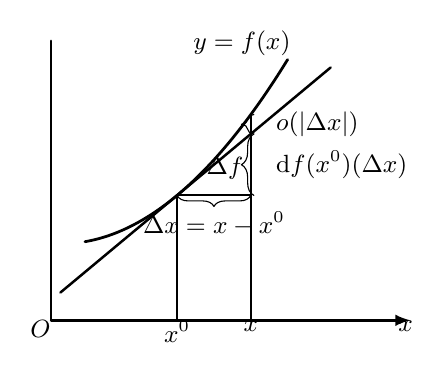
\begin{tikzpicture}[x=0.78cm, y=0.78cm, >=latex, line cap=round, line join=round]
    % ---------- 坐标架 ----------
    \draw[line width=0.9pt] (0, 0) -- (0, 4.55);
    \draw[line width=0.9pt, ->] (0, 0) -- (5.85, 0);
    \node[below left=-1pt, inner sep=1pt] at (0, 0) {\small $O$};
    \node[below left=-1pt, inner sep=1pt] at (5.90, 0) {\small $x$};
    % ---------- 曲线 y = f(x) ----------
    \draw[line width=1.0pt, domain=0.55:3.85, samples=80]
      plot (\x, {1.28 + 0.1727*(\x-0.55) + 0.22*(\x-0.55)*(\x-0.55)});
    \node[anchor=south east, inner sep=1pt] at (3.95, 4.26) {\small $y = f(x)$};
    % ---------- 切线（过 P_0 = (x^0, f(x^0))） ----------
    \draw[line width=0.9pt] (0.15, 0.452) -- (4.55, 4.116);
    % ---------- 竖直/水平辅助线 ----------
    \draw[line width=0.8pt] (2.05, 0) -- (2.05, 2.034);
    \draw[line width=0.8pt] (3.25, 0) -- (3.25, 3.350);
    \draw[line width=0.8pt] (2.05, 2.034) -- (3.25, 2.034);
    \node[below=-1pt, inner sep=1pt] at (2.05, 0) {\small $x^{0}$};
    \node[below=-1pt, inner sep=1pt] at (3.25, 0) {\small $x$};
    % ---------- 大括号与注记 ----------
    \draw[decorate, decoration={brace, amplitude=4pt, mirror}] (2.05, 2.034) -- (3.25, 2.034);
    \node[below=4pt, inner sep=1pt] at (2.65, 2.00) {\small $\Delta x = x - x^{0}$};
    \draw[decorate, decoration={brace, amplitude=4.5pt}] (3.30, 2.034) -- (3.30, 3.033);
    \draw[decorate, decoration={brace, amplitude=4.5pt}] (3.30, 3.033) -- (3.30, 3.350);
    \node[right=6pt, inner sep=1pt] at (3.34, 2.53) {\small $\mathrm{d}f(x^{0})(\Delta x)$};
    \node[right=6pt, inner sep=1pt] at (3.34, 3.19) {\small $o(|\Delta x|)$};
    \node[anchor=east, inner sep=1pt] at (3.18, 2.47) {\small $\Delta f$};
  \end{tikzpicture}
  \caption{}\label{fig:8.2.1}
\end{figure}

\begin{proof}
($\Rightarrow$) 因为 $f$ 在 $x^{0}$ 点可微, 即
\[
  f(x) - f(x^{0}) = A(x - x^{0}) + o(|x - x^{0}|) = A(x - x^{0}) + o(x - x^{0}),
\]
则
\begin{align*}
  \lim_{x \to x^{0}}\frac{f(x) - f(x^{0})}{x - x^{0}}
  &= \lim_{x \to x^{0}}\Big[A + \frac{o(|x - x^{0}|)}{x - x^{0}}\Big] \\
  &= A + 0 = A,
\end{align*}
从而 $f$ 在 $x^{0}$ 点处可导, 且 $f'(x^{0}) = A$.

($\Leftarrow$) 因为 $f$ 在 $x^{0}$ 点可导, 所以
\begin{align*}
  \lim_{x \to x^{0}}\frac{f(x) - f(x^{0}) - f'(x^{0})(x - x^{0})}{x - x^{0}}
  &= \lim_{x \to x^{0}}\Big[\frac{f(x) - f(x^{0})}{x - x^{0}} - f'(x^{0})\Big] \\
  &= f'(x^{0}) - f'(x^{0}) = 0.
\end{align*}
由此得到
\[
  f(x) - f(x^{0}) - f'(x^{0})(x - x^{0}) = o(|x - x^{0}|),
\]
\[
  f(x) - f(x^{0}) = f'(x^{0})(x - x^{0}) + o(|x - x^{0}|).
\]
这就证明了 $f$ 在点 $x^{0}$ 处是可微的.
\end{proof}

\cref{thm:8.2.2}表明, 当 $n = 1$ 时, $f$ 在 $x^{0}$ 可微与可导是彼此等价的. 是否可以指望当 $n \geqslant 2$ 时, $f$ 在 $x^{0}$ 点可微与 $f$ 在 $x^{0}$ 点有偏导数是彼此等价的呢? 下面的定理给出了明确的回答.

\begin{theorem}[可微的必要条件]\label{thm:8.2.3}
$n$ 元函数 $f$ 在 $\boldsymbol{x}^{0}$ 点处可微, 则 $f$ 在 $\boldsymbol{x}^{0}$ 点处有一阶偏导数 $f_{x_{i}}'(\boldsymbol{x}^{0})$, $i = 1, 2, \cdots, n$, 且 $\boldsymbol{A} = \boldsymbol{J}\boldsymbol{f}(\boldsymbol{x}^{0}) = (f_{x_{1}}'(\boldsymbol{x}^{0}), f_{x_{2}}'(\boldsymbol{x}^{0}), \cdots, f_{x_{n}}'(\boldsymbol{x}^{0}))$. 但反之不真.
\end{theorem}

\begin{proof}
设 $n$ 元函数 $f$ 在 $\boldsymbol{x}^{0}$ 点处可微, 令
\[
  x_{j} - x_{j}^{0} = 0, \quad j = 1, 2, \cdots, i - 1, i + 1, \cdots, n,
\]
可以得到
\begin{align*}
  &f(x_{1}^{0}, x_{2}^{0}, \cdots, x_{i-1}^{0}, x_{i}, x_{i+1}^{0}, \cdots, x_{n}^{0}) - f(x_{1}^{0}, x_{2}^{0}, \cdots, x_{i-1}^{0}, x_{i}^{0}, x_{i+1}^{0}, \cdots, x_{n}^{0}) \\
  &= a_{i}(x_{i} - x_{i}^{0}) + o(|x_{i} - x_{i}^{0}|) = a_{i}(x_{i} - x_{i}^{0}) + o(x_{i} - x_{i}^{0}).
\end{align*}
于是,
\begin{align*}
  f_{x_{i}}'(\boldsymbol{x}^{0})
  &= \lim_{x_{i} \to x_{i}^{0}}\frac{f(x_{1}^{0}, x_{2}^{0}, \cdots, x_{i-1}^{0}, x_{i}, x_{i+1}^{0}, \cdots, x_{n}^{0}) - f(x_{1}^{0}, x_{2}^{0}, \cdots, x_{i-1}^{0}, x_{i}^{0}, x_{i+1}^{0}, \cdots, x_{n}^{0})}{x_{i} - x_{i}^{0}} \\
  &= \lim_{x_{i} \to x_{i}^{0}}\frac{a_{i}(x_{i} - x_{i}^{0}) + o(x_{i} - x_{i}^{0})}{x_{i} - x_{i}^{0}} \\
  &= \lim_{x_{i} \to x_{i}^{0}}\Big[a_{i} + \frac{o(x_{i} - x_{i}^{0})}{x_{i} - x_{i}^{0}}\Big] = a_{i} + 0 = a_{i}, \quad i = 1, 2, \cdots, n.
\end{align*}
但反之不真. 例如
\[
  f(x, y) = \begin{cases}
    \dfrac{xy}{x^{2} + y^{2}}, & (x, y) \neq (0, 0), \\[2.5mm]
    0, & (x, y) = (0, 0),
  \end{cases}
\]
易见
\[
  f_{x}'(0, 0) = \lim_{x \to 0}\frac{f(x, 0) - f(0, 0)}{x - 0} = \lim_{x \to 0}0 = 0,
\]
\[
  f_{y}'(0, 0) = \lim_{y \to 0}\frac{f(0, y) - f(0, 0)}{y - 0} = \lim_{y \to 0}0 = 0,
\]
所以
\[
  \boldsymbol{J}f(0, 0) = (f_{x}'(0, 0), f_{y}'(0, 0)) = (0, 0).
\]
\[
  f(x, y) - f(0, 0) = \frac{xy}{x^{2} + y^{2}} - 0 = (0, 0)\binom{x - 0}{y - 0} + \frac{xy}{x^{2} + y^{2}},
\]
现证 $\dfrac{xy}{x^{2} + y^{2}} \neq o(\sqrt{x^{2} + y^{2}})$.

(反证) 假设 $\dfrac{xy}{x^{2} + y^{2}} = o(\sqrt{x^{2} + y^{2}})$, 则
\[
  \lim_{(x, y) \to (0, 0)}\frac{xy}{x^{2} + y^{2}} = \lim_{(x, y) \to (0, 0)}\frac{\dfrac{xy}{x^{2} + y^{2}}}{\sqrt{x^{2} + y^{2}}}\sqrt{x^{2} + y^{2}} = 0 \times 0 = 0.
\]
这与\cref{ex:7.5.5}中二重极限不存在相矛盾. 由上述得到 $f$ 在 $(0, 0)$ 处不可微.

或者从 $\lim_{\substack{x \to 0 \\ y \to 0}}\dfrac{xy}{x^{2} + y^{2}}$ 不存在及\cref{thm:8.2.1}推得 $f$ 在 $(0, 0)$ 处不可微.
\end{proof}

\begin{remark}\label{rem:8.2.1}
因为
\[
  \mathrm{d}f(\boldsymbol{x}^{0})(\Delta\boldsymbol{x}) = \sum_{i=1}^{n}\frac{\partial f}{\partial x_{i}}(\boldsymbol{x}^{0})\Delta x_{i} = \Big(\sum_{i=1}^{n}\frac{\partial f}{\partial x_{i}}(\boldsymbol{x}^{0})\mathrm{d}x_{i}\Big)(\Delta\boldsymbol{x}),
\]
所以
\[
  \mathrm{d}f(\boldsymbol{x}^{0}) = \sum_{i=1}^{n}\frac{\partial f}{\partial x_{i}}(\boldsymbol{x}^{0})\mathrm{d}x_{i},
\]
并称
\[
  \mathrm{d}f = \sum_{i=1}^{n}\frac{\partial f}{\partial x_{i}}\mathrm{d}x_{i}
\]
为 $f$ 的 (全) 微分.
\end{remark}

\begin{theorem}[可微的充分条件]\label{thm:8.2.4}
设 $U \subset \mathbb{R}^{n}$ 为开集, $f: U \to \mathbb{R}^{1}$ 为 $n$ 元函数, 如果 $Jf = (f_{x_{1}}', f_{x_{2}}', \cdots, f_{x_{n}}')$ 在 $\boldsymbol{x}^{0}$ 连续 ($\Leftrightarrow f_{x_{i}}'$ 在 $\boldsymbol{x}^{0}$ 连续, $i = 1, 2, \cdots, n$), 则 $f$ 在 $\boldsymbol{x}^{0}$ 可微. 但反之不真.
\end{theorem}

\begin{proof}
\begin{align*}
  &f(\boldsymbol{x}) - f(\boldsymbol{x}^{0}) \\
  ={} &\sum_{i=1}^{n}\big[f(x_{1}^{0}, x_{2}^{0}, \cdots, x_{i-1}^{0}, x_{i}, x_{i+1}, \cdots, x_{n}) \\
  &\qquad - f(x_{1}^{0}, x_{2}^{0}, \cdots, x_{i-1}^{0}, x_{i}^{0}, x_{i+1}, \cdots, x_{n})\big] \\
  \reasonb{Lagrange 中值定理} {\exists\xi_{i}\ \text{在}\ x_{i}^{0}\ \text{与}\ x_{i}\ \text{之间}}
  ={} &\sum_{i=1}^{n}f_{x_{i}}'(x_{1}^{0}, x_{2}^{0}, \cdots, x_{i-1}^{0}, \xi_{i}, x_{i+1}, \cdots, x_{n})(x_{i} - x_{i}^{0}) \\
  ={} &\sum_{i=1}^{n}f_{x_{i}}'(\boldsymbol{x}^{0})(x_{i} - x_{i}^{0}) + \sum_{i=1}^{n}\alpha_{i}(x_{i} - x_{i}^{0}),
\end{align*}
其中
\begin{align*}
  \alpha_{i} &= f_{x_{i}}'(x_{1}^{0}, x_{2}^{0}, \cdots, x_{i-1}^{0}, \xi_{i}, x_{i+1}, \cdots, x_{n}) - f_{x_{i}}'(x_{1}^{0}, x_{2}^{0}, \cdots, x_{i-1}^{0}, x_{i}^{0}, x_{i+1}^{0}, \cdots, x_{n}^{0}) \\
  &\xrightarrow{Jf\ \text{在}\ \boldsymbol{x}^{0}\ \text{处连续}}\ 0 \quad (\|\boldsymbol{x} - \boldsymbol{x}^{0}\| \to 0). \\
  0 &\leqslant \frac{\big|\sum_{i=1}^{n}\alpha_{i}(x_{i} - x_{i}^{0})\big|}{\|\boldsymbol{x} - \boldsymbol{x}^{0}\|} = \Big|\sum_{i=1}^{n}\alpha_{i}\frac{x_{i} - x_{i}^{0}}{\sqrt{\sum_{j=1}^{n}(x_{j} - x_{j}^{0})^{2}}}\Big| \leqslant \sum_{i=1}^{n}|\alpha_{i}| \to 0 \quad (\|\boldsymbol{x} - \boldsymbol{x}^{0}\| \to 0),
\end{align*}
所以
\[
  \lim_{\boldsymbol{x} \to \boldsymbol{x}^{0}}\frac{\sum_{i=1}^{n}\alpha_{i}(x_{i} - x_{i}^{0})}{\|\boldsymbol{x} - \boldsymbol{x}^{0}\|} = 0,
\]
\[
  f(\boldsymbol{x}) - f(\boldsymbol{x}^{0}) = \sum_{i=1}^{n}f_{x_{i}}'(\boldsymbol{x}^{0})(x_{i} - x_{i}^{0}) + o(\|\boldsymbol{x} - \boldsymbol{x}^{0}\|),
\]
这就证明了 $f$ 在 $\boldsymbol{x}^{0}$ 可微.

但反之不真. 例如: $f: \mathbb{R}^{1} \to \mathbb{R}^{1}$, $x \mapsto f(x)$,
\[
  f(x) = \begin{cases}
    x^{2}\sin\dfrac{1}{x}, & x \neq 0, \\[2.5mm]
    0, & x = 0,
  \end{cases}
\]
\[
  f'(x) = \begin{cases}
    2x\sin\dfrac{1}{x} - \cos\dfrac{1}{x}, & x \neq 0, \\[2.5mm]
    0, & x = 0.
  \end{cases}
\]
根据\cref{thm:8.2.2}, $f$ 在 $0$ 可导 $\Leftrightarrow f$ 在 $0$ 可微. 然而 $f'$ 在 $0$ 不连续.
\end{proof}

可微概念可从 $n$ 元函数继续推广到 Euclid 空间之间的映射.

\begin{definition}\label{def:8.2.2}
设 $U \subset \mathbb{R}^{n}$ 为开集, $f: U \to \mathbb{R}^{m}$ 为映射,
\begin{align*}
  \boldsymbol{x}^{0} &= \begin{pmatrix} x_{1}^{0} \\ \vdots \\ x_{n}^{0} \end{pmatrix} \in U, \quad
  \boldsymbol{x} = \begin{pmatrix} x_{1} \\ \vdots \\ x_{n} \end{pmatrix} \in U, \quad
  \Delta\boldsymbol{x} = \begin{pmatrix} \Delta x_{1} \\ \vdots \\ \Delta x_{n} \end{pmatrix}
  = \begin{pmatrix} x_{1} - x_{1}^{0} \\ \vdots \\ x_{n} - x_{n}^{0} \end{pmatrix} = \boldsymbol{x} - \boldsymbol{x}^{0} \in \mathbb{R}^{n}, \\
  \boldsymbol{f} &= \begin{pmatrix} f_{1} \\ \vdots \\ f_{m} \end{pmatrix}, \quad
  \boldsymbol{A} = \begin{pmatrix} a_{11} & \cdots & a_{1n} \\ \vdots & \ddots & \vdots \\ a_{m1} & \cdots & a_{mn} \end{pmatrix}
\end{align*}
其中 $\boldsymbol{A}$ 为 $m \times n$ 的实矩阵. 如果
\[
  f(\boldsymbol{x}^{0} + \Delta\boldsymbol{x}) - f(\boldsymbol{x}^{0}) = \boldsymbol{A}\Delta\boldsymbol{x} + \boldsymbol{R}(\Delta\boldsymbol{x}), \quad \boldsymbol{R}(\Delta\boldsymbol{x}) = o(\|\Delta\boldsymbol{x}\|), \quad \|\Delta\boldsymbol{x}\| \to 0,
\]
即
\[
  f(\boldsymbol{x}) - f(\boldsymbol{x}^{0}) = \boldsymbol{A}(\boldsymbol{x} - \boldsymbol{x}^{0}) + \boldsymbol{R}(\boldsymbol{x} - \boldsymbol{x}^{0}), \quad \boldsymbol{R}(\boldsymbol{x} - \boldsymbol{x}^{0}) = o(\|\boldsymbol{x} - \boldsymbol{x}^{0}\|), \quad \|\boldsymbol{x} - \boldsymbol{x}^{0}\| \to 0,
\]
则称映射 $f$ 在 $\boldsymbol{x}^{0}$ \textbf{可微}. 记
\[
  \mathrm{d}f(\boldsymbol{x}^{0}): \mathbb{R}^{n} \to \mathbb{R}^{m},
\]
\[
  \mathrm{d}f(\boldsymbol{x}^{0})(\Delta\boldsymbol{x}) = \boldsymbol{A}\Delta\boldsymbol{x},
\]
即
\[
  \mathrm{d}f(\boldsymbol{x}^{0})(\boldsymbol{x} - \boldsymbol{x}^{0}) = \boldsymbol{A}(\boldsymbol{x} - \boldsymbol{x}^{0}).
\]
显然, $\mathrm{d}f(\boldsymbol{x}^{0})$ 为线性映射, 称 $\mathrm{d}f(\boldsymbol{x}^{0})$ 为 $f$ 在点 $\boldsymbol{x}^{0} \in U$ 处的\textbf{微分}.
\end{definition}

考虑分量形式为
\[
  \begin{pmatrix} f_{1}(\boldsymbol{x}^{0} + \Delta\boldsymbol{x}) - f_{1}(\boldsymbol{x}^{0}) \\ \vdots \\ f_{m}(\boldsymbol{x}^{0} + \Delta\boldsymbol{x}) - f_{m}(\boldsymbol{x}^{0}) \end{pmatrix}
  = \begin{pmatrix} a_{11} & \cdots & a_{1n} \\ \vdots & & \vdots \\ a_{m1} & \cdots & a_{mn} \end{pmatrix}
    \begin{pmatrix} \Delta x_{1} \\ \vdots \\ \Delta x_{n} \end{pmatrix}
  + \begin{pmatrix} R_{1}(\Delta\boldsymbol{x}) \\ \vdots \\ R_{m}(\Delta\boldsymbol{x}) \end{pmatrix}
\]
\[
  \Leftrightarrow f_{i}(\boldsymbol{x}^{0} + \Delta\boldsymbol{x}) - f_{i}(\boldsymbol{x}^{0}) = (a_{i1}, a_{i2}, \cdots, a_{in})\begin{pmatrix} \Delta x_{1} \\ \vdots \\ \Delta x_{n} \end{pmatrix} + R_{i}(\Delta\boldsymbol{x}),
\]
\[
  R_{i}(\Delta\boldsymbol{x}) = o(\|\Delta\boldsymbol{x}\|), \quad \|\Delta\boldsymbol{x}\| \to 0, \quad i = 1, 2, \cdots, m.
\]
$\Leftrightarrow f_{i}$ 在 $\boldsymbol{x}^{0}$ 是可微的, $i = 1, 2, \cdots, m$.

读者可用另一形式 (即 $\boldsymbol{x}$, $\boldsymbol{x} - \boldsymbol{x}^{0}$) 表达上述式子.

由上述讨论立即有下面定理.

\begin{theorem}\label{thm:8.2.5}
设 $U \subset \mathbb{R}^{n}$ 为开集, 映射 $f: U \to \mathbb{R}^{m}$ 在 $\boldsymbol{x}^{0} \in U$ 可微 $\Leftrightarrow n$ 元函数 $f_{i}\ (i = 1, 2, \cdots, m)$ 在 $\boldsymbol{x}^{0}$ 点可微.
\end{theorem}

类似 $n$ 元函数的\cref{thm:8.2.1}, \cref{thm:8.2.3}, \cref{thm:8.2.4}, 关于映射也有以下相应的定理.

\setcounter{theorem}{1}
\begin{theoremp}\label{thm:8.2.1p}
设 $U \subset \mathbb{R}^{n}$ 为开集, 映射 $f: U \to \mathbb{R}^{m}$ 在 $\boldsymbol{x}^{0}$ 处可微, 必有 $f$ 在 $\boldsymbol{x}^{0}$ 处连续. 但反之不真.
\end{theoremp}

\begin{proof}
类似\cref{thm:8.2.1}的证明.
\end{proof}

\setcounter{theorem}{3}
\begin{theoremp}[可微的必要条件]\label{thm:8.2.3p}
设 $U \subset \mathbb{R}^{n}$ 为开集, $f: U \to \mathbb{R}^{n}$ 为映射, 且 $f$ 在 $\boldsymbol{x}^{0}$ 点处可微, 则 $\dfrac{\partial f_{i}}{\partial x_{j}}(\boldsymbol{x}^{0})$ 存在有限, 且
\[
  \boldsymbol{A} = \Big(\frac{\partial f_{i}}{\partial x_{j}}\Big)\Big|_{\boldsymbol{x}^{0}} = \begin{pmatrix}
    \dfrac{\partial f_{1}}{\partial x_{1}} & \cdots & \dfrac{\partial f_{1}}{\partial x_{n}} \\[2mm]
    \vdots & & \vdots \\[1mm]
    \dfrac{\partial f_{m}}{\partial x_{1}} & \cdots & \dfrac{\partial f_{m}}{\partial x_{n}}
  \end{pmatrix}_{\boldsymbol{x}^{0}} = \boldsymbol{J}\boldsymbol{f}(\boldsymbol{x}^{0}) = \mathrm{grad}\,f\Big|_{\boldsymbol{x}^{0}},
\]
并称 $\mathrm{grad}\,f\big|_{\boldsymbol{x}^{0}} = Jf(\boldsymbol{x}^{0})$ 为 $f$ 在 $\boldsymbol{x}^{0}$ 处的 Jacobi 矩阵, 或 $f$ 在 $\boldsymbol{x}^{0}$ 的``导数'', 或 $f$ 的\textbf{梯度} (gradient). 但反之不真.
\end{theoremp}

\begin{proof}
$f$ 在 $\boldsymbol{x}^{0}$ 处可微 $\Leftrightarrow f_{i}$ 在 $\boldsymbol{x}^{0}$ 处可微, $i = 1, 2, \cdots, m$, 由\cref{thm:8.2.3}可知, $\dfrac{\partial f_{i}}{\partial x_{j}}(\boldsymbol{x}^{0})$ 存在有限, $i = 1, 2, \cdots, m$; $j = 1, 2, \cdots, n$.

但反之不真. 反例见\cref{thm:8.2.3}中的反例.
\end{proof}

如果 $f$ 在任何 $\boldsymbol{x} \in U \subset \mathbb{R}^{n}$ 有偏导数, 则
\[
  Jf: U \to \mathbb{R}^{mn},
\]
\[
  \boldsymbol{x} \mapsto \boldsymbol{J}\boldsymbol{f}(\boldsymbol{x}) = \begin{pmatrix}
    \dfrac{\partial f_{1}}{\partial x_{1}} & \cdots & \dfrac{\partial f_{1}}{\partial x_{n}} \\[2mm]
    \vdots & & \vdots \\[1mm]
    \dfrac{\partial f_{m}}{\partial x_{1}} & \cdots & \dfrac{\partial f_{m}}{\partial x_{n}}
  \end{pmatrix}_{\boldsymbol{x}}
\]
为一映射. 于是
\[
  \mathrm{d}f(\boldsymbol{x}^{0})(\Delta\boldsymbol{x}) = Jf(\boldsymbol{x}^{0})\Delta\boldsymbol{x}.
\]
令
\[
  \mathrm{d}x_{i}(\Delta x_{j}) = \delta_{ij} = \begin{cases}
    1, & i \neq j, \\
    0, & i = j,
  \end{cases}
\]
则
\[
  \mathrm{d}f_{i}\Big|_{\boldsymbol{x}^{0}} = \sum_{j=1}^{n}\frac{\partial f_{i}}{\partial x_{j}}(\boldsymbol{x}^{0})\mathrm{d}x_{j},
\]
\[
  \mathrm{d}\boldsymbol{f}\Big|_{\boldsymbol{x}^{0}} = \begin{pmatrix} \mathrm{d}f_{1} \\ \vdots \\ \mathrm{d}f_{m} \end{pmatrix}\Big|_{\boldsymbol{x}^{0}} = \begin{pmatrix}
    \displaystyle\sum_{j=1}^{n}\frac{\partial f_{1}}{\partial x_{j}}(\boldsymbol{x}^{0})\mathrm{d}x_{j} \\ \vdots \\
    \displaystyle\sum_{j=1}^{n}\frac{\partial f_{m}}{\partial x_{j}}(\boldsymbol{x}^{0})\mathrm{d}x_{j}
  \end{pmatrix}
\]
\[
  = \begin{pmatrix}
    \displaystyle\frac{\partial f_{1}}{\partial x_{1}} & \cdots & \displaystyle\frac{\partial f_{1}}{\partial x_{n}} \\[3mm]
    \vdots & & \vdots \\[2mm]
    \displaystyle\frac{\partial f_{m}}{\partial x_{1}} & \cdots & \displaystyle\frac{\partial f_{m}}{\partial x_{n}}
  \end{pmatrix}_{\boldsymbol{x}^{0}} \begin{pmatrix} \mathrm{d}x_{1} \\ \vdots \\ \mathrm{d}x_{n} \end{pmatrix} = \boldsymbol{J}\boldsymbol{f}(\boldsymbol{x}^{0})\mathrm{d}\boldsymbol{x},
\]
并称它为映射 $f$ 的 (全) 微分.

\setcounter{theorem}{4}
\begin{theoremp}[可微的充分条件]\label{thm:8.2.4p}
设 $U \subset \mathbb{R}^{n}$ 为开集, $f: U \to \mathbb{R}^{m}$ 为映射, 如果 $f$ 的 Jacobi 矩阵 $Jf = \Big(\dfrac{\partial f_{i}}{\partial x_{j}}\Big)$ 在 $\boldsymbol{x}^{0}$ 连续, 则 $f$ 在 $\boldsymbol{x}^{0}$ 可微. 但反之不真.
\end{theoremp}

\begin{proof}
\begin{align*}
  Jf = \Big(\frac{\partial f_{i}}{\partial x_{j}}\Big)\ \text{在}\ \boldsymbol{x}^{0}\ \text{连续}
  &\Leftrightarrow Jf_{i}\ \text{在}\ \boldsymbol{x}^{0}\ \text{连续},\ i = 1, 2, \cdots, m \\
  &\overset{\text{定理}\ 8.2.4}{\Longleftrightarrow} f_{i}\ \text{在}\ \boldsymbol{x}^{0}\ \text{可微},\ i = 1, 2, \cdots, m \\
  &\overset{\text{定理}\ 8.2.5}{\Longleftrightarrow} f\ \text{在}\ \boldsymbol{x}^{0}\ \text{可微}. \qedhere
\end{align*}
\end{proof}

\setcounter{theorem}{5}
\begin{remark}\label{rem:8.2.2}
从\cref{thm:8.2.3p}与\cref{thm:8.2.4p}可知, $f$ 的一阶偏导数 $\dfrac{\partial f_{i}}{\partial x_{j}}$ 在 $\boldsymbol{x}^{0}$ 连续 $\Rightarrow f$ 在 $\boldsymbol{x}^{0}$ 可微 $\Rightarrow f$ 在 $\boldsymbol{x}^{0}$ 有一阶偏导数 $\dfrac{\partial f_{i}}{\partial x_{j}}$, $i = 1, 2, \cdots, m$; $j = 1, 2, \cdots, n$. 因此, 可微是介于 $f$ 的一阶偏导数在 $\boldsymbol{x}^{0}$ 连续与 $f$ 在 $\boldsymbol{x}^{0}$ 有一阶偏导数之间的一个概念.
\end{remark}

\begin{definition}\label{def:8.2.3}
设 $U \subset \mathbb{R}^{n}$ 为开集, $f: U \to \mathbb{R}^{m}$ 为 $C^{k}$ 映射:

$k = 0$, $f$ 为连续映射;

$0 < k < +\infty$, $f_{i}$ 有直到 $k$ 阶连续偏导数, $i = 1, 2, \cdots, m$;

$k = +\infty$, $f_{i}$ 具有各阶连续偏导数, $i = 1, 2, \cdots, m$;

$k = \omega$, $f_{i}$ 实解析, 即在 $U$ 中任一点 $\boldsymbol{x}^{0} = (x_{1}^{0}, x_{2}^{0}, \cdots, x_{n}^{0})$ 的邻近可展开为收敛的 ($n$ 元) 幂级数, $i = 1, 2, \cdots, m$.

记 $C^{k}(U, \mathbb{R}^{m})$ 为从 $U$ 到 $\mathbb{R}^{m}$ 的 $C^{k}$ 映射的全体.
\end{definition}

将\cref{thm:8.1.3}推广为映射的复合求导链规则有下面的定理.

\begin{theorem}[映射的复合求导的链规则]\label{thm:8.2.6}
设 $U \subset \mathbb{R}^{l}$ 与 $V \subset \mathbb{R}^{n}$ 都为开集,
\[
  \boldsymbol{g}: U \to V \quad \text{与} \quad f: V \to \mathbb{R}^{m}
\]
都为映射, $\boldsymbol{g}$ 在 $\boldsymbol{u}^{0} \in U$ 可微, $f$ 在 $\boldsymbol{x}^{0} = \boldsymbol{g}(\boldsymbol{u}^{0})$ 可微, 则复合映射 $f \circ \boldsymbol{g}$ 在 $\boldsymbol{u}^{0}$ 也可微, 且
\[
  \boldsymbol{J}(f \circ \boldsymbol{g})'(\boldsymbol{u}^{0}) = \boldsymbol{J}f(\boldsymbol{x}^{0})\boldsymbol{J}\boldsymbol{g}(\boldsymbol{u}^{0}).
\]
\end{theorem}

\begin{proof}
$\boldsymbol{g}$ 在 $\boldsymbol{u}^{0}$ 可微, 即
\[
  \boldsymbol{g}(\boldsymbol{u}) - \boldsymbol{g}(\boldsymbol{u}^{0}) = \boldsymbol{J}\boldsymbol{g}(\boldsymbol{u}^{0})(\boldsymbol{u} - \boldsymbol{u}^{0}) + \boldsymbol{R}_{g}(\boldsymbol{u} - \boldsymbol{u}^{0}),
\]
\[
  \boldsymbol{R}_{g}(\boldsymbol{u} - \boldsymbol{u}^{0}) = o(\boldsymbol{u} - \boldsymbol{u}^{0}), \quad \boldsymbol{u} \to \boldsymbol{u}^{0}.
\]
又 $f$ 在 $\boldsymbol{x}^{0} = \boldsymbol{g}(\boldsymbol{u}^{0})$ 可微, 故
\[
  f(\boldsymbol{x}) - f(\boldsymbol{x}^{0}) = Jf(\boldsymbol{x}^{0})(\boldsymbol{x} - \boldsymbol{x}^{0}) + R_{f}(\boldsymbol{x} - \boldsymbol{x}^{0}),
\]
\[
  \boldsymbol{R}_{f}(\boldsymbol{x} - \boldsymbol{x}^{0}) = o(\boldsymbol{x} - \boldsymbol{x}^{0}), \quad \boldsymbol{x} \to \boldsymbol{x}^{0}.
\]
令 $\boldsymbol{x} = \boldsymbol{g}(\boldsymbol{u})$, $\boldsymbol{x}^{0} = \boldsymbol{g}(\boldsymbol{u}^{0})$ 代入上式得到
\begin{align*}
  f \circ \boldsymbol{g}(\boldsymbol{u}) - f \circ \boldsymbol{g}(\boldsymbol{u}^{0})
  &= \boldsymbol{J}f(\boldsymbol{x}^{0})(\boldsymbol{g}(\boldsymbol{u}) - \boldsymbol{g}(\boldsymbol{u}^{0})) + \boldsymbol{R}_{f}(\boldsymbol{g}(\boldsymbol{u}) - \boldsymbol{g}(\boldsymbol{u}^{0})) \\
  &= \boldsymbol{J}f(\boldsymbol{x}^{0})\big[\boldsymbol{J}\boldsymbol{g}(\boldsymbol{u}^{0})(\boldsymbol{u} - \boldsymbol{u}^{0}) + \boldsymbol{R}_{g}(\boldsymbol{u} - \boldsymbol{u}^{0})\big] + \boldsymbol{R}_{f}(\boldsymbol{g}(\boldsymbol{u}) - \boldsymbol{g}(\boldsymbol{u}^{0})) \\
  &= \boldsymbol{J}f(\boldsymbol{x}^{0})\boldsymbol{J}\boldsymbol{g}(\boldsymbol{u}^{0})(\boldsymbol{u} - \boldsymbol{u}^{0}) + \boldsymbol{R}_{f \circ g}(\boldsymbol{u} - \boldsymbol{u}^{0}),
\end{align*}
其中
\[
  \|\boldsymbol{J}f(\boldsymbol{x}^{0})\boldsymbol{R}_{g}(\boldsymbol{u} - \boldsymbol{u}^{0})\| \overset{\text{8.2 练习题 26}}{\leqslant} \|\boldsymbol{J}f(\boldsymbol{x}^{0})\|\|\boldsymbol{R}_{g}(\boldsymbol{u} - \boldsymbol{u}^{0})\| = o(\boldsymbol{u} - \boldsymbol{u}^{0}),
\]
\[
  \text{矩阵}\ \boldsymbol{A}\ \text{的模}\quad \|\boldsymbol{A}\| = \sqrt{\sum_{i=1}^{m}\sum_{j=1}^{n}a_{ij}^{2}}.
\]
\begin{align*}
  0 \leqslant {}& \frac{\|\boldsymbol{R}_{f}(\boldsymbol{g}(\boldsymbol{u}) - \boldsymbol{g}(\boldsymbol{u}^{0}))\|}{\|\boldsymbol{u} - \boldsymbol{u}^{0}\|} \\
  = {}& \frac{\|\boldsymbol{R}_{f}(\boldsymbol{g}(\boldsymbol{u}) - \boldsymbol{g}(\boldsymbol{u}^{0}))\|}{\|\boldsymbol{g}(\boldsymbol{u}) - \boldsymbol{g}(\boldsymbol{u}^{0})\|} \cdot \frac{\|\boldsymbol{g}(\boldsymbol{u}) - \boldsymbol{g}(\boldsymbol{u}^{0})\|}{\|\boldsymbol{u} - \boldsymbol{u}^{0}\|} \\
  \leqslant {}& \frac{\|\boldsymbol{R}_{f}(\boldsymbol{g}(\boldsymbol{u}) - \boldsymbol{g}(\boldsymbol{u}^{0}))\|}{\|\boldsymbol{g}(\boldsymbol{u}) - \boldsymbol{g}(\boldsymbol{u}^{0})\|}\Big[\|\boldsymbol{J}\boldsymbol{g}(\boldsymbol{u}^{0})\| + \frac{\|\boldsymbol{R}_{g}(\boldsymbol{u} - \boldsymbol{u}^{0})\|}{\boldsymbol{u} - \boldsymbol{u}^{0}}\Big] \\
  \to {}& 0 \quad (\boldsymbol{u} \to \boldsymbol{u}^{0},\ \text{由}\ \boldsymbol{g}\ \text{连续知},\ \boldsymbol{g}(\boldsymbol{u}) \to \boldsymbol{g}(\boldsymbol{u}^{0}));
\end{align*}
注意, 当 $\boldsymbol{g}(\boldsymbol{u}) = \boldsymbol{g}(\boldsymbol{u}^{0})$ 时, 上式也有
\[
  \frac{\|\boldsymbol{R}_{f}(\boldsymbol{g}(\boldsymbol{u}) - \boldsymbol{g}(\boldsymbol{u}^{0}))\|}{\|\boldsymbol{u} - \boldsymbol{u}^{0}\|} = \frac{\|\boldsymbol{R}_{f}(\boldsymbol{0})\|}{\|\boldsymbol{u} - \boldsymbol{u}^{0}\|} = 0 \to 0 \quad (\boldsymbol{u} \to \boldsymbol{u}^{0}).
\]
因此 $f \circ \boldsymbol{g}$ 在 $\boldsymbol{u}^{0}$ 可微, 且
\[
  \boldsymbol{J}(f \circ \boldsymbol{g})(\boldsymbol{u}^{0}) = \boldsymbol{J}f(\boldsymbol{x}^{0})\boldsymbol{J}\boldsymbol{g}(\boldsymbol{u}^{0}).
\]
\end{proof}

\begin{remark}\label{rem:8.2.3}
\[
  \boldsymbol{y} = f(\boldsymbol{x}), \quad \boldsymbol{x} = \boldsymbol{g}(\boldsymbol{u}),
\]
\[
  \boldsymbol{J}(f \circ \boldsymbol{g})(\boldsymbol{u}^{0}) = \boldsymbol{J}f(\boldsymbol{x}^{0})\boldsymbol{J}\boldsymbol{g}(\boldsymbol{u}^{0}),
\]
其分量形式表达为
\[
  \begin{pmatrix} y_{1} \\ \vdots \\ y_{m} \end{pmatrix} = \begin{pmatrix} f_{1}(x_{1}, \cdots, x_{n}) \\ \vdots \\ f_{m}(x_{1}, \cdots, x_{n}) \end{pmatrix}, \quad
  \begin{pmatrix} x_{1} \\ \vdots \\ x_{n} \end{pmatrix} = \begin{pmatrix} g_{1}(u_{1}, \cdots, u_{l}) \\ \vdots \\ g_{n}(u_{1}, \cdots, u_{l}) \end{pmatrix},
\]
\[
  \begin{pmatrix}
    \displaystyle\frac{\partial y_{1}}{\partial u_{1}} & \cdots & \displaystyle\frac{\partial y_{1}}{\partial u_{l}} \\[3mm]
    \vdots & & \vdots \\[2mm]
    \displaystyle\frac{\partial y_{m}}{\partial u_{1}} & \cdots & \displaystyle\frac{\partial y_{m}}{\partial u_{l}}
  \end{pmatrix} = \begin{pmatrix}
    \displaystyle\frac{\partial y_{1}}{\partial x_{1}} & \cdots & \displaystyle\frac{\partial y_{1}}{\partial x_{n}} \\[3mm]
    \vdots & & \vdots \\[2mm]
    \displaystyle\frac{\partial y_{m}}{\partial x_{1}} & \cdots & \displaystyle\frac{\partial y_{m}}{\partial x_{n}}
  \end{pmatrix}\begin{pmatrix}
    \displaystyle\frac{\partial x_{1}}{\partial u_{1}} & \cdots & \displaystyle\frac{\partial x_{1}}{\partial u_{l}} \\[3mm]
    \vdots & & \vdots \\[2mm]
    \displaystyle\frac{\partial x_{n}}{\partial u_{1}} & \cdots & \displaystyle\frac{\partial x_{n}}{\partial u_{l}}
  \end{pmatrix},
\]
即
\[
  \frac{\partial y_{i}}{\partial u_{j}} = \sum_{k=1}^{n}\frac{\partial y_{i}}{\partial x_{k}}\frac{\partial x_{k}}{\partial u_{j}}, \quad i = 1, 2, \cdots, m; \quad j = 1, 2, \cdots, l.
\]
\end{remark}

这就是多变量函数求导的链规则公式. 最后一式适合于单个分量 $y_{i}$ 的求导, 因为它不涉及到其他分量 $y_{j}$ 的求导, 所以不必大张旗鼓地应用上述矩阵公式来计算.

应该指出, 上述矩阵公式特别适用于全部分量 $y_{i}$ 的偏导数计算与整体性论证的简捷表达.

可微定义可以换成下面的等价形式, 它在使用时比较方便.

\begin{theorem}\label{thm:8.2.7}
设 $U \subset \mathbb{R}^{n}$ 为开集, 则

映射 $f: U \to \mathbb{R}^{m}$ 在点 $\boldsymbol{x}^{0}$ 处可微 $\Leftrightarrow$
\[
  f(\boldsymbol{x}^{0} + \Delta\boldsymbol{x}) - f(\boldsymbol{x}^{0}) = Jf(\boldsymbol{x}^{0})\Delta\boldsymbol{x} + B(\Delta\boldsymbol{x})\Delta\boldsymbol{x},
\]
其中 $B(\Delta\boldsymbol{x})$ 为 $m \times n$ 矩阵, 且
\[
  \lim_{\Delta\boldsymbol{x} \to \boldsymbol{0}}\boldsymbol{B}(\Delta\boldsymbol{x}) = \boldsymbol{0}.
\]
\end{theorem}

\begin{proof}
($\Leftarrow$) 显然有
\[
  0 \leqslant \frac{1}{\|\Delta\boldsymbol{x}\|}\|\boldsymbol{B}(\Delta\boldsymbol{x})\Delta\boldsymbol{x}\| = \Big\|\boldsymbol{B}(\Delta\boldsymbol{x})\frac{\Delta\boldsymbol{x}}{\|\Delta\boldsymbol{x}\|}\Big\|
\]
\[
  \overset{\text{8.2 练习题 26}}{\leqslant} \|\boldsymbol{B}(\Delta\boldsymbol{x})\|\Big\|\frac{\Delta\boldsymbol{x}}{\|\Delta\boldsymbol{x}\|}\Big\| = \|\boldsymbol{B}(\Delta\boldsymbol{x})\| \to 0 \quad (\|\Delta\boldsymbol{x}\| \to 0).
\]
因此,
\[
  \boldsymbol{B}(\Delta\boldsymbol{x})\Delta\boldsymbol{x} = o(\|\Delta\boldsymbol{x}\|).
\]
根据\cref{def:8.2.2}, $f$ 在点 $\boldsymbol{x}^{0}$ 处可微.

($\Rightarrow$) 设 $f$ 在点 $\boldsymbol{x}^{0}$ 处可微, 则
\[
  \boldsymbol{R}_{f}(\Delta\boldsymbol{x}) = \boldsymbol{f}(\boldsymbol{x}^{0} + \Delta\boldsymbol{x}) - \boldsymbol{f}(\boldsymbol{x}^{0}) - \boldsymbol{J}\boldsymbol{f}(\boldsymbol{x}^{0})\Delta\boldsymbol{x},
\]
\[
  \boldsymbol{R}_{f}(\Delta\boldsymbol{x}) = o(\|\Delta\boldsymbol{x}\|) \quad (\|\Delta\boldsymbol{x}\| \to 0).
\]
令
\[
  \boldsymbol{B}(\Delta\boldsymbol{x}) = \begin{cases}
    \dfrac{\boldsymbol{R}_{f}(\Delta\boldsymbol{x})}{\|\Delta\boldsymbol{x}\|}\dfrac{\Delta\boldsymbol{x}}{\|\Delta\boldsymbol{x}\|}, & \Delta\boldsymbol{x} \neq \boldsymbol{0}, \\[3mm]
    \boldsymbol{0}, & \Delta\boldsymbol{x} = \boldsymbol{0}.
  \end{cases}
\]
由于
\[
  0 \leqslant \|\boldsymbol{B}(\Delta\boldsymbol{x})\| = \Big\|\frac{\boldsymbol{R}_{f}(\Delta\boldsymbol{x})}{\|\Delta\boldsymbol{x}\|}\frac{\Delta\boldsymbol{x}}{\|\Delta\boldsymbol{x}\|}\Big\| = \Big\|\frac{\boldsymbol{R}_{f}(\Delta\boldsymbol{x})}{\|\Delta\boldsymbol{x}\|}\Big\| \to 0 \quad (\|\Delta\boldsymbol{x}\| \to 0),
\]
就有
\[
  \lim_{\|\Delta\boldsymbol{x}\| \to 0}\boldsymbol{B}(\Delta\boldsymbol{x}) = \boldsymbol{0}.
\]
而
\[
  \boldsymbol{B}(\Delta\boldsymbol{x})\Delta\boldsymbol{x} = \begin{cases}
    \dfrac{\boldsymbol{R}_{f}(\Delta\boldsymbol{x})}{\|\Delta\boldsymbol{x}\|}\dfrac{\Delta\boldsymbol{x}}{\|\Delta\boldsymbol{x}\|}\Delta\boldsymbol{x}, & \Delta\boldsymbol{x} \neq \boldsymbol{0}, \\[3mm]
    \boldsymbol{0}, & \Delta\boldsymbol{x} = \boldsymbol{0},
  \end{cases}
\]
\[
  \boldsymbol{B}(\Delta\boldsymbol{x})\Delta\boldsymbol{x} = \boldsymbol{R}_{f}(\Delta\boldsymbol{x}) = \boldsymbol{f}(\boldsymbol{x}^{0} + \Delta\boldsymbol{x}) - \boldsymbol{f}(\boldsymbol{x}^{0}) - \boldsymbol{J}\boldsymbol{f}(\boldsymbol{x}^{0})\Delta\boldsymbol{x},
\]
即
\[
  f(\boldsymbol{x}^{0} + \Delta\boldsymbol{x}) - f(\boldsymbol{x}^{0}) = Jf(\boldsymbol{x}^{0})\Delta\boldsymbol{x} + \boldsymbol{B}(\Delta\boldsymbol{x})\Delta\boldsymbol{x}. \qedhere
\]
\end{proof}

在一元函数微分学中, Lagrange 中值定理起着很重要的作用. 应用这个定理, 证明了开区间内导数为零的函数 $f$ 必为常值函数; 应用这个定理, 可以通过函数导数的正负来判断这个函数的增减性. 在讨论高维 Euclid 空间之间的映射时, 有与一元函数的导数相对应的概念, 它就是该映射的 Jacobi 矩阵. 至此, 自然会问: 有没有类似于 Lagrange 中值定理的定理? 对于定义在凸区域上的可微函数, 中值定理是正确的.

\begin{theorem}[高维微分中值定理]\label{thm:8.2.8}
设 $U \subset \mathbb{R}^{n}$ 为凸区域, 函数 $f: U \to \mathbb{R}^{1}$ 可微, 则 $\forall \boldsymbol{a}, \boldsymbol{b} \in U$, 在 $\boldsymbol{a}$ 与 $\boldsymbol{b}$ 的连线内部必有一点 $\boldsymbol{\xi}$, 使得
\[
  f(\boldsymbol{b}) - f(\boldsymbol{a}) = \boldsymbol{J}f(\boldsymbol{\xi})(\boldsymbol{b} - \boldsymbol{a}).
\]
\end{theorem}

\begin{proof}
显然, $\boldsymbol{a}$ 与 $\boldsymbol{b}$ 连线上的点可表示为 $(1 - t)\boldsymbol{a} + t\boldsymbol{b}$, $t \in [0, 1]$. 令
\[
  \varphi(t) = f((1 - t)\boldsymbol{a} + t\boldsymbol{b}), \quad t \in [0, 1],
\]
它是一个可微函数, 由\cref{thm:8.2.2}知, $\varphi$ 在 $[0, 1]$ 上为可导函数. 根据一元函数的 Lagrange 中值定理, $\exists\theta \in (0, 1)$, s.t.
\[
  \varphi(1) - \varphi(0) = \varphi'(\theta)(1 - 0) = \varphi'(\theta),
\]
即
\begin{align*}
  f(\boldsymbol{b}) - f(\boldsymbol{a}) &= \sum_{i=1}^{n}f_{x_{i}}'((1 - \theta)\boldsymbol{a} + \theta\boldsymbol{b})(b_{i} - a_{i}) \\
  &= \boldsymbol{J}\boldsymbol{f}(\boldsymbol{\xi})(\boldsymbol{b} - \boldsymbol{a}),
\end{align*}
其中 $\boldsymbol{\xi} = (1 - \theta)\boldsymbol{a} + \theta\boldsymbol{b}$.
\end{proof}

关于映射, 我们有拟微分中值定理. 为此, 先证下面特殊情形的\cref{lem:8.2.1}.

\begin{lemma}\label{lem:8.2.1}
设映射 $f: [a, b] \to \mathbb{R}^{m}$ 连续, 在 $(a, b)$ 内可微, 则 $\exists\xi \in (a, b)$, s.t.
\[
  \|f(b) - f(a)\| \leqslant \|Jf(\xi)\|(b - a).
\]
\end{lemma}

\begin{proof}
令 $\varphi(t) = \langle\boldsymbol{f}(b) - \boldsymbol{f}(a), \boldsymbol{f}(t)\rangle$. 显然, $\varphi$ 在 $[a, b]$ 上连续, 在 $(a, b)$ 内可微, 根据\cref{thm:8.2.2}, $\varphi$ 在 $(a, b)$ 内可导. 对 $\varphi$ 应用 Lagrange 中值定理, $\exists\xi \in (a, b)$, s.t.
\[
  \varphi(b) - \varphi(a) = (b - a)\varphi'(\xi) = (b - a)\langle f(b) - f(a), \boldsymbol{J}f(\xi)\rangle.
\]
另一方面,
\begin{align*}
  \varphi(b) - \varphi(a) &= \langle\boldsymbol{f}(b) - \boldsymbol{f}(a), \boldsymbol{f}(b)\rangle - \langle\boldsymbol{f}(b) - \boldsymbol{f}(a), \boldsymbol{f}(a)\rangle \\
  &= \langle\boldsymbol{f}(b) - \boldsymbol{f}(a), \boldsymbol{f}(b) - \boldsymbol{f}(a)\rangle = \|\boldsymbol{f}(b) - \boldsymbol{f}(a)\|^{2}.
\end{align*}
根据 Cauchy-Schwarz 不等式有
\begin{align*}
  \|\boldsymbol{f}(b) - \boldsymbol{f}(a)\|^{2} &= (b - a)\langle\boldsymbol{f}(b) - \boldsymbol{f}(a), \boldsymbol{J}\boldsymbol{f}(\xi)\rangle \\
  &\leqslant (b - a)\|\boldsymbol{f}(b) - \boldsymbol{f}(a)\|\|\boldsymbol{J}\boldsymbol{f}(\xi)\|,
\end{align*}
当 $f(b) - f(a) \neq 0$ 时, 两边消去 $\|\boldsymbol{f}(b) - \boldsymbol{f}(a)\|$ 得到
\[
  \|\boldsymbol{f}(b) - \boldsymbol{f}(a)\| \leqslant (b - a)\|\boldsymbol{J}\boldsymbol{f}(\xi)\|.
\]
注意, 当 $f(b) - f(a) = 0$ 时, 上式自然成立 (可以任取 $\xi \in (a, b)$).
\end{proof}

应用\cref{lem:8.2.1}立即推得映射的拟微分中值定理.

\begin{theorem}[映射的拟微分中值定理]\label{thm:8.2.9}
设 $U \subset \mathbb{R}^{n}$ 为凸区域, 映射 $f: U \to \mathbb{R}^{m}$ 在 $U$ 上连续, 在 $U^{\circ}$ 内可微, 则 $\forall \boldsymbol{a}, \boldsymbol{b} \in U$, 在由 $\boldsymbol{a}$ 与 $\boldsymbol{b}$ 所决定的线段内必有一点 $\boldsymbol{\xi}$, s.t.
\[
  \|f(\boldsymbol{b}) - f(\boldsymbol{a})\| \leqslant \|Jf(\boldsymbol{\xi})\|\|\boldsymbol{b} - \boldsymbol{a}\|.
\]
\end{theorem}

\begin{proof}
由 $\boldsymbol{a}$ 与 $\boldsymbol{b}$ 所决定的线段可表示成
\[
  \boldsymbol{r}(t) = (1 - t)\boldsymbol{a} + t\boldsymbol{b}, \quad t \in [0, 1].
\]
令
\[
  \boldsymbol{g}(t) = \boldsymbol{f} \circ \boldsymbol{r}(t) = \boldsymbol{f}(\boldsymbol{r}(t)), \quad t \in [0, 1].
\]
$\boldsymbol{g}$ 在 $[0, 1]$ 上连续, 在 $(0, 1)$ 内可微, 根据\cref{thm:8.2.2}, $\boldsymbol{g}$ 在 $(0, 1)$ 内可导. 再由复合映射求导的链规则可得
\[
  \boldsymbol{J}\boldsymbol{g}(t) = \boldsymbol{J}\boldsymbol{f}(\boldsymbol{r}(t))\boldsymbol{J}\boldsymbol{r}(t) = \boldsymbol{J}\boldsymbol{f}(\boldsymbol{r}(t))(\boldsymbol{b} - \boldsymbol{a}).
\]
应用\cref{lem:8.2.1}, 有
\[
  \|\boldsymbol{g}(1) - \boldsymbol{g}(0)\| \leqslant \|\boldsymbol{J}\boldsymbol{g}(\theta)\|(1 - 0) = \|\boldsymbol{J}\boldsymbol{g}(\theta)\|, \quad \theta \in (0, 1).
\]
若令 $\boldsymbol{\xi} = \boldsymbol{r}(\theta) = (1 - \theta)\boldsymbol{a} + \theta\boldsymbol{b}$, 它是由 $\boldsymbol{a}$ 与 $\boldsymbol{b}$ 所决定的线段内的一点, 则有
\begin{align*}
  \|f(\boldsymbol{b}) - f(\boldsymbol{a})\| &= \|\boldsymbol{g}(1) - \boldsymbol{g}(0)\| \leqslant \|\boldsymbol{J}\boldsymbol{g}(\theta)\| \\
  &= \|\boldsymbol{J}f(r(\theta))(\boldsymbol{b} - \boldsymbol{a})\| \leqslant \|\boldsymbol{J}f(\boldsymbol{\xi})\|\|\boldsymbol{b} - \boldsymbol{a}\|.
\end{align*}
\end{proof}

作为拟微分中值定理的应用, 我们来推广\cref{thm:8.1.6}.

\begin{theorem}\label{thm:8.2.10}
设 $U \subset \mathbb{R}^{n}$ 为开区域, 映射 $f: \overline{U} \to \mathbb{R}^{m}$ 连续, 在 $U$ 上可微, 且 $Jf = 0$, 则 $f$ 在 $\overline{U}$ 上为一常向量.
\end{theorem}

\begin{proof}[证法 1]
如果 $V \subset U$ 为一凸区域, 由\cref{thm:8.2.9}, 对 $\forall \boldsymbol{a}, \boldsymbol{b} \in V$, 有
\begin{align*}
  0 \leqslant \|f(\boldsymbol{b}) - f(\boldsymbol{a})\| &\leqslant \|\boldsymbol{J}f(\boldsymbol{\xi})\|\|\boldsymbol{b} - \boldsymbol{a}\| = \|\boldsymbol{0}\|\|\boldsymbol{b} - \boldsymbol{a}\| = 0, \\
  &\quad f(\boldsymbol{b}) = f(\boldsymbol{a}).
\end{align*}
所以, $f$ 在 $V$ 上为一常向量. 任取 $\boldsymbol{x}^{0} \in U$, 令
\[
  U_{1} = \{\boldsymbol{x} \in U \mid f(\boldsymbol{x}) = f(\boldsymbol{x}^{0})\},
\]
\[
  U_{2} = \{\boldsymbol{x} \in U \mid f(\boldsymbol{x}) \neq f(\boldsymbol{x}^{0})\},
\]
显然, $\boldsymbol{x}^{0} \in U_{1}$, 故 $U_{1} \neq \varnothing$, 且 $U_{1} \cap U_{2} = \varnothing$.

现证 $U_{1}$ 与 $U_{2}$ 都为开集. $\forall \boldsymbol{p} \in U_{1} \subset U$, 因为 $U$ 为开集, 所以 $\exists\delta_{1} > 0$, s.t. $B(\boldsymbol{p}; \delta_{1}) \subset U$. 从 $B(\boldsymbol{p}; \delta_{1})$ 为凸区域及\cref{thm:8.2.9}, 上述表明 $f$ 在 $B(\boldsymbol{p}; \delta_{1})$ 上为一常向量, 即
\[
  f(\boldsymbol{x}) = f(\boldsymbol{p}) = f(\boldsymbol{x}^{0}), \quad \forall\boldsymbol{x} \in B(\boldsymbol{p}; \delta_{1}).
\]
这表明 $B(\boldsymbol{p}; \delta_{1}) \subseteq U_{1}$, 从而 $U_{1}$ 为开集. 同样也可证明 $U_{2}$ 为开集. 事实上, $\forall\boldsymbol{q} \in U_{2} \subseteq U$, 因为 $U$ 为开集, 所以 $\exists\delta_{2} > 0$, s.t. $B(\boldsymbol{q}; \delta_{2}) \subseteq U$. 由 $B(\boldsymbol{q}; \delta_{2})$ 为凸区域及\cref{thm:8.2.9}知, $f$ 在 $B(\boldsymbol{q}; \delta_{2})$ 上为常向量, 即
\[
  f(\boldsymbol{x}) = f(\boldsymbol{q}) \neq f(\boldsymbol{x}^{0}), \quad \forall\boldsymbol{x} \in B(\boldsymbol{q}; \delta_{2}).
\]
这表明 $B(\boldsymbol{q}; \delta_{2}) \subset U_{2}$, 从而 $U_{2}$ 为开集 (根据 $f$ 的连续性也能从 $f(\boldsymbol{q}) \neq f(\boldsymbol{x}^{0})$ 推得 $\exists\delta_{2} > 0$, s.t. $f(\boldsymbol{x}) \neq f(\boldsymbol{x}^{0})$, $\forall\boldsymbol{x} \in B(\boldsymbol{q}; \delta_{2})$). 由 $U = U_{1} \cup U_{2}$, $U_{1} \neq \varnothing$ 及 $U$ 连通立知, $U_{2} = \varnothing$, $U = U_{1}$, 即 $f$ 在 $U$ 上为常向量. 又因 $f$ 在 $\overline{U}$ 上连续, 故 $f$ 在 $\overline{U}$ 上为一常向量.
\end{proof}

\begin{proof}[证法 2]
\begin{align*}
  \boldsymbol{J}\boldsymbol{f}\big|_{U} = \boldsymbol{0}
  &\Leftrightarrow \boldsymbol{J}\boldsymbol{f}_{i}\big|_{U} = 0,\ i = 1, 2, \cdots, m \\
  &\overset{\text{定理}\ 8.1.6}{\Longleftrightarrow} f_{i}\ \text{在}\ \overline{U}\ \text{上为常值函数},\ i = 1, 2, \cdots, m \\
  &\Leftrightarrow \boldsymbol{f}\ \text{在}\ \overline{U}\ \text{上为一常向量}. \qedhere
\end{align*}
\end{proof}

\begin{remark}\label{rem:8.2.4}
\cref{thm:8.2.10}证法 2 是将映射 $f$ 化为各分量函数 $f_{i}$ 再应用\cref{thm:8.1.6}. 而证法 1 是用映射的拟微分中值定理 8.2.9 (不等式, 而不是等式) 及套用\cref{thm:8.1.6}中关于连通性的典型证法而完成的. 读者应牢记并自如地应用这种方法.
\end{remark}



\begin{example}\label{ex:8.2.1}
\cref{thm:8.2.8}对一般映射 $f$ 未必有
\[
  f(\boldsymbol{b}) - f(\boldsymbol{a}) = Jf(\boldsymbol{\xi})(\boldsymbol{b} - \boldsymbol{a}),
\]
其中 $\boldsymbol{\xi}$ 为 $\boldsymbol{a}$ 与 $\boldsymbol{b}$ 连线内的一点. 例如, $f: [0, 1] \to \mathbb{R}^{2}$, $t \mapsto f(t)$
\[
  \boldsymbol{f}(t) = \begin{pmatrix} t^{2} \\ t^{3} \end{pmatrix}, \quad t \in [0, 1].
\]
此时
\[
  \boldsymbol{J}\boldsymbol{f}(t) = \begin{pmatrix} 2t \\ 3t^{2} \end{pmatrix}.
\]
如果微分中值定理成立, 应有 $\xi \in (0, 1)$, 使得
\[
  \begin{pmatrix} 1 \\ 1 \end{pmatrix} = \boldsymbol{f}(1) - \boldsymbol{f}(0) = \boldsymbol{J}\boldsymbol{f}(\xi)(1 - 0) = \boldsymbol{J}\boldsymbol{f}(\xi) = \begin{pmatrix} 2\xi \\ 3\xi^{2} \end{pmatrix},
\]
显然, 满足上式的 $\xi$ 是不存在的, 矛盾.

但是, 此例不能作为\cref{lem:8.2.1}中, 使
\[
  \|\boldsymbol{f}(\boldsymbol{b}) - \boldsymbol{f}(\boldsymbol{a})\| \neq \|\boldsymbol{J}\boldsymbol{f}(\boldsymbol{\xi})\|(\boldsymbol{b} - \boldsymbol{a})
\]
的例子. 事实上,
\[
  \sqrt{2} = \Big\|\begin{pmatrix} 1 \\ 1 \end{pmatrix}\Big\| = \Big\|\begin{pmatrix} 2\xi \\ 3\xi^{2} \end{pmatrix}\Big\| = \sqrt{4\xi^{2} + 9\xi^{4}},
\]
\[
  9(\xi^{2})^{2} + 4\xi^{2} - 2 = 0,
\]
\[
  \xi_{1}^{2} = \frac{-4 + \sqrt{16 + 72}}{18} = \frac{-2 + \sqrt{22}}{9},
\]
\[
  \xi_{2}^{2} = \frac{-2 - \sqrt{22}}{9} \quad (\text{舍去}),
\]
显然, $\xi = \sqrt{\dfrac{\sqrt{22} - 2}{9}} \in (0, 1)$. 这表明满足条件的 $\xi$ 是存在的.
\end{example}

\begin{example}\label{ex:8.2.2}
设 $f: [0, 1] \to \mathbb{R}^{2}$, $t \mapsto f(t)$,
\[
  f(t) = \begin{pmatrix} \cos\dfrac{\pi}{2}t \\[2mm] \sin\dfrac{\pi}{2}t \end{pmatrix}, \quad t \in [0, 1].
\]
此时
\[
  \boldsymbol{J}f(t) = \frac{\pi}{2}\begin{pmatrix} -\sin\dfrac{\pi}{2}t \\[2mm] \cos\dfrac{\pi}{2}t \end{pmatrix}.
\]
如果
\[
  \|f(1) - f(0)\| = \|\boldsymbol{J}f(\xi)\|(1 - 0) = \|\boldsymbol{J}f(\xi)\|,
\]
即
\[
  \sqrt{2} = \Big\|\begin{pmatrix} -1 \\ 1 \end{pmatrix}\Big\| = \Big\|\begin{pmatrix} 0 \\ 1 \end{pmatrix} - \begin{pmatrix} 1 \\ 0 \end{pmatrix}\Big\| = \frac{\pi}{2}\Big\|\begin{pmatrix} -\sin\dfrac{\pi}{2}\xi \\[2mm] \cos\dfrac{\pi}{2}\xi \end{pmatrix}\Big\| = \frac{\pi}{2},
\]
矛盾. 这表明满足\cref{lem:8.2.1}或\cref{thm:8.2.9}等号成立的 $\xi$ 是不存在的. \qedhere
\end{example}

\begin{example}\label{ex:8.2.3}
设 $f(x_{1}, x_{2}, \cdots, x_{n})$ 为一个 $n$ 元可微函数, 每一个 $x_{i}(t)$ 都为 $t$ 的可微函数, $i = 1, 2, \cdots, n$. 令 $\varphi(t) = f(x_{1}(t), x_{2}(t), \cdots, x_{n}(t)) = f \circ \boldsymbol{x}(t)$, 则\cref{thm:8.2.6}中公式为
\begin{align*}
  \varphi'(t) &= \boldsymbol{J}\varphi(t) = \boldsymbol{J}f(x_{1}(t), x_{2}(t), \cdots, x_{n}(t))\boldsymbol{J}\boldsymbol{x}(t) \\
  &= \Big(\frac{\partial f}{\partial x_{1}}, \frac{\partial f}{\partial x_{2}}, \cdots, \frac{\partial f}{\partial x_{n}}\Big)\Big|_{(x_{1}(t), x_{2}(t), \cdots, x_{n}(t))}\begin{pmatrix} x_{1}'(t) \\ \vdots \\ x_{n}'(t) \end{pmatrix} \\
  &= \sum_{i=1}^{n}\frac{\partial f}{\partial x_{i}}(x_{1}(t), x_{2}(t), \cdots, x_{n}(t))x_{i}'(t),
\end{align*}
这就是\cref{thm:8.1.3}(2) 中复合函数 $f \circ \boldsymbol{x}(t)$ 的链规则求导公式.

特别当 $\boldsymbol{x}(t) = \boldsymbol{x}^{0} + t\boldsymbol{e}$, $\boldsymbol{e} = (\cos\alpha_{1}, \cos\alpha_{2}, \cdots, \cos\alpha_{n})$ 为一个方向, 即 $\cos^{2}\alpha_{1} + \cos^{2}\alpha_{2} + \cdots + \cos^{2}\alpha_{n} = 1$ 时, $\varphi(t) = f(\boldsymbol{x}^{0} + t\boldsymbol{e})$, 由上述链规则求导公式得到
\[
  \frac{\partial f}{\partial \boldsymbol{e}}(\boldsymbol{x}^{0}) = \varphi'(0) = \boldsymbol{J}f(\boldsymbol{x}(0))\boldsymbol{J}\boldsymbol{x}(0) = \boldsymbol{J}f(\boldsymbol{x}^{0})\boldsymbol{e} = \sum_{i=1}^{n}\frac{\partial f}{\partial x_{i}}(\boldsymbol{x}^{0})\cos\alpha_{i}.
\]
这就是方向导数用偏导数表达的公式.

值得注意的是 $f$ 与 $\boldsymbol{x}(t)$ 所满足的条件较弱, 只需可微, 不必具有偏导数的连续性.
\end{example}

\begin{example}\label{ex:8.2.4}
设 $U \subset \mathbb{R}^{3}$ 为开集, $u = f(x, y, z)$ 在 $U$ 中可微, 问: 沿哪个方向 $\boldsymbol{e}$ 的方向导数最大、最小?

\begin{solution}
设 $\boldsymbol{e} = (\cos\alpha, \cos\beta, \cos\gamma)$, $\cos^{2}\alpha + \cos^{2}\beta + \cos^{2}\gamma = 1$, 则
\[
  \frac{\partial f}{\partial \boldsymbol{e}} = \frac{\partial f}{\partial x}\cos\alpha + \frac{\partial f}{\partial y}\cos\beta + \frac{\partial f}{\partial z}\cos\gamma = \langle\mathrm{grad}\,f, \boldsymbol{e}\rangle = \|\mathrm{grad}\,f\|\cos\theta,
\]
其中 $\mathrm{grad}\,f = \Big(\dfrac{\partial f}{\partial x}, \dfrac{\partial f}{\partial y}, \dfrac{\partial f}{\partial z}\Big)$, $\|\mathrm{grad}\,f\| = \sqrt{\Big(\dfrac{\partial f}{\partial x}\Big)^{2} + \Big(\dfrac{\partial f}{\partial y}\Big)^{2} + \Big(\dfrac{\partial f}{\partial z}\Big)^{2}}$, $\theta$ 为梯度向量 $\mathrm{grad}\,f$ 与 $\boldsymbol{e}$ 之间的夹角.

当 $\theta = 0$, 即 $\boldsymbol{e}$ 与 $f$ 的等值面 $f(x, y, z) = C$ 的法向 (参阅\extref{例 9.1.5}) $\boldsymbol{n} = \Big(\dfrac{\partial f}{\partial x}, \dfrac{\partial f}{\partial y}, \dfrac{\partial f}{\partial z}\Big) = \mathrm{grad}\,f$ 一致时, $\dfrac{\partial f}{\partial \boldsymbol{e}}$ 达到最大值 $\|\mathrm{grad}\,f\|$. 沿此方向 $f$ 增长最快.

当 $\theta = \pi$, 即 $\boldsymbol{e}$ 与 $f$ 的等值面 $f(x, y, z) = C$ 的法向 $\boldsymbol{n} = \Big(\dfrac{\partial f}{\partial x}, \dfrac{\partial f}{\partial y}, \dfrac{\partial f}{\partial z}\Big) = \mathrm{grad}\,f$ 反向时, $\dfrac{\partial f}{\partial \boldsymbol{e}}$ 达到最小值 $-\|\mathrm{grad}\,f\|$. 沿此方向 $f$ 减少最快 (\cref{fig:8.2.2}).

$f$ 的梯度有时也记为
\[
  \mathrm{grad}\,f = \Big(\frac{\partial f}{\partial x}, \frac{\partial f}{\partial y}, \frac{\partial f}{\partial z}\Big) = \Big(\boldsymbol{i}\frac{\partial}{\partial x} + \boldsymbol{j}\frac{\partial}{\partial y} + \boldsymbol{k}\frac{\partial}{\partial z}\Big)f = \nabla f,
\]
其中 $\nabla = \boldsymbol{i}\dfrac{\partial}{\partial x} + \boldsymbol{j}\dfrac{\partial}{\partial y} + \boldsymbol{k}\dfrac{\partial}{\partial z}$ 为一个算子, 它是一个假向量, 具有向量运算的部分方便的规则, 但它毕竟不是一个真向量, 向量运算的另一部分性质未必具有. 因此, 必须小心使用.

设 $U \subset \mathbb{R}^{3}$ 为开集, $f: U \to \mathbb{R}^{1}$ 在其定义域 $U$ 中每一点有连续偏导数 (或弱一点, 在每一点可微), 则 $f$ 沿任何方向 $\boldsymbol{e}$ 有方向导数 $\dfrac{\partial f}{\partial \boldsymbol{e}}$, 而 $\mathrm{grad}\,f = \nabla f = \Big(\dfrac{\partial f}{\partial x}, \dfrac{\partial f}{\partial y}, \dfrac{\partial f}{\partial z}\Big)$ 为 $f$ 在 $U$ 中的一个\textbf{梯度场}. 算子 $\mathrm{grad}$ 即 $\nabla$ 将一个数量场 (函数) $f$ 变为一个向量场 $\mathrm{grad}\,f$. \noqedhere
\end{solution}
\end{example}

\begin{figure}[htbp]
  \centering
  \begin{tikzpicture}[x=0.85cm, y=0.85cm, >=latex, line cap=round, line join=round]
    % ---------- 坐标架 ----------
    \draw[line width=0.8pt, dashed, ->] (0, -1.45) -- (0, 3.05) node[left=-1pt, inner sep=1pt] {\small $z$};
    \draw[line width=0.9pt, ->] (0, 0) -- (3.60, 0) node[below=-1pt, inner sep=1pt] {\small $y$};
    \draw[line width=0.9pt, ->] (0, 0) -- (-2.05, -1.05) node[below left=-1pt, inner sep=1pt] {\small $x$};
    \node[below right=-1pt, inner sep=1pt] at (0.03, -0.05) {\small $O$};
    % ---------- 等值面（曲面片） ----------
    \draw[line width=1.0pt] (-2.00, 0) arc[start angle=180, end angle=0, x radius=2.00, y radius=1.38];
    \draw[line width=0.8pt, dashed] (-2.00, 0) arc[start angle=180, end angle=360, x radius=2.00, y radius=1.38];
    \draw[line width=0.7pt, dashed] (-1.66, 0.30) arc[start angle=180, end angle=0, x radius=1.66, y radius=0.86];
    \draw[line width=0.7pt, dashed] (-1.24, 0.62) arc[start angle=180, end angle=0, x radius=1.24, y radius=0.54];
    % ---------- 顶点与两个向量 ----------
    \fill (1.638, 0.792) circle (1.3pt);
    \draw[line width=1.0pt, ->] (1.638, 0.792) -- (2.67, 1.66);
    \node[anchor=west, inner sep=1pt] at (2.80, 1.70) {\small $\boldsymbol{n} = \Big(\dfrac{\partial f}{\partial x}, \dfrac{\partial f}{\partial y}, \dfrac{\partial f}{\partial z}\Big)$};
    \draw[line width=1.0pt, ->] (1.638, 0.792) -- (3.55, 0.792);
    \node[anchor=west, inner sep=1pt] at (3.66, 0.792) {\small $\boldsymbol{e} = (\cos\alpha, \cos\beta, \cos\gamma)$};
    \draw[line width=0.7pt] (2.14, 0.792) arc[start angle=0, end angle=40, radius=0.50];
    \node[inner sep=1pt] at (2.33, 0.95) {\small $\theta$};
    % ---------- 等值面标注 ----------
    \node[anchor=west, inner sep=1pt] at (2.20, 0.14) {\small $f(x, y, z) = C$ (等值面)};
    \draw[line width=0.5pt] (1.98, 0.40) -- (2.16, 0.22);
  \end{tikzpicture}
  \caption{}\label{fig:8.2.2}
\end{figure}

\begin{example}\label{ex:8.2.5}
设二元函数 $u = f(x, y)$ 在点 $(x_{0}, y_{0})$ 处可微, 两个二元函数
\[
  \binom{x}{y} = \binom{x(s, t)}{y(s, t)}
\]
在点 $(s_{0}, t_{0})$ 处可微, 且
\[
  \binom{x_{0}}{y_{0}} = \binom{x(s_{0}, t_{0})}{y(s_{0}, t_{0})}.
\]
求复合函数 $u = f(x(s, t), y(s, t))$ 在 $(s_{0}, t_{0})$ 处的两个偏导数 $\dfrac{\partial u}{\partial s}$, $\dfrac{\partial u}{\partial t}$.

\begin{solution}
由 $(s, t) \to (x, y) \to u$ 可得到复合求导公式
\[
  \Big(\frac{\partial u}{\partial s}, \frac{\partial u}{\partial t}\Big) = \Big(\frac{\partial f}{\partial x}, \frac{\partial f}{\partial y}\Big)\begin{pmatrix}
    \dfrac{\partial x}{\partial s} & \dfrac{\partial x}{\partial t} \\[2mm]
    \dfrac{\partial y}{\partial s} & \dfrac{\partial y}{\partial t}
  \end{pmatrix},
\]
即是熟悉的数量等式:
\[
  \begin{cases}
    \dfrac{\partial u}{\partial s} = \dfrac{\partial f}{\partial x}\dfrac{\partial x}{\partial s} + \dfrac{\partial f}{\partial y}\dfrac{\partial y}{\partial s}, \\[3mm]
    \dfrac{\partial u}{\partial t} = \dfrac{\partial f}{\partial x}\dfrac{\partial x}{\partial t} + \dfrac{\partial f}{\partial y}\dfrac{\partial y}{\partial t}.
  \end{cases}
\]
将 $(s_{0}, t_{0})$ 代入第一个矩阵公式得到
\[
  \Big(\frac{\partial u}{\partial s}, \frac{\partial u}{\partial t}\Big)\Big|_{(s_{0}, t_{0})} = \Big(\frac{\partial f}{\partial x}, \frac{\partial f}{\partial y}\Big)\Big|_{(x_{0}, y_{0})}\begin{pmatrix}
    \dfrac{\partial x}{\partial s} & \dfrac{\partial x}{\partial t} \\[2mm]
    \dfrac{\partial y}{\partial s} & \dfrac{\partial y}{\partial t}
  \end{pmatrix}_{(x_{0}, t_{0})}. \qedhere
\]
\end{solution}
\end{example}

大家知道, 矩阵表达式有紧凑、集成等优点, 它适合于求所有偏导数. 而通常的数量等式适合于求单个偏导数.

\begin{example}\label{ex:8.2.6}
设 $u(x, y)$ 有连续的一阶偏导数, 又 $x = r\cos\theta$, $y = r\sin\theta$. 证明:
\[
  \Big(\frac{\partial u}{\partial x}\Big)^{2} + \Big(\frac{\partial u}{\partial y}\Big)^{2} = \Big(\frac{\partial u}{\partial r}\Big)^{2} + \frac{1}{r^{2}}\Big(\frac{\partial u}{\partial \theta}\Big)^{2}.
\]

\begin{proof}[证法 1]
由 $(r, \theta) \xrightarrow{\boldsymbol{g}} (x, y) = (r\cos\theta, r\sin\theta) \xrightarrow{f} u$,
\[
  \boldsymbol{J}(f \circ \boldsymbol{g}) = \boldsymbol{J}f\boldsymbol{J}\boldsymbol{g},
\]
即
\begin{align*}
  \Big(\frac{\partial u}{\partial r}, \frac{\partial u}{\partial \theta}\Big)
  &= \Big(\frac{\partial u}{\partial x}, \frac{\partial u}{\partial y}\Big)\begin{pmatrix}
    \dfrac{\partial x}{\partial r} & \dfrac{\partial x}{\partial \theta} \\[2mm]
    \dfrac{\partial y}{\partial r} & \dfrac{\partial y}{\partial \theta}
  \end{pmatrix} \\
  &= \Big(\frac{\partial u}{\partial x}, \frac{\partial u}{\partial y}\Big)\begin{pmatrix}
    \cos\theta & -r\sin\theta \\
    \sin\theta & r\cos\theta
  \end{pmatrix},
\end{align*}
\begin{align*}
  \Big(\frac{\partial u}{\partial r}, \frac{1}{r}\frac{\partial u}{\partial \theta}\Big)
  &= \Big(\frac{\partial u}{\partial x}, \frac{\partial u}{\partial y}\Big)\begin{pmatrix}
    \cos\theta & -\sin\theta \\
    \sin\theta & \cos\theta
  \end{pmatrix} \\
  &= \Big(\cos\theta\frac{\partial u}{\partial x} + \sin\theta\frac{\partial u}{\partial y}, -\sin\theta\frac{\partial u}{\partial x} + \cos\theta\frac{\partial u}{\partial y}\Big)
\end{align*}
于是
\begin{align*}
  \Big(\frac{\partial u}{\partial r}\Big)^{2} + \frac{1}{r^{2}}\Big(\frac{\partial u}{\partial \theta}\Big)^{2}
  &= \Big(\frac{\partial u}{\partial r}, \frac{1}{r}\frac{\partial u}{\partial \theta}\Big)\begin{pmatrix}
    \dfrac{\partial u}{\partial r} \\[2mm] \dfrac{1}{r}\dfrac{\partial u}{\partial \theta}
  \end{pmatrix} \\
  &= \Big(\frac{\partial u}{\partial r}, \frac{\partial u}{\partial y}\Big)\begin{pmatrix} \cos\theta & -\sin\theta \\ \sin\theta & \cos\theta \end{pmatrix}\begin{pmatrix} \cos\theta & \sin\theta \\ -\sin\theta & \cos\theta \end{pmatrix}\begin{pmatrix} \dfrac{\partial u}{\partial x} \\[2mm] \dfrac{\partial u}{\partial y} \end{pmatrix} \\
  &= \Big(\frac{\partial u}{\partial x}, \frac{\partial u}{\partial y}\Big)\begin{pmatrix} 1 & 0 \\ 0 & 1 \end{pmatrix}\begin{pmatrix} \dfrac{\partial u}{\partial x} \\[2mm] \dfrac{\partial u}{\partial y} \end{pmatrix} = \Big(\frac{\partial u}{\partial x}, \frac{\partial u}{\partial y}\Big)\begin{pmatrix} \dfrac{\partial u}{\partial x} \\[2mm] \dfrac{\partial u}{\partial y} \end{pmatrix} \\
  &= \Big(\frac{\partial u}{\partial x}\Big)^{2} + \Big(\frac{\partial u}{\partial y}\Big)^{2}.
\end{align*}
\end{proof}

\begin{proof}[证法 2]
由证法 1 得到
\begin{align*}
  \Big(\frac{\partial u}{\partial r}\Big)^{2} + \frac{1}{r}\Big(\frac{\partial u}{\partial \theta}\Big)^{2}
  &= \Big(\cos\theta\frac{\partial u}{\partial x} + \sin\theta\frac{\partial u}{\partial y}\Big)^{2} + \Big(-\sin\theta\frac{\partial u}{\partial x} + \cos\theta\frac{\partial u}{\partial y}\Big)^{2} \\
  &= (\cos^{2}\theta + \sin^{2}\theta)\Big(\frac{\partial u}{\partial x}\Big)^{2} + (\sin^{2}\theta + \cos^{2}\theta)\Big(\frac{\partial u}{\partial y}\Big)^{2} \\
  &\quad + 2\cos\theta\sin\theta\frac{\partial u}{\partial x}\frac{\partial u}{\partial y} - 2\sin\theta\cos\theta\frac{\partial u}{\partial x}\frac{\partial u}{\partial y} \\
  &= \Big(\frac{\partial u}{\partial x}\Big)^{2} + \Big(\frac{\partial u}{\partial y}\Big)^{2}. \qedhere
\end{align*}
\end{proof}
\end{example}

\begin{example}\label{ex:8.2.7}
设二元函数 $f$ 有连续的一阶偏导数, $u = f(x + y + z, x^{2} + y^{2} + z^{2})$, 求 $\dfrac{\partial u}{\partial x}$, $\dfrac{\partial u}{\partial y}$, $\dfrac{\partial u}{\partial z}$.

\begin{solution}[解法 1]
$\dfrac{\partial u}{\partial x} = f_{1}'(x + y + z, x^{2} + y^{2} + z^{2}) + 2xf_{2}'(x + y + z, x^{2} + y^{2} + z^{2})$.

由对称性, 有
\[
  \frac{\partial u}{\partial y} = f_{1}'(x + y + z, x^{2} + y^{2} + z^{2}) + 2yf_{2}'(x + y + z, x^{2} + y^{2} + z^{2}),
\]
\[
  \frac{\partial u}{\partial z} = f_{1}'(x + y + z, x^{2} + y^{2} + z^{2}) + 2zf_{2}'(x + y + z, x^{2} + y^{2} + z^{2}).
\]
\noqedhere
\end{solution}

\begin{solution}[解法 2]
由 $(x, y, z) \xrightarrow{\boldsymbol{g}} (\xi, \eta) \xrightarrow{f} u = f(\xi, \eta) = f(x + y + z, x^{2} + y^{2} + z^{2})$.
\begin{align*}
  \Big(\frac{\partial u}{\partial x}, \frac{\partial u}{\partial y}, \frac{\partial u}{\partial z}\Big)
  &= \boldsymbol{J}(f \circ \boldsymbol{g}) = \boldsymbol{J}f\boldsymbol{J}\boldsymbol{g} \\
  &= (f_{\xi}', f_{\eta}')\begin{pmatrix}
    \dfrac{\partial\xi}{\partial x} & \dfrac{\partial\xi}{\partial y} & \dfrac{\partial\xi}{\partial z} \\[2mm]
    \dfrac{\partial\eta}{\partial x} & \dfrac{\partial\eta}{\partial y} & \dfrac{\partial\eta}{\partial z}
  \end{pmatrix} \\
  &= (f_{\xi}', f_{\eta}')\begin{pmatrix} 1 & 1 & 1 \\ 2x & 2y & 2z \end{pmatrix} \\
  &= (f_{\xi}' + 2xf_{\eta}', f_{\xi}' + 2yf_{\eta}', f_{\xi}' + 2zf_{\eta}').
\end{align*}
这与解法 1 的结果完全相同. \qedhere
\end{solution}
\end{example}

\begin{example}\label{ex:8.2.8}
设
\[
  f: \mathbb{R}^{3} \to \mathbb{R}^{2},
\]
\[
  (x, y, z) \mapsto f(x, y, z) = \begin{pmatrix} 3xyz - x^{3} \\ 2x^{2}y + 5y^{2}z \end{pmatrix},
\]
求 $f$ 在 $(-1, 2, 1)$ 处的 Jacobi 矩阵 $Jf$ 与微分 $\mathrm{d}f$.

\begin{solution}[解法 1]
\begin{align*}
  \boldsymbol{J}\boldsymbol{f}(-1, 2, 1) &= \begin{pmatrix} 3yz - 3x^{2} & 3xz & 3xy \\ 4xy & 2x^{2} + 10yz & 5y^{2} \end{pmatrix}\Big|_{(-1, 2, 1)} \\
  &= \begin{pmatrix} 3 & -3 & -6 \\ -8 & 22 & 20 \end{pmatrix}.
\end{align*}
\begin{align*}
  \mathrm{d}\boldsymbol{f}(-1, 2, 1) &= \boldsymbol{J}\boldsymbol{f}(-1, 2, 1)\begin{pmatrix} \mathrm{d}x \\ \mathrm{d}y \\ \mathrm{d}z \end{pmatrix} = \begin{pmatrix} 3 & -3 & -6 \\ -8 & 22 & 20 \end{pmatrix}\begin{pmatrix} \mathrm{d}x \\ \mathrm{d}y \\ \mathrm{d}z \end{pmatrix} \\
  &= \begin{pmatrix} 3\mathrm{d}x - 3\mathrm{d}y - 6\mathrm{d}z \\ -8\mathrm{d}x + 22\mathrm{d}y + 20\mathrm{d}z \end{pmatrix}.
\end{align*}
\end{solution}

\begin{solution}[解法 2]
\begin{align*}
  \mathrm{d}f(-1, 2, 1) &= \begin{Bmatrix} \mathrm{d}(3xyz - x^{3}) \\ \mathrm{d}(2x^{2}y + 5y^{2}z) \end{Bmatrix}_{(-1, 2, 1)} \\
  &= \begin{pmatrix} (3yz - 3x^{2})\mathrm{d}x + 3xz\mathrm{d}y + 3xy\mathrm{d}z \\ 4xy\mathrm{d}x + (2x^{2} + 10yz)\mathrm{d}y + 5y^{2}\mathrm{d}z \end{pmatrix}_{(-1, 2, 1)} \\
  &= \begin{pmatrix} 3\mathrm{d}x - 3\mathrm{d}y - 6\mathrm{d}z \\ -8\mathrm{d}x + 22\mathrm{d}y + 20\mathrm{d}z \end{pmatrix}. \qedhere
\end{align*}
\end{solution}
\end{example}

\begin{example}\label{ex:8.2.9}
设 $f: (0, +\infty) \times (-\infty, +\infty) \times (-\infty, +\infty) \to \mathbb{R}^{3}$,
\[
  (r, \theta, z) \mapsto f(r, \theta, z) = (r\cos\theta, r\sin\theta, z),
\]
求 $Jf(r, \theta, z)$ 与 $\mathrm{d}f(r, \theta, z)$.

\begin{solution}[解法 1]
\[
  \boldsymbol{J}\boldsymbol{f}(r, \theta, z) = \begin{pmatrix} \cos\theta & -r\sin\theta & 0 \\ \sin\theta & r\cos\theta & 0 \\ 0 & 0 & 1 \end{pmatrix},
\]
\begin{align*}
  \mathrm{d}f(r, \theta, z) &= \boldsymbol{J}\boldsymbol{f}(r, \theta, z)\begin{pmatrix} \mathrm{d}r \\ \mathrm{d}\theta \\ \mathrm{d}z \end{pmatrix} = \begin{pmatrix} \cos\theta & -r\sin\theta & 0 \\ \sin\theta & r\cos\theta & 0 \\ 0 & 0 & 1 \end{pmatrix}\begin{pmatrix} \mathrm{d}r \\ \mathrm{d}\theta \\ \mathrm{d}z \end{pmatrix} \\
  &= \begin{pmatrix} \cos\theta\mathrm{d}r - r\sin\theta\mathrm{d}\theta \\ \sin\theta\mathrm{d}r + r\cos\theta\mathrm{d}\theta \\ \mathrm{d}z \end{pmatrix}.
\end{align*}
\end{solution}

\begin{solution}[解法 2]
\begin{align*}
  \mathrm{d}f(r, \theta, z) &= \begin{pmatrix} \mathrm{d}(r\cos\theta) \\ \mathrm{d}(r\sin\theta) \\ \mathrm{d}z \end{pmatrix} = \begin{pmatrix} \cos\theta\mathrm{d}r - r\sin\theta\mathrm{d}\theta \\ \sin\theta\mathrm{d}r + r\cos\theta\mathrm{d}\theta \\ \mathrm{d}z \end{pmatrix}. \qedhere
\end{align*}
\end{solution}
\end{example}

\begin{example}\label{ex:8.2.10}
设 $f$ 为可微的二元函数, $\varphi$ 为可微的一元函数, $u = f(x, \varphi(x))$, 求 $\dfrac{\mathrm{d}u}{\mathrm{d}x}$.

\begin{solution}[解法 1]
由 $x \xrightarrow{g} (x, \varphi(x)) \xrightarrow{f} u = f(x, \varphi(x))$, 有
\begin{align*}
  \frac{\mathrm{d}u}{\mathrm{d}x} &= \boldsymbol{J}f(x, \varphi(x))\boldsymbol{J}\boldsymbol{g} = (f_{1}', f_{2}')\big|_{(x, \varphi(x))}\binom{1}{\varphi'(x)} \\
  &= f_{1}'(x, \varphi(x)) + f_{2}'(x, \varphi(x))\varphi'(x).
\end{align*}
\end{solution}

\begin{solution}[解法 2]
应用复合函数求导的链规则, 有
\begin{align*}
  \frac{\mathrm{d}u}{\mathrm{d}x} &= f_{1}'(x, \varphi(x)) \cdot 1 + f_{2}'(x, \varphi(x))\varphi'(x) \\
  &= f_{1}'(x, \varphi(x)) + f_{2}'(x, \varphi(x))\varphi'(x). \qedhere
\end{align*}
\end{solution}
\end{example}

\begin{example}\label{ex:8.2.11}
设 $u = f(x, y)$, $v = g(x, y, u)$, $w = h(x, u, v)$, 求 $\dfrac{\partial w}{\partial x}$, $\dfrac{\partial w}{\partial y}$.

\begin{solution}[解法 1]
由
\[
  \binom{x}{y} \xrightarrow{\mathbf{F}} \begin{pmatrix} x \\ y \end{pmatrix} \xrightarrow{\mathbf{G}} \begin{pmatrix} x \\ u \\ v \end{pmatrix} \xrightarrow{h} w,
\]
有
\begin{align*}
  \Big(\frac{\partial w}{\partial x}, \frac{\partial w}{\partial y}\Big)
  &= \boldsymbol{J}(h \circ \mathbf{G} \circ \mathbf{F}) = \boldsymbol{J}h\boldsymbol{J}\mathbf{G}\boldsymbol{J}\mathbf{F} \\
  &= \Big(\frac{\partial h}{\partial x}, \frac{\partial h}{\partial u}, \frac{\partial h}{\partial v}\Big)\begin{pmatrix}
    \dfrac{\partial G_{1}}{\partial x} & \dfrac{\partial G_{1}}{\partial y} & \dfrac{\partial G_{1}}{\partial u} \\[2mm]
    \dfrac{\partial G_{2}}{\partial x} & \dfrac{\partial G_{2}}{\partial y} & \dfrac{\partial G_{2}}{\partial u} \\[2mm]
    \dfrac{\partial G_{3}}{\partial x} & \dfrac{\partial G_{3}}{\partial y} & \dfrac{\partial G_{3}}{\partial u}
  \end{pmatrix}\begin{pmatrix}
    \dfrac{\partial F_{1}}{\partial x} & \dfrac{\partial F_{1}}{\partial y} \\[2mm]
    \dfrac{\partial F_{2}}{\partial x} & \dfrac{\partial F_{2}}{\partial y} \\[2mm]
    \dfrac{\partial F_{3}}{\partial x} & \dfrac{\partial F_{3}}{\partial y}
  \end{pmatrix} \\
  &= \Big(\frac{\partial h}{\partial x}, \frac{\partial h}{\partial u}, \frac{\partial h}{\partial v}\Big)\begin{pmatrix} 1 & 0 & 0 \\ 0 & 0 & 1 \\ \dfrac{\partial g}{\partial x} & \dfrac{\partial g}{\partial y} & \dfrac{\partial g}{\partial u} \end{pmatrix}\begin{pmatrix} 1 & 0 \\ 0 & 1 \\ \dfrac{\partial f}{\partial x} & \dfrac{\partial f}{\partial y} \end{pmatrix} \\
  &= \Big(\frac{\partial h}{\partial x}, \frac{\partial h}{\partial u}, \frac{\partial h}{\partial v}\Big)\begin{pmatrix} 1 & 0 \\ \dfrac{\partial f}{\partial x} & \dfrac{\partial f}{\partial y} \\ \dfrac{\partial g}{\partial x} + \dfrac{\partial g}{\partial u}\dfrac{\partial f}{\partial x} & \dfrac{\partial g}{\partial y} + \dfrac{\partial g}{\partial u}\dfrac{\partial f}{\partial y} \end{pmatrix} \\
  &= \Big(\frac{\partial h}{\partial x} + \frac{\partial h}{\partial u}\frac{\partial f}{\partial x} + \frac{\partial h}{\partial v}\frac{\partial g}{\partial x} + \frac{\partial h}{\partial v}\frac{\partial g}{\partial u}\frac{\partial f}{\partial x}, \frac{\partial h}{\partial u}\frac{\partial f}{\partial y} + \frac{\partial h}{\partial v}\frac{\partial g}{\partial y} + \frac{\partial h}{\partial v}\frac{\partial g}{\partial u}\frac{\partial f}{\partial y}\Big).
\end{align*}
\end{solution}

\begin{solution}[解法 2]
\[
  \frac{\partial w}{\partial x} = \frac{\partial h}{\partial x} + \frac{\partial h}{\partial u}\frac{\partial u}{\partial x} + \frac{\partial h}{\partial v}\Big(\frac{\partial g}{\partial x} + \frac{\partial g}{\partial u}\frac{\partial u}{\partial x}\Big)
\]
\begin{align*}
  &= \frac{\partial h}{\partial x} + \frac{\partial h}{\partial u}\frac{\partial f}{\partial x} + \frac{\partial h}{\partial v}\frac{\partial g}{\partial x} + \frac{\partial h}{\partial v}\frac{\partial g}{\partial u}\frac{\partial u}{\partial x}, \\
  \frac{\partial w}{\partial y} &= \frac{\partial h}{\partial u}\frac{\partial u}{\partial y} + \frac{\partial h}{\partial v}\Big(\frac{\partial g}{\partial y} + \frac{\partial g}{\partial u}\frac{\partial u}{\partial y}\Big) \\
  &= \frac{\partial h}{\partial u}\frac{\partial u}{\partial y} + \frac{\partial h}{\partial v}\frac{\partial g}{\partial y} + \frac{\partial h}{\partial v}\frac{\partial g}{\partial u}\frac{\partial u}{\partial y}. \qedhere
\end{align*}
\end{solution}
\end{example}

\begin{example}\label{ex:8.2.12}
设 $u = f(x, y)$ 满足方程 $\dfrac{\partial^{2}u}{\partial x^{2}} = \dfrac{\partial^{2}u}{\partial y^{2}}$, 且 $u\big|_{y = 2x} = x$, $\dfrac{\partial u}{\partial x}\Big|_{y = 2x} = x^{2}$. 求 $\dfrac{\partial^{2}u}{\partial x^{2}}\Big|_{y = 2x}$, $\dfrac{\partial^{2}u}{\partial x\partial y}\Big|_{y = 2x}$, $\dfrac{\partial^{2}u}{\partial y^{2}}\Big|_{y = 2x}$.

\begin{solution}
因为 $x = u|_{y = 2x} = f(x, 2x)$, 所以两边对 $x$ 求导得到
\begin{align*}
  1 &= \frac{\partial u}{\partial x}\Big|_{y = 2x} + \frac{\partial u}{\partial y}\Big|_{y = 2x} \cdot (2x)' = x^{2} + 2\frac{\partial u}{\partial y}\Big|_{y = 2x}, \\
  \frac{\partial u}{\partial y}\Big|_{y = 2x} &= \frac{1}{2}(1 - x^{2}).
\end{align*}
于是
\begin{align*}
  \frac{\partial^{2}u}{\partial x^{2}}\Big|_{y = 2x} + 2\frac{\partial^{2}u}{\partial x\partial y}\Big|_{y = 2x} &= \frac{\partial}{\partial x}\Big(\frac{\partial u}{\partial x}(x, 2x)\Big) = \frac{\partial}{\partial x}x^{2} = 2x, \tag*{(1)} \\
  \frac{\partial^{2}u}{\partial y\partial x}\Big|_{y = 2x} + 2\frac{\partial^{2}u}{\partial y^{2}}\Big|_{y = 2x} &= \frac{\partial}{\partial x}\Big(\frac{\partial u}{\partial y}(x, 2x)\Big) = \frac{\partial}{\partial x}\frac{1}{2}(1 - x^{2}) = -x, \\
  \frac{\partial^{2}u}{\partial y\partial x}\Big|_{y = 2x} + \frac{\partial^{2}u}{\partial x^{2}}\Big|_{y = 2x} &= \frac{\partial^{2}u}{\partial y\partial x}\Big|_{y = 2x} + \frac{\partial^{2}u}{\partial y^{2}}\Big|_{y = 2x} = -x, \\
  2\frac{\partial^{2}u}{\partial y\partial x}\Big|_{y = 2x} + 4\frac{\partial^{2}u}{\partial x^{2}}\Big|_{y = 2x} &= -2x. \tag*{(2)}
\end{align*}
由式 (2) 减式 (1) 得到
\[
  3\frac{\partial^{2}u}{\partial x^{2}}\Big|_{y = 2x} = -4x.
\]
因此
\begin{align*}
  \frac{\partial^{2}u}{\partial y^{2}}\Big|_{y = 2x} &= \frac{\partial^{2}u}{\partial x^{2}}\Big|_{y = 2x} = -\frac{4}{3}x, \\
  \frac{\partial^{2}u}{\partial x\partial y}\Big|_{y = 2x} &= -2\frac{\partial^{2}u}{\partial y^{2}}\Big|_{y = 2x} - x = \frac{8}{3}x - x = \frac{5}{3}x. \qedhere
\end{align*}
\end{solution}
\end{example}

\begin{exblock}{练习题 8.2}
  \item 计算函数 $f$ 的 Jacobi 矩阵 $Jf$, 设

  \begin{tabular}{@{}p{0.44\linewidth}p{0.52\linewidth}@{}}
    (1) $f(x, y) = x^{2}y^{3}$; & (2) $f(x, y, z) = x^{2}y\sin(yz)$; \\
    (3) $f(x, y, z) = x\cos(y - 3z) + \arcsin(xy)$; & (4) $f(x_{1}, x_{2}, \cdots, x_{n}) = \sqrt{x_{1}^{2} + x_{2}^{2} + \cdots + x_{n}^{2}}$.
  \end{tabular}

  \item 求下列函数在指定点处的微分:

  (1) $f(x, y) = x^{2} + 2xy - y^{2}$, 在点 $(1, 2)$ 处;

  (2) $f(x, y, z) = \ln(x + y - z) + \mathrm{e}^{x + y}\sin z$, 在点 $(1, 2, 1)$ 处;

  (3) $u = \sqrt{x_{1}^{2} + x_{2}^{2} + \cdots + x_{n}^{2}}$, 在点 $(t_{1}, t_{2}, \cdots, t_{n})$ 处, 其中 $t_{1}^{2} + t_{2}^{2} + \cdots + t_{n}^{2} > 0$;

  (4) $u = \sin(x_{1} + x_{2}^{2} + \cdots + x_{n})$, 在点 $(x_{1}, x_{2}, \cdots, x_{n})$ 处.

  \item 用可微定义证明: 函数 $f(x, y) = xy$ 在 $\mathbb{R}^{2}$ 的每一点处可微.

  \item 证明: 函数 $f(x, y) = \sqrt{|xy|}$ 在原点处不可微.

  \item (1) 设
  \[
    f(x, y) = \begin{cases}
      \dfrac{x^{2}y}{x^{4} + y^{2}}, & x^{2} + y^{2} \neq 0, \\[2.5mm]
      0, & x = y = 0.
    \end{cases}
  \]
  证明: 函数 $f$ 在原点处各个方向导数都存在, 但在原点处不可微.

  (2) 证明: 函数
  \[
    f(x, y) = \begin{cases}
      \dfrac{x^{2}y}{x^{2} + y^{2}}, & x^{2} + y^{2} \neq 0, \\[2.5mm]
      0, & x^{2} + y^{2} = 0
    \end{cases}
  \]
  在原点 $(0, 0)$ 连续且偏导数存在, 但在此点不可微.

  \item 计算下列映射的 Jacobi 矩阵和微分:

  (1) $f(x, y) = (\mathrm{e}^{x}\cos(xy), \mathrm{e}^{x}\sin(xy))$, 在点 $\Big(1, \dfrac{\pi}{2}\Big)$ 处;

  (2) $f(r, \theta) = (r\cos\theta, r\sin\theta)$;

  (3) $f(r, \theta, z) = (r\cos\theta, r\sin\theta, z)$;

  (4) $f(r, \theta, \varphi) = (r\sin\theta\cos\varphi, r\sin\theta\sin\varphi, r\cos\theta)$.

  \item 设 $U \subset \mathbb{R}^{n}$ 为开集, 映射 $f: U \to \mathbb{R}^{m}$. 证明:

  (1) $J(cf) = cJf$, 其中 $c \in \mathbb{R}$ 为常数;

  (2) $\boldsymbol{J}(f + g) = \boldsymbol{J}f + \boldsymbol{J}g$;

  (3) 当 $m = 1$ 时, 有 $\boldsymbol{J}(fg) = g\boldsymbol{J}f + f\boldsymbol{J}g$;

  (4) 当 $m > 1$ 时, 有
  \[
    \boldsymbol{J}(f \cdot g) = g(\boldsymbol{J}f) + f(\boldsymbol{J}g),
  \]
  其中 $f \cdot g$ 表示 $\mathbb{R}^{m}$ 中通常的内积, 而右边涉及 $1 \times m$ 矩阵与 $m \times n$ 矩阵相乘.

  \item 设 $f: [a, b] \to \mathbb{R}^{n}$, 且 $\|f(t)\| =$ 常数, $\forall t \in [a, b]$. 证明: $\langle Jf, f\rangle = f \cdot Jf = 0$, 并对此式作出几何解释.

  \item 设 $\alpha$, $\beta$, $\gamma$ 为 $\mathbb{R}$ 上的连续函数, 求出一个由 $\mathbb{R}^{3}$ 到 $\mathbb{R}^{3}$ 的可微映射 $f$, 使得
  \[
    \boldsymbol{J}\boldsymbol{f}(x, y, z) = \begin{pmatrix} \alpha(x) & 0 & 0 \\ 0 & \beta(y) & 0 \\ 0 & 0 & \gamma(z) \end{pmatrix}.
  \]

  \item 映射 $f: \mathbb{R}^{n} \to \mathbb{R}^{m}$, 如果条件
  \[
    f(\lambda x + \mu y) = \lambda f(x) + \mu f(y),
  \]
  对 $\forall x, y \in \mathbb{R}^{n}$ 与 $\forall \lambda, \mu \in \mathbb{R}$ 成立, 则称 $f$ 为一个\textbf{线性映射}. 证明:

  (1) $f(\boldsymbol{0}) = \boldsymbol{0}$;

  (2) $f(-x) = -f(x)$, $\forall x \in \mathbb{R}^{n}$;

  (3) 映射 $f$ 由 $f(e_{1}), f(e_{2}), \cdots, f(e_{n})$ 完全确定, 其中 $e_{1}, e_{2}, \cdots, e_{n}$ 为 $\mathbb{R}^{n}$ 中的单位坐标基向量.

  \item 设 $f: \mathbb{R}^{n} \to \mathbb{R}^{n}$ 为一线性映射, 试求 $Jf$.

  \item 设 $E = \mathrm{Id}_{\mathbb{R}^{n}}: \mathbb{R}^{n} \to \mathbb{R}^{n}$ 适合: $E(x) = x$, $\forall x \in \mathbb{R}^{n}$, 称 $E$ 为 $\mathbb{R}^{n}$ 中的\textbf{恒等 (同) 映射}. 证明: $E$ 为一个线性映射, 并且 $JE = I_{n}$ ($n$ 阶单位矩阵).

  \item 设 $f$ 为可微函数, 求 $u$ 的一切偏导数:

  (1) $u = f(x + y, xy)$;

  (2) $u = f(x, xy, xyz)$;

  (3) $u = f\Big(\dfrac{x}{y}, \dfrac{y}{z}\Big)$.

  \item 求 $J(f \circ g)$, 设:

  (1) $f(x, y) = (x, y, x^{2}y)$, $\boldsymbol{g}(s, t) = (s + t, s^{2} - t^{2})$, 在点 $(2, 1)$ 处;

  (2) $f(x, y) = (\varphi(x + y), \varphi(x - y))$, $\boldsymbol{g}(s, t) = (\mathrm{e}^{t}, \mathrm{e}^{-t})$;

  (3) $f(x, y, z) = (x^{2} + y + z, 2x + y + z^{2}, 0)$, $\boldsymbol{g}(u, v, w) = (uv^{2}w^{2}, w^{2}\sin v, u^{2}\mathrm{e}^{v})$.

  \item 设 $u = f(x^{2} + y^{2})$, $f$ 为可微函数. 证明: $y\dfrac{\partial u}{\partial x} - x\dfrac{\partial u}{\partial y} = 0$.

  \item 设 $u = f(xy)$, $f$ 为可微函数. 证明: $x\dfrac{\partial u}{\partial x} - y\dfrac{\partial u}{\partial x} = 0$.

  \item 设 $u = f\Big(\ln x + \dfrac{1}{y}\Big)$, $f$ 为可微函数. 证明: $x\dfrac{\partial u}{\partial x} + y^{2}\dfrac{\partial u}{\partial x} = 0$.

  \item 设 $u = f(\varphi(x), \psi(y))$, $f$, $\varphi$, $\psi$ 均为可微函数. 证明: $\psi'(y)\dfrac{\partial u}{\partial x} = \varphi'(x)\dfrac{\partial u}{\partial y}$.

  \item 设 $f(x, y, z) = F(u, v, w)$, 其中 $f$, $F$ 可微, $x^{2} = vw$, $y^{2} = wu$, $z^{2} = uv$. 证明:
  \[
    x\frac{\partial f}{\partial x} + y\frac{\partial f}{\partial y} + z\frac{\partial f}{\partial z} = u\frac{\partial F}{\partial u} + v\frac{\partial F}{\partial v} + w\frac{\partial F}{\partial w}.
  \]

  \item 设 $u = f(x, y)$ 可微, 且当 $y = x^{2}$ 时有 $u = 1$, $\dfrac{\partial u}{\partial x}\Big|_{y = x^{2}} = x$. 求 $\dfrac{\partial u}{\partial y}\Big|_{y = x^{2}}$.

  \item 设 $\overline{e}_{1}, \overline{e}_{2}, \cdots, \overline{e}_{n}$ 为 $\mathbb{R}^{n}$ 中的规范正交基, $f(x_{1}, x_{2}, \cdots, x_{n})$ 为可微函数. 证明:
  \[
    \sum_{i=1}^{n}\Big(\frac{\partial f}{\partial\overline{e}_{i}}\Big)^{2} = \sum_{i=1}^{n}\Big(\frac{\partial f}{\partial x_{i}}\Big)^{2}.
  \]

  \item 证明: 在原点 $(0, 0)$ 的充分小开邻域内, 有

  (1) $(1 + x)^{m}(1 + y)^{n} \approx 1 + mx + ny$;

  (2) $\ln(1 + x)(1 + y) \approx xy$;

  (3) $\arctan\dfrac{x + y}{1 + xy} \approx x + y$.

  \item 设 $z = \mathrm{e}^{xy}\sin(x + y)$.

  (1) 应用微分定义求 $\mathrm{d}z$;

  (2) 应用一阶微分形式不变性求 $\mathrm{d}z$, 并由此导出 $\dfrac{\partial z}{\partial x}$ 与 $\dfrac{\partial z}{\partial y}$ ($z = \mathrm{e}^{u}\sin v$).

  \item 设 $z = \dfrac{y}{f(x^{2} - y^{2})}$, $f$ 为可微函数. 证明:
  \[
    \frac{1}{x}\frac{\partial z}{\partial x} + \frac{1}{y}\frac{\partial z}{\partial y} = \frac{z}{y^{2}}.
  \]

  \item 设 $z = \sin y + f(\sin x - \sin y)$, 其中 $f$ 为可微函数. 证明:
  \[
    \frac{\partial z}{\partial x}\sec x + \frac{\partial z}{\partial y}\sec y = 1.
  \]

  \item 设 $\boldsymbol{A}$ 为 $m \times n$ 实矩阵, $x$ 为 $n \times 1$ 列向量, 证明: $\|\boldsymbol{A}x\| \leqslant \|\boldsymbol{A}\|\|x\|$.
\end{exblock}

\begin{exblock}{思考题 8.2}
  \item 设 $U \subsetneqq \mathbb{R}^{n}$ 为一凸集. 如果函数 $f: U \to \mathbb{R}^{1}$ 对一切 $x^{1}, x^{2} \in U$, 及 $\lambda \in (0, 1)$, 有
  \[
    f(\lambda\boldsymbol{x}^{1} + (1 - \lambda)\boldsymbol{x}^{2}) \leqslant \lambda f(\boldsymbol{x}^{1}) + (1 - \lambda)f(\boldsymbol{x}^{2})
  \]
  则称 $f$ 为 $U$ 上的一个\textbf{凸函数}. 设函数 $f$ 在凸区域 $U$ 上可微. 证明: $f$ 在 $U$ 上为凸函数等价于
  \[
    f(\boldsymbol{x}) - f(\boldsymbol{x}^{0}) \geqslant \boldsymbol{J}f(\boldsymbol{x}^{0})(\boldsymbol{x} - \boldsymbol{x}^{0}), \quad \forall\boldsymbol{x}, \boldsymbol{x}^{0} \in U.
  \]

  \item 设 $f(x, y)$ 为可微函数. 证明: 在坐标旋转变换
  \[
    x = u\cos\theta - v\sin\theta, \quad y = u\sin\theta + v\cos\theta
  \]
  之下, $(f_{x}')^{2} + (f_{y}')^{2}$ 是一个形式不变量. 即若
  \[
    g(u, v) = f(u\cos\theta - v\sin\theta, u\sin\theta + v\cos\theta),
  \]
  则必有
  \[
    (f_{x}')^{2} + (f_{y}')^{2} = (g_{u}')^{2} + (g_{v}')^{2},
  \]
  其中转角 $\theta \in \mathbb{R}$ 为常数.

  \item 设 $f(x, y, z)$ 具有性质 $f(tx, t^{k}y, t^{m}z) = t^{n}f(x, y, z)$ ($t > 0$). 证明:

  (1) $f(x, y, z) = x^{n}f\Big(1, \dfrac{y}{x^{k}}, \dfrac{z}{x^{m}}\Big)$;

  (2) $xf_{x}'(x, y, z) + kyf_{y}'(x, y, z) + mzf_{z}'(x, y, z) = nf(x, y, z)$,

  其中 $f$ 为可微函数.

  \item 设 $f(x_{1}, x_{2}, \cdots, x_{n})$ 可微, $\boldsymbol{\varepsilon}$ 为 $\mathbb{R}^{n}$ 中的一个固定方向 (单位向量). 如果 $\dfrac{\partial f}{\partial \boldsymbol{\varepsilon}}(x_{1}, x_{2}, \cdots, x_{n}) \equiv 0$, 试问: 函数 $f$ 有何特征?

  \item 设 $f(x_{1}, x_{2}, \cdots, x_{n})$ 为可微函数, $\boldsymbol{\varepsilon}_{1}, \boldsymbol{\varepsilon}_{2}, \cdots, \boldsymbol{\varepsilon}_{n}$ 为 $\mathbb{R}^{n}$ 中的一组线性无关的向量. 如果 $\dfrac{\partial f}{\partial \boldsymbol{\varepsilon}_{i}}(x_{1}, x_{2}, \cdots, x_{n}) \equiv 0$, 证明: $f(x_{1}, x_{2}, \cdots, x_{n}) \equiv$ 常数.

  \item 设 $f$ 在点 $\boldsymbol{x}^{0} = (x_{0}, y_{0})$ 处可微, 且在 $\boldsymbol{x}^{0}$ 处给定了 $n$ 个单位向量 $l_{i}$, $i = 1, 2, \cdots, n$, 相邻两个向量之间的夹角为 $\dfrac{2\pi}{n}$. 证明:
  \[
    \sum_{i=1}^{n}\frac{\partial f}{\partial l_{i}}(\boldsymbol{x}^{0}) = 0.
  \]

  \item 设 $y = y(x_{1}, x_{2}, \cdots, x_{n})$ 与 $x_{i} = x_{i}(u_{1}, u_{2}, \cdots, u_{m})$ 均为可微函数. 证明:
  \[
    \sum_{i=1}^{n}\frac{\partial y}{\partial x_{i}}\mathrm{d}x_{i} = \sum_{j=1}^{m}\frac{\partial y}{\partial u_{j}}\mathrm{d}u_{j},
  \]
  即 $\mathrm{d}y = \sum_{j=1}^{m}\dfrac{\partial y}{\partial u_{j}}\mathrm{d}u_{j} = \sum_{i=1}^{n}\dfrac{\partial y}{\partial x_{i}}\mathrm{d}x_{i}$, 称此为一阶微分形式的不变性.

  \item 设 $f(x_{1}, x_{2}, \cdots, x_{n})$ 与 $g(x_{1}, x_{2}, \cdots, x_{n})$ 为 $C^{1}$ 函数. 证明:

  (1) $\mathrm{d}(f + g) = \mathrm{d}f + \mathrm{d}g$;

  (2) $\mathrm{d}(\lambda f) = \lambda\mathrm{d}f$, $\lambda \in \mathbb{R}$;

  (3) $\mathrm{d}(fg) = f\mathrm{d}g + g\mathrm{d}f$;

  (4) $\mathrm{d}\Big(\dfrac{f}{g}\Big) = \dfrac{g\mathrm{d}f - f\mathrm{d}g}{g^{2}}$, 其中 $g(x_{1}, x_{2}, \cdots, x_{n})$ 处处不为 $0$.

  \item $w = \mathrm{e}^{v}$, $v = \sin u$, $u = x^{2} + y^{2}$, $w = \mathrm{e}^{\sin(x^{2} + y^{2})}$.

  (1) 由定义求 $\mathrm{d}w$;

  (2) 应用第 7 题的方法求 $\mathrm{d}w$, 并由此得到 $\dfrac{\partial w}{\partial x}$, $\dfrac{\partial w}{\partial y}$.

  \item 设 $G_{1}(x, y, z)$, $G_{2}(x, y, z)$, $f(x, y)$ 都是可微的,
  \[
    g_{i}(x, y) = G_{i}(x, y, f(x, y)), \quad i = 1, 2.
  \]
  证明:
  \[
    \frac{\partial(g_{1}, g_{2})}{\partial(x, y)} = \begin{vmatrix}
      -f_{x}' & -f_{y}' & 1 \\ G_{1x}' & G_{1y}' & G_{1z}' \\ G_{2x}' & G_{2y}' & G_{2z}'
    \end{vmatrix}.
  \]

  \item 证明:
  \[
    f(x, y) = \begin{cases}
      (x^{2} + y^{2})\sin\dfrac{1}{\sqrt{x^{2} + y^{2}}}, & x^{2} + y^{2} \neq 0, \\[2.5mm]
      0, & x = y = 0
    \end{cases}
  \]
  的偏导数在 $(0, 0)$ 处均不连续, 但它在 $(0, 0)$ 处可微.

  \item 证明:
  \[
    f(x, y) = \begin{cases}
      (x^{2} + y^{2})\sin\dfrac{1}{x^{2} + y^{2}}, & x^{2} + y^{2} > 0, \\[2.5mm]
      0, & x^{2} + y^{2} = 0
    \end{cases}
  \]
  在 $(0, 0)$ 点连续, $f$ 的偏导数 $f_{x}'$ 与 $f_{y}'$ 在 $(0, 0)$ 处都不连续, 且在 $(0, 0)$ 的任何开邻域内无界. 但它在 $(0, 0)$ 处可微.

  \item 证明:
  \[
    f(x, y) = \begin{cases}
      \dfrac{xy}{\sqrt{x^{2} + y^{2}}}, & x^{2} + y^{2} > 0, \\[2.5mm]
      0, & x^{2} + y^{2} = 0
    \end{cases}
  \]
  在 $(0, 0)$ 的某开邻域内连续且有有界的偏导数, 但 $f$ 在 $(0, 0)$ 不可微.

  \item (Euler 定理) 设 $U \subset \mathbb{R}^{n}$ 为开集, 且 $\forall t > 0$, $\forall x = (x_{1}, x_{2}, \cdots, x_{n}) \in U$, 必有 $tx \in U$, $f: U \to \mathbb{R}^{1}$ 可微, 则
  \[
    f\ \text{为}\ \alpha\ \text{次齐次函数} \Leftrightarrow \sum_{i=1}^{n}x_{i}f_{x_{i}}' = \alpha f.
  \]

  \item 设 $f(x_{1}, x_{2}, \cdots, x_{n})$ 为可微分的 $\alpha$ 次齐次函数, 证明: 其偏导函数 $f_{x_{i}}'(x_{1}, x_{2}, \cdots, x_{n})$ ($i = 1, 2, \cdots, n$) 均为 $\alpha - 1$ 次齐次函数.

  \item (1) 设 $f(x_{1}, x_{2}, \cdots, x_{n})$ 为可微分两次的 $\alpha$ 次齐次函数. 证明:
  \[
    \Big(x_{1}\frac{\partial}{\partial x_{1}} + x_{2}\frac{\partial}{\partial x_{2}} + \cdots + x_{n}\frac{\partial}{\partial x_{n}}\Big)^{2}f = \alpha(\alpha - 1)f,
  \]
  其中算子
  \[
    \Big(x_{1}\frac{\partial}{\partial x_{1}} + x_{2}\frac{\partial}{\partial x_{2}} + \cdots + x_{n}\frac{\partial}{\partial x_{n}}\Big)^{2} = \sum_{i,j=1}^{n}x_{i}x_{j}\frac{\partial^{2}}{\partial x_{i}\partial x_{j}}.
  \]

  (2) 设 $f(x_{1}, x_{2}, \cdots, x_{n})$ 为可微分 $m$ 次的 $\alpha$ 次齐次函数. 证明:
  \[
    \Big(x_{1}\frac{\partial}{\partial x_{1}} + x_{2}\frac{\partial}{\partial x_{2}} + \cdots + x_{n}\frac{\partial}{\partial x_{n}}\Big)^{m}f = \alpha(\alpha - 1)\cdots(\alpha - m + 1)f.
  \]
  其中
  \[
    \Big(x_{1}\frac{\partial}{\partial x_{1}} + \cdots + x_{n}\frac{\partial}{\partial x_{n}}\Big)^{m} = \sum_{r_{1} + r_{2} + \cdots + r_{n} = m}\frac{m!}{r_{1}!\cdots r_{n}!}x_{1}^{r_{1}}x_{2}^{r_{2}}\cdots x_{n}^{r_{n}}\frac{\partial^{m}}{\partial x_{1}^{r_{1}}\partial x_{2}^{r_{2}}\cdots\partial x_{n}^{r_{n}}}.
  \]

  \item 设 $f(x, y) = \varphi(|xy|)$, 其中 $\varphi(0) = 0$, 在 $u = 0$ 的附近满足 $|\varphi(u)| \leqslant u^{2}$. 试证: $f(x, y)$ 在 $(0, 0)$ 处可微.
\end{exblock}


% ==================================================================
%  §8.3  Taylor 公式
%  源：徐森林、薛春华《数学分析》第二册，印刷页 96-102 (PDF p. 102-108)
%  底本：PaddleOCR-VL-1.6 JSON/MD 识别结果，人工逐字核校与公式精修
%  规范：全西文标点，忠实原文定理、例题、练习题编号与推导
%  注：原书此处无插图、无思考题；练习题 8.3 共 6 题（第 4 题跨页）
% ==================================================================

\section{Taylor 公式}\label{sec:8.3}

设 $f: (x_{0} - \delta, x_{0} + \delta) \to \mathbb{R}^{1}$, $y = f(x)$ 为一元函数; 如果 $f$ 在 $x_{0}$ 有直到 $m$ 阶导数, 则 $\forall x \in (x_{0} - \delta, x_{0} + \delta)$, 已证 Peano 余项的 Taylor 公式
\[
  f(x) = \sum_{k=0}^{m}\frac{f^{(k)}(x_{0})}{k!}(x - x_{0})^{k} + o((x - x_{0})^{m}).
\]
如果 $f$ 在 $(x_{0} - \delta, x_{0} + \delta)$ 内有 $m + 1$ 阶导数, 则有 Lagrange 余项的 Taylor 公式
\begin{align*}
  f(x) &= \sum_{k=0}^{m}\frac{f^{(k)}(x_{0})}{k!}(x - x_{0})^{k} + \frac{1}{(m + 1)!}f^{(m+1)}(\xi)(x - x_{0})^{m+1}, \\
  &\qquad x \in (x_{0} - \delta, x_{0} + \delta),
\end{align*}
其中 $\xi$ 介于 $x_{0}$ 与 $x$ 之间.

现考虑 $n$ 元函数的 Taylor 公式.

\begin{theorem}[$n$ 元 Lagrange 型余项的 Taylor 公式]\label{thm:8.3.1}
设 $U \subset \mathbb{R}^{n}$ 为凸区域, $f: U \to \mathbb{R}^{1}$ 具有 $m + 1$ 阶连续偏导数, $\boldsymbol{x}^{0} = (x_{1}^{0}, x_{2}^{0}, \cdots, x_{n}^{0}) \in U$, $\boldsymbol{x} = (x_{1}, x_{2}, \cdots, x_{n}) \in U$, $\exists\, \xi \in \overline{\boldsymbol{x}^{0}\boldsymbol{x}}$ ($\boldsymbol{x}^{0}$ 与 $\boldsymbol{x}$ 的连线), s.t.
\begin{align*}
  f(\boldsymbol{x}) &= f(\boldsymbol{x}^{0}) + \sum_{k=1}^{m}\frac{1}{k!}\sum_{i_{1}, i_{2}, \cdots, i_{k}=1}^{n}\frac{\partial^{k}f}{\partial x_{i_{1}}\partial x_{i_{2}}\cdots\partial x_{i_{k}}}(\boldsymbol{x}^{0})(x_{i_{1}} - x_{i_{1}}^{0})(x_{i_{2}} - x_{i_{2}}^{0})\cdots(x_{i_{k}} - x_{i_{k}}^{0}) \\
  &\quad + \frac{1}{(m + 1)!}\sum_{i_{1}, i_{2}, \cdots, i_{m+1}=1}^{n}\frac{\partial^{m+1}f}{\partial x_{i_{1}}\partial x_{i_{2}}\cdots\partial x_{i_{m+1}}}(\boldsymbol{\xi})(x_{i_{1}} - x_{i_{1}}^{0})(x_{i_{2}} - x_{i_{2}}^{0})\cdots(x_{i_{m+1}} - x_{i_{m+1}}^{0}),
\end{align*}
或
\[
  \begin{aligned}
    f(\boldsymbol{x}) &= f(\boldsymbol{x}^{0}) + \sum_{k=1}^{m}\frac{1}{k!}\Big(\sum_{i=1}^{n}(x_{i} - x_{i}^{0})\frac{\partial}{\partial x_{i}}\Big)^{k}f(\boldsymbol{x}^{0}) \\
    &\quad + \frac{1}{(m + 1)!}\Big(\sum_{i=1}^{n}(x_{i} - x_{i}^{0})\frac{\partial}{\partial x_{i}}\Big)^{m+1}f(\boldsymbol{\xi}).
  \end{aligned}
\]
\end{theorem}

\begin{proof}
令 $\varphi(t) = f((1 - t)\boldsymbol{x}^{0} + t\boldsymbol{x})$, $t \in [0, 1]$, 显然 $\varphi \in C^{m+1}([0, 1], \mathbb{R}^{1})$, 且 $\varphi(0) = f(\boldsymbol{x}^{0})$, $\varphi(1) = f(\boldsymbol{x})$,
\[
  \varphi'(t) = \sum_{i_{1}=1}^{n}\frac{\partial f}{\partial x_{i_{1}}}((1 - t)\boldsymbol{x}^{0} + t\boldsymbol{x})(x_{i_{1}} - x_{i_{1}}^{0}),
\]
\[
  \varphi''(t) = \sum_{i_{1}, i_{2}=1}^{n}\frac{\partial^{2}f}{\partial x_{i_{1}}\partial x_{i_{2}}}((1 - t)\boldsymbol{x}^{0} + t\boldsymbol{x})(x_{i_{1}} - x_{i_{1}}^{0})(x_{i_{2}} - x_{i_{2}}^{0}),
\]
\[
  \varphi^{(k)}(t) = \sum_{i_{1}, i_{2}, \cdots, i_{k}=1}^{n}\frac{\partial^{k}f}{\partial x_{i_{1}}\partial x_{i_{2}}\cdots\partial x_{i_{k}}}((1 - t)\boldsymbol{x}^{0} + t\boldsymbol{x})(x_{i_{1}} - x_{i_{1}}^{0})\cdots(x_{i_{k}} - x_{i_{k}}^{0}),
\]
\[
  k = 1, 2, \cdots, m + 1.
\]
将 $t = 0$ 代入以上公式后得
\[
  \varphi'(0) = \sum_{i_{1}=1}^{n}\frac{\partial f}{\partial x_{i_{1}}}(\boldsymbol{x}^{0})(x_{i_{1}} - x_{i_{1}}^{0}) = \Big[\sum_{i=1}^{n}(x_{i} - x_{i}^{0})\frac{\partial}{\partial x_{i}}\Big]f(\boldsymbol{x}^{0}),
\]
\begin{align*}
  \varphi''(0) &= \sum_{i_{1}, i_{2}=1}^{n}\frac{\partial^{2}f}{\partial x_{i_{1}}\partial x_{i_{2}}}(\boldsymbol{x}^{0})(x_{i_{1}} - x_{i_{1}}^{0})(x_{i_{2}} - x_{i_{2}}^{0}) \\
  &= \Big[\sum_{i=1}^{n}(x_{i} - x_{i}^{0})\frac{\partial}{\partial x_{i}}\Big]^{2}f(\boldsymbol{x}^{0}),
\end{align*}
\[
  \vdots
\]
\begin{align*}
  \varphi^{(k)}(0) &= \sum_{i_{1}, i_{2}, \cdots, i_{k}=1}^{n}\frac{\partial^{k}f}{\partial x_{i_{1}}\partial x_{i_{2}}\cdots\partial x_{i_{k}}}(\boldsymbol{x}^{0})(x_{i_{1}} - x_{i_{1}}^{0})(x_{i_{2}} - x_{i_{2}}^{0})\cdots(x_{i_{k}} - x_{i_{k}}^{0}) \\
  &= \Big[\sum_{i=1}^{n}(x_{i} - x_{i}^{0})\frac{\partial}{\partial x_{i}}\Big]^{k}f(\boldsymbol{x}^{0}),
\end{align*}
\[
  \vdots
\]
\begin{align*}
  \varphi^{(m+1)}(\theta) &= \sum_{i_{1}, i_{2}, \cdots, i_{m+1}=1}^{n}\frac{\partial^{m+1}f}{\partial x_{i_{1}}\partial x_{i_{2}}\cdots\partial x_{i_{m+1}}}((1 - \theta)\boldsymbol{x}^{0} + \theta\boldsymbol{x}) \\
  &\quad (x_{i_{1}} - x_{i_{1}}^{0})(x_{i_{2}} - x_{i_{2}}^{0})\cdots(x_{i_{m+1}} - x_{i_{m+1}}^{0}) \\
  &= \Big[\sum_{i=1}^{n}(x_{i} - x_{i}^{0})\frac{\partial}{\partial x_{i}}\Big]^{m+1}f(\boldsymbol{\xi}), \quad \theta \in (0, 1), \quad \boldsymbol{\xi} = (1 - \theta)\boldsymbol{x}^{0} + \theta\boldsymbol{x}.
\end{align*}
于是, 将一元函数的 Lagrange 余项的 Taylor 公式用到 $\varphi$ 上得到
\[
  \varphi(1) = \varphi(0) + \sum_{k=1}^{m}\frac{\varphi^{(k)}(0)}{k!}(1 - 0)^{k} + \frac{\varphi^{(m+1)}(\theta)}{(m + 1)!}(1 - 0)^{m+1}, \quad \theta \in (0, 1),
\]
即
\[
  \begin{aligned}
    f(\boldsymbol{x}) &= f(\boldsymbol{x}^{0}) + \sum_{k=1}^{m}\frac{1}{k!}\sum_{i_{1}, i_{2}, \cdots, i_{k}=1}^{n}\frac{\partial^{k}f}{\partial x_{i_{1}}\partial x_{i_{2}}\cdots\partial x_{i_{k}}}(\boldsymbol{x}^{0})(x_{i_{1}} - x_{i_{1}}^{0})(x_{i_{2}} - x_{i_{2}}^{0})\cdots(x_{i_{k}} - x_{i_{k}}^{0}) \\
    &\quad + \frac{1}{(m + 1)!}\sum_{i_{1}, i_{2}, \cdots, i_{m+1}=1}^{n}\frac{\partial^{m+1}f}{\partial x_{i_{1}}\partial x_{i_{2}}\cdots\partial x_{i_{m+1}}}(\boldsymbol{\xi})(x_{i_{1}} - x_{i_{1}}^{0})(x_{i_{2}} - x_{i_{2}}^{0})\cdots(x_{i_{m+1}} - x_{i_{m+1}}^{0}),
  \end{aligned}
\]
或者
\begin{align*}
  f(\boldsymbol{x}) &= f(\boldsymbol{x}^{0}) + \sum_{k=1}^{m}\frac{1}{k!}\Big[\sum_{i=1}^{n}(x_{i} - x_{i}^{0})\frac{\partial}{\partial x_{i}}\Big]^{k}f(\boldsymbol{x}^{0}) \\
  &\quad + \frac{1}{(m + 1)!}\Big[\sum_{i=1}^{n}(x_{i} - x_{i}^{0})\frac{\partial}{\partial x_{i}}\Big]^{m+1}f(\boldsymbol{\xi}). \qedhere
\end{align*}
\end{proof}

在应用时, 特别重要的是 Taylor 公式的前三项, 具体表达如下:
\[
  \begin{aligned}
    f(\boldsymbol{x}) &= f(\boldsymbol{x}^{0}) + \boldsymbol{J}f(\boldsymbol{x}^{0})\begin{bmatrix} x_{1} - x_{1}^{0} \\ \vdots \\ x_{n} - x_{n}^{0} \end{bmatrix} \\
    &\quad + \frac{1}{2!}(x_{1} - x_{1}^{0}, x_{2} - x_{2}^{0}, \cdots, x_{n} - x_{n}^{0})\begin{pmatrix} \frac{\partial^{2}f}{\partial x_{1}^{2}} & \cdots & \frac{\partial^{2}f}{\partial x_{1}\partial x_{n}} \\ \vdots & & \vdots \\ \frac{\partial^{2}f}{\partial x_{n}\partial x_{1}} & \cdots & \frac{\partial^{2}f}{\partial x_{n}^{2}} \end{pmatrix}_{\boldsymbol{x}^{0}}\begin{bmatrix} x_{1} - x_{1}^{0} \\ \vdots \\ x_{n} - x_{n}^{0} \end{bmatrix} + \cdots,
  \end{aligned}
\]
其中方阵
\[
  \boldsymbol{H}f(\boldsymbol{x}^{0}) = \begin{pmatrix} \frac{\partial^{2}f}{\partial x_{1}^{2}} & \cdots & \frac{\partial^{2}f}{\partial x_{1}\partial x_{n}} \\ \vdots & & \vdots \\ \frac{\partial^{2}f}{\partial x_{n}\partial x_{1}} & \cdots & \frac{\partial^{2}f}{\partial x_{n}^{2}} \end{pmatrix}_{\boldsymbol{x}^{0}}
\]
称为函数 $f$ 的 \textbf{Hessian 矩阵}, 它是一个 $n$ 阶对称方阵 (满足 $\boldsymbol{A}^{\mathrm{T}} = \boldsymbol{A}$ 的方阵 $\boldsymbol{A}$ 称为对称方阵, 即 $a_{ji} = a_{ij}$).

\begin{theorem}[$n$ 元 Peano 型余项的 Taylor 公式]\label{thm:8.3.2}
设 $f$ 在 $\boldsymbol{x}^{0} \in \mathbb{R}^{n}$ 的某开邻域 $U \subset \mathbb{R}^{n}$ 内具有 $m + 1$ 连续偏导数, 则有
\begin{align*}
  f(\boldsymbol{x}) &= f(\boldsymbol{x}^{0}) + \sum_{k=1}^{m}\frac{1}{k!}\sum_{i_{1}, i_{2}, \cdots, i_{k}=1}^{n}\frac{\partial^{k}f}{\partial x_{i_{1}}\partial x_{i_{2}}\cdots\partial x_{i_{k}}}(\boldsymbol{x}^{0})(x_{i_{1}} - x_{i_{1}}^{0})(x_{i_{2}} \\
  &\quad - x_{i_{2}}^{0})\cdots(x_{i_{k}} - x_{i_{k}}^{0}) + R_{m}(\boldsymbol{x} - \boldsymbol{x}^{0}),
\end{align*}
其中 $R_{m}(\boldsymbol{x} - \boldsymbol{x}^{0}) = O(\|\boldsymbol{x} - \boldsymbol{x}^{0}\|^{m+1})$ 或 $o(\|\boldsymbol{x} - \boldsymbol{x}^{0}\|^{m})$, $\|\boldsymbol{x} - \boldsymbol{x}^{0}\| \to 0$.
\end{theorem}

\begin{proof}
因为 $U$ 为 $\boldsymbol{x}^{0}$ 的开邻域, 故 $\exists\, \delta > 0$, s.t. 闭球 $\overline{B(\boldsymbol{x}^{0}; \delta)} \subset U$. 又因 $f$ 的所有 $m + 1$ 阶偏导数在紧致集 $\overline{B(\boldsymbol{x}^{0}; \delta)}$ 上连续. 根据连续函数的最值定理, $\exists\, M > 0$, s.t.
\[
  M > \max_{x \in B(\boldsymbol{x}^{0}; \delta)}\Big\{\Big|\frac{\partial^{m+1}f}{\partial x_{i_{1}}\partial x_{i_{2}}\cdots\partial x_{i_{m+1}}}(\boldsymbol{x})\Big| \;\Big|\; 1 \leqslant i_{1}, i_{2}, \cdots, i_{m+1} \leqslant n\Big\}.
\]
于是,
\begin{align*}
  |R_{m}(\boldsymbol{x} - \boldsymbol{x}^{0})| &= \frac{1}{(m + 1)!}\Big|\sum_{i_{1}, i_{2}, \cdots, i_{m+1}=1}^{n}\frac{\partial^{m+1}f}{\partial x_{i_{1}}\partial x_{i_{2}}\cdots\partial x_{i_{m+1}}}(\boldsymbol{\xi}) \\
  &\quad (x_{i_{1}} - x_{i_{1}}^{0})(x_{i_{2}} - x_{i_{2}}^{0})\cdots(x_{i_{m+1}} - x_{i_{m+1}}^{0})\Big| \\
  &\leqslant \frac{M}{(m + 1)!}\Big(\sum_{i=1}^{n}|x_{i} - x_{i}^{0}|\Big)^{m+1} \leqslant \frac{M}{(m + 1)!}(n\|\boldsymbol{x} - \boldsymbol{x}^{0}\|)^{m+1} \\
  &= \frac{Mn^{m+1}}{(m + 1)!}(\|\boldsymbol{x} - \boldsymbol{x}^{0}\|)^{m+1}, \\
  &\quad \Big|\frac{R_{m}(\boldsymbol{x} - \boldsymbol{x}^{0})}{(\|\boldsymbol{x} - \boldsymbol{x}^{0}\|)^{m+1}}\Big| \leqslant \frac{Mn^{m+1}}{(m + 1)!}, \quad \boldsymbol{x} \in \overline{B(\boldsymbol{x}^{0}; \delta)} \backslash \{\boldsymbol{x}^{0}\};
\end{align*}
\[
  \Big|\frac{R_{m}(\boldsymbol{x} - \boldsymbol{x}^{0})}{(\|\boldsymbol{x} - \boldsymbol{x}^{0}\|)^{m}}\Big| \leqslant \frac{Mn^{m+1}}{(m + 1)!}\|\boldsymbol{x} - \boldsymbol{x}^{0}\| \to 0, \quad \|\boldsymbol{x} - \boldsymbol{x}^{0}\| \to 0.
\]
这就证明了 $R_{m}(\boldsymbol{x} - \boldsymbol{x}^{0}) = O(\|\boldsymbol{x} - \boldsymbol{x}^{0}\|^{m+1})$ 或 $o(\|\boldsymbol{x} - \boldsymbol{x}^{0}\|^{m})$, $\|\boldsymbol{x} - \boldsymbol{x}^{0}\| \to 0$.
\end{proof}

为了与一元函数一样能用各种方法作 Taylor 展开, 我们必须将\extref{定理 4.1.1}推广到 $n$ 元情形, 即证明 $n$ 元 Peano 型 Taylor 展开的惟一性.

\begin{theorem}[$n$ 元 Peano 型余项 Taylor 展开的惟一性]\label{thm:8.3.3}
设
\begin{align*}
  f(\boldsymbol{x}) &= \sum_{i_{1}, i_{2}, \cdots, i_{k}=1}^{m}a_{i_{1}i_{2}\cdots i_{k}}(x_{i_{1}} - x_{i_{1}}^{0})(x_{i_{2}} - x_{i_{2}}^{0})\cdots(x_{i_{k}} - x_{i_{k}}^{0}) + o(\|\boldsymbol{x} - \boldsymbol{x}^{0}\|^{m}), \quad \|\boldsymbol{x} - \boldsymbol{x}^{0}\| \to 0, \\
  f(\boldsymbol{x}) &= \sum_{i_{1}, i_{2}, \cdots, i_{k}=1}^{m}b_{i_{1}i_{2}\cdots i_{k}}(x_{i_{1}} - x_{i_{1}}^{0})(x_{i_{2}} - x_{i_{2}}^{0})\cdots(x_{i_{k}} - x_{i_{k}}^{0}) + o(\|\boldsymbol{x} - \boldsymbol{x}^{0}\|^{m}), \quad \|\boldsymbol{x} - \boldsymbol{x}^{0}\| \to 0,
\end{align*}
则 $a_{i_{1}i_{2}\cdots i_{k}} = b_{i_{1}i_{2}\cdots i_{k}}$, $i = 0, 1, 2, \cdots, m$.
\end{theorem}

\begin{proof}
为了对 $n$ 便于归纳证明, 我们将上面两式用另一种方式表达:
\begin{align*}
  f(\boldsymbol{x}) &= \sum_{k=0}^{m}\sum_{i_{1}+i_{2}+\cdots+i_{n}=k}a_{i_{1}i_{2}\cdots i_{n}}(x_{1} - x_{1}^{0})^{i_{1}}(x_{2} - x_{2}^{0})^{i_{2}}\cdots(x_{n} - x_{n}^{0})^{i_{n}} \\
  &\quad + o(\|\boldsymbol{x} - \boldsymbol{x}^{0}\|^{m}), \quad \|\boldsymbol{x} - \boldsymbol{x}^{0}\| \to 0,
\end{align*}
\begin{align*}
  f(\boldsymbol{x}) &= \sum_{k=0}^{m}\sum_{i_{1}+i_{2}+\cdots+i_{n}=k}b_{i_{1}i_{2}\cdots i_{n}}(x_{1} - x_{1}^{0})^{i_{1}}(x_{2} - x_{2}^{0})^{i_{2}}\cdots(x_{n} - x_{n}^{0})^{i_{n}} \\
  &\quad + o(\|\boldsymbol{x} - \boldsymbol{x}^{0}\|^{m}), \quad \|\boldsymbol{x} - \boldsymbol{x}^{0}\| \to 0.
\end{align*}
(归纳法) 当 $n = 1$ 时, \extref{定理 4.1.1}已证明.

假设 $n - 1$ 时, 惟一性定理已成立, 则当 $n$ 时, 将上面两式相减整理即得
\[
  \lim_{\|\boldsymbol{x} - \boldsymbol{x}^{0}\| \to 0}\frac{\sum_{k=0}^{m}\sum_{i_{1}+i_{2}+\cdots+i_{n}=k}(a_{i_{1}i_{2}\cdots i_{n}} - b_{i_{1}i_{2}\cdots i_{n}})(x_{1} - x_{1}^{0})^{i_{1}}(x_{2} - x_{2}^{0})^{i_{2}}\cdots(x_{n} - x_{n}^{0})^{i_{n}}}{\|\boldsymbol{x} - \boldsymbol{x}^{0}\|^{m}} = 0.
\]
取定 $\delta_{1}, \delta_{2}, \cdots, \delta_{n-1}$, 令 $\boldsymbol{\delta} = (\delta_{1}, \delta_{2}, \cdots, \delta_{n-1}, 1)$, $\boldsymbol{x} - \boldsymbol{x}^{0} = \boldsymbol{\delta}(x_{n} - x_{n}^{0})$, 则有
\[
  \lim_{\substack{\boldsymbol{\delta}(x_{n}-x_{n}^{0}) \to 0 \\ x_{n}-x_{n}^{0} \neq 0}}\frac{\sum_{k=0}^{m}\Big[\sum_{i_{1}+i_{2}+\cdots+i_{n}=k}(a_{i_{1}i_{2}\cdots i_{n}} - b_{i_{1}i_{2}\cdots i_{n}})\delta_{1}^{i_{1}}\delta_{2}^{i_{2}}\cdots\delta_{n-1}^{i_{n-1}}\Big](x_{n} - x_{n}^{0})^{k}}{\big(\sqrt{1 + \delta_{1}^{2} + \delta_{2}^{2} + \cdots + \delta_{n-1}^{2}}\big)^{m}|x_{n} - x_{n}^{0}|^{m}} = 0.
\]
根据 $n = 1$ 时定理成立得到
\[
  \sum_{i_{1}+i_{2}+\cdots+i_{n-1}=k-i_{n}}(a_{i_{1}i_{2}\cdots i_{n}} - b_{i_{1}i_{2}\cdots i_{n}})\delta_{1}^{i_{1}}\delta_{2}^{i_{2}}\cdots\delta_{n-1}^{i_{n-1}} = 0.
\]
再由 $\delta_{1}, \delta_{2}, \cdots, \delta_{n-1}$ 任取及定理对 $n - 1$ 成立知,
\[
  a_{i_{1}i_{2}\cdots i_{n}} - b_{i_{1}i_{2}\cdots i_{n}} = 0, \quad i_{1}, i_{2}, \cdots, i_{n} = 0, 1, 2, \cdots, m. \qedhere
\]
\end{proof}

\begin{example}\label{ex:8.3.1}
求 $f(x, y) = 2x^{2} - 3xy + y^{2} - x + y - 1$ 在 $(0, 0)$ 与 $(1, -1)$ 处的 Taylor 展开式.

\begin{solution}[解法 1]
由 $f(0, 0) = -1$, $f_{x}'(0, 0) = (4x - 3y - 1)|_{(0, 0)} = -1$, $f_{y}'(0, 0) = (-3x + 2y + 1)|_{(0, 0)} = 1$, $f_{xx}''(0, 0) = 4$, $f_{xy}''(0, 0) = -3 = f_{yx}''(0, 0)$, $f_{yy}''(0, 0) = 2$ 及三阶以上的偏导数全为零, 故 $f$ 在 $(0, 0)$ 处的 Taylor 展开式为
\[
  \begin{aligned}
    f(x, y) &= 2x^{2} - 3xy + y^{2} - x + y - 1 \\
    &= -1 - (x - 0) + (y - 0) + \frac{1}{2!}[4(x - 0)^{2} + 2(-3)xy + 2y^{2}] \\
    &= -1 - x + y + 2x^{2} - 3xy + y^{2}.
  \end{aligned}
\]
\[
  f(1, -1) = 3, \quad f_{x}'(1, -1) = (4x - 3y - 1)|_{(1, -1)} = 6,
\]
\[
  f_{y}'(1, -1) = (-3x + 2y + 1)|_{(1, -1)} = -4,
\]
\[
  f_{xx}''(1, -1) = 4, \quad f_{xy}''(1, -1) = -3 = f_{yx}''(1, -1), \quad f_{yy}''(1, -1) = 2
\]
及三阶以上的偏导数全为零, 故 $f$ 在 $(1, -1)$ 处的 Taylor 展开式为
\[
  \begin{aligned}
    f(x, y) &= 3 + 6(x - 1) - 4(y + 1) + \frac{1}{2!}\big[4(x - 1)^{2} - 6(x - 1)(y + 1) + 2(y + 1)^{2}\big] \\
    &= 3 + 6(x - 1) - 4(y + 1) + 2(x - 1)^{2} - 3(x - 1)(y + 1) + (y + 1)^{2}.
  \end{aligned}
\]
\noqedhere
\end{solution}

\begin{solution}[解法 2]
在 $(0, 0)$ 点处不必凑, 只需按幂次从小到大排, 即
\[
  f(x, y) = 2x^{2} - 3xy + y^{2} - x + y - 1 = -1 - x + y + 2x^{2} - 3xy + y^{2}.
\]
在 $(1, -1)$ 点处, 从高幂次往低幂次凑! 然后再从低幂次往高幂次重新排列. 我们有
\begin{align*}
  f(x, \boldsymbol{y}) &= 2x^{2} - 3xy + y^{2} - x + y - 1 \\
  &= 2(x - 1)^{2} - 3(x - 1)(y + 1) + (y + 1)^{2} + 4x - 2 \\
  &\quad + 3x - 3y - 3 - 2y - 2 - x + y - 1 \\
  &= 2(x - 1)^{2} - 3(x - 1)(y + 1) + (y + 1)^{2} + 6x - 4y - 7 \\
  &= 3 + 6(x - 1) - 4(y + 1) + 2(x - 1)^{2} - 3(x - 1)(y + 1) + (y + 1)^{2}. \qedhere
\end{align*}
\end{solution}
\end{example}

\begin{example}\label{ex:8.3.2}
将 $\sin(x^{2} + y^{2})$ 在 $(0, 0)$ 处作 Taylor 展开到 6 次幂.

\begin{solution}[解法 1]
令 $u = x^{2} + y^{2}$, 因 $\sin u = u - \dfrac{u^{3}}{3!} + o(u^{4})$, 所以
\[
  \begin{aligned}
    \sin(x^{2} + y^{2}) &= (x^{2} + y^{2}) - \frac{1}{3!}(x^{2} + y^{2})^{3} + o((x^{2} + y^{2})^{4}) \\
    &= x^{2} + y^{2} - \frac{1}{6}(x^{6} + 3x^{4}y^{2} + 3x^{2}y^{4} + y^{6}) + o((x^{2} + y^{2})^{4}).
  \end{aligned}
\]
\noqedhere
\end{solution}

\begin{solution}[解法 2]
$f(x, y) = \sin(x^{2} + y^{2})$, $f(0, 0) = 0$,
\[
  f_{x}'(0, 0) = 2x\cos(x^{2} + y^{2})|_{(0, 0)} = 0, \quad f_{y}'(0, 0) = 2y\cos(x^{2} + y^{2})|_{(0, 0)} = 0,
\]
\[
  f_{xx}''(0, 0) = [2\cos(x^{2} + y^{2}) - 4x^{2}\sin(x^{2} + y^{2})]\big|_{(0, 0)} = 2,
\]
\[
  f_{xy}''(0, 0) = -4xy\sin(x^{2} + y^{2})\big|_{(0, 0)} = 0 = f_{yx}''(0, 0),
\]
\[
  f_{yy}''(0, 0) = [2\cos(x^{2} + y^{2}) - 4y^{2}\sin(x^{2} + y^{2})]\big|_{(0, 0)} = 2,
\]
\[
  \vdots
\]
由二元函数的 Taylor 公式得到
\begin{align*}
  \sin(x^{2} + y^{2}) &= \frac{1}{2!}(2x^{2} + 2y^{2}) + \cdots \\
  &= x^{2} + y^{2} - \frac{1}{6}(x^{6} + 3x^{4}y^{2} + 3x^{2}y^{4} + y^{6}) + o((x^{2} + y^{2})^{3}). \qedhere
\end{align*}
\end{solution}
\end{example}

\begin{example}\label{ex:8.3.3}
将 $\mathrm{e}^{x+y}$ 在 $(0, 0)$ 处作 Taylor 展开到 4 次幂.

\begin{solution}[解法 1]
\begin{align*}
  \mathrm{e}^{x+y} &= 1 + (x + y) + \frac{1}{2!}(x + y)^{2} + \frac{1}{3!}(x + y)^{3} + \frac{1}{4!}(x + y)^{4} + o((x + y)^{4}) \\
  &= 1 + (x + y) + \frac{1}{2}(x^{2} + 2xy + y^{2}) + \frac{1}{6}(x^{3} + 3x^{2}y + 3xy^{2} + y^{3}) \\
  &\quad + \frac{1}{24}(x^{4} + 4x^{3}y + 6x^{2}y^{2} + 4xy^{3} + y^{4}) + o((x^{2} + y^{2})^{2}).
\end{align*}
\noqedhere
\end{solution}

\begin{solution}[解法 2]
\begin{align*}
  \mathrm{e}^{x+y} &= \mathrm{e}^{x}\mathrm{e}^{y} \\
  &= \Big(1 + x + \frac{x^{2}}{2!} + \frac{x^{3}}{3!} + \frac{x^{4}}{4!} + o(x^{4})\Big)\Big(1 + y + \frac{y^{2}}{2!} + \frac{y^{3}}{3!} + \frac{y^{4}}{4!} + o(y^{4})\Big) \\
  &= 1 + (x + y) + \frac{1}{2}(x^{2} + 2xy + y^{2}) + \frac{1}{6}(x^{3} + 3x^{2}y + 3xy^{2} + y^{3}) \\
  &\quad + \frac{1}{24}(x^{4} + 4x^{3}y + 6x^{2}y^{2} + 4xy^{3} + y^{4}) + o((x^{2} + y^{2})^{2}).
\end{align*}
\noqedhere
\end{solution}

\begin{solution}[解法 3]
显然, $f(0, 0) = \mathrm{e}^{x+y}|_{(0, 0)} = 1$, $\dfrac{\partial^{k}f}{\partial x_{i_{1}}\partial x_{i_{2}}\cdots\partial x_{i_{k}}}(0, 0) = \mathrm{e}^{x+y}|_{(0, 0)} = 1$. 于是, 根据二元函数的 Taylor 公式有
\begin{align*}
  \mathrm{e}^{x+y} &= 1 + (x + y) + \frac{1}{2}(x^{2} + 2xy + y^{2}) + \frac{1}{6}(x^{3} + 3x^{2}y + 3xy^{2} + y^{3}) \\
  &\quad + \frac{1}{24}(x^{4} + 4x^{3}y + 6x^{2}y^{2} + 4xy^{3} + y^{4}) + o((x^{2} + y^{2})^{2}). \qedhere
\end{align*}
\end{solution}
\end{example}

\begin{example}\label{ex:8.3.4}
证明: 当 $|x|$, $|y|$ 充分小时有
\[
  \frac{\cos x}{\cos y} \approx 1 - \frac{1}{2}(x^{2} - y^{2}).
\]

\begin{proof}[证法 1]
令 $f(x, y) = \dfrac{\cos x}{\cos y}$, 则 $f(0, 0) = 1$,
\[
  f_{x}'(0, 0) = \frac{-\sin x}{\cos y}\Big|_{(0, 0)} = 0, \quad f_{y}'(0, 0) = \frac{\cos x}{\cos^{2}y}\sin y\Big|_{(0, 0)} = 0,
\]
\[
  f_{xx}''(0, 0) = \frac{-\cos x}{\cos y}\Big|_{(0, 0)} = -1, \quad f_{xy}''(0, 0) = \frac{-\sin x\sin y}{\cos^{2}y}\Big|_{(0, 0)} = 0 = f_{yx}''(0, 0),
\]
\[
  f_{yy}''(0, 0) = \cos x\frac{\cos y\cos^{2}y - \sin y \cdot 2\cos y(-\sin y)}{\cos^{4}y}\Big|_{(0, 0)} = 1.
\]
再应用二元函数的 Taylor 公式, 有
\[
  \frac{\cos x}{\cos y} \approx 1 - \frac{1}{2}(x^{2} - y^{2}).
\]
\noqedhere
\end{proof}

\begin{proof}[证法 2 (待定系数法)]
令
\[
  \begin{aligned}
    \frac{\cos x}{\cos y} &= a_{1} + a_{2}x + a_{3}y + a_{4}x^{2} + a_{5}xy + a_{6}y^{2} + o(x^{2} + y^{2}), \\
    1 - \frac{x^{2}}{2} + o(x^{2} + y^{2}) &= (a_{1} + a_{2}x + a_{3}y + a_{4}x^{2} + a_{5}xy + a_{6}y^{2})\Big(1 - \frac{y^{2}}{2} + o(x^{2} + y^{2})\Big) \\
    &\quad + o(x^{2} + y^{2}) \\
    &= a_{1} + a_{2}x + a_{3}y + a_{4}x^{2} + a_{5}xy + \Big(a_{6} - \frac{a_{1}}{2}\Big)y^{2} + o(x^{2} + y^{2}),
  \end{aligned}
\]
比较两边 $x$ 与 $y$ 同幂次的系数得到
\[
  a_{1} = 1, \quad a_{2} = a_{3} = 0, \quad a_{4} = \frac{1}{2}, \quad a_{5} = 0,
\]
\[
  a_{6} - \frac{a_{1}}{2} = 0, \quad \text{即}\ a_{6} = \frac{a_{1}}{2} = \frac{1}{2}.
\]
于是,
\[
  \frac{\cos x}{\cos y} = 1 - \frac{1}{2}x^{2} + \frac{1}{2}y^{2} + o(x^{2} + y^{2}) \approx 1 - \frac{1}{2}(x^{2} - y^{2}). \qedhere
\]
\end{proof}
\end{example}

\begin{exblock}{练习题 8.3}
  \item 将下列多项式在指定点处展开成 Taylor 多项式:

  (1) $f(x, y) = 2x^{2} - xy - y^{2} - 6x - 3y + 5$, 在点 $(1, -2)$ 处;

  (2) $f(x, y) = x^{3} + y^{3} + z^{3} - 3xyz$, 在点 $(1, 1, 1)$ 处;

  (3) $f(x, y) = \sin(x^{2} + y^{2})$, 在点 $(0, 0)$ (到 2 次幂为止);

  (4) $f(x, y) = \dfrac{x}{y}$, 在点 $(1, 1)$ (到 3 次幂为止);

  (5) $f(x, y) = \ln(1 + x + y)$, 在点 $(0, 0)$ (到 3 次幂为止).

  \item 将 $x^{y}$ 在点 $(1, 1)$ 处作 Taylor 展开到 2 次幂.

  \item 考察二次多项式
  \[
    f(x, y, z) = (x\quad y\quad z)\begin{pmatrix} A & D & F \\ D & B & E \\ F & E & C \end{pmatrix}\begin{pmatrix} x \\ y \\ z \end{pmatrix},
  \]
  试将 $f(x + \Delta x, y + \Delta y, z + \Delta z)$ 按 $\Delta x$, $\Delta y$, $\Delta z$ 的正整数幂展开.

  \item 根据 Maclaurin 公式展开函数
  \[
    f(x, y) = \sqrt{1 - x^{2} - y^{2}}
  \]
  到 4 次幂.

  \item 当 $|x|$, $|y|$, $|z|$ 很小时, 证明:
  \[
    \cos(x + y + z) - \cos x\cos y\cos z \approx -(xy + xz + yz).
  \]

  \item 将函数 $f(x, y) = \displaystyle\int_{0}^{1}(1 + x)^{t^{2}y}\,\mathrm{d}t$ 在 $(0, 0)$ 处作 Taylor 展开到 3 次幂.
\end{exblock}


\section{隐射(隐函数)与逆射(反函数)定理}\label{sec:8.4}

记 $F(x,y)$ 为 $n+1$ 元函数，其中 $\boldsymbol{x}=(x_{1},x_{2},\cdots,x_{n})$。于是，方程
\[
  \{(x,y) \mid F(x,y) = 0\}
\]
确定了 $\mathbb{R}^{n+1}$ 中的一个点集。问: 当 $F$ 满足什么条件时，$F(x,y)=0$ 才能确定一个隐函数 $y=f(x)$，且这个隐函数是 $C^{k}$ 的?

\begin{theorem}[隐函数存在定理]\label{thm:8.4.1}
记 $U \subset \mathbb{R}^{n+1}$ 为开集，$F: U \to \mathbb{R}^{1}$ 为 $n+1$ 元函数。如果

(1$^\circ$) $F \in C^{k}(U,\mathbb{R}^{1})$，$1 \leqslant k \leqslant +\infty$;

(2$^\circ$) $F(x^{0},y^{0}) = 0$，其中 $x^{0} = (x_{1}^{0},x_{2}^{0},\cdots,x_{n}^{0}) \in \mathbb{R}^{n}$，$y^{0} \in \mathbb{R}$，$(x^{0},y^{0}) \in U$ (即方程 $F(x,y) = 0$ 有解 $(x^{0},y^{0})$);

(3$^\circ$) $F_{y}^{\prime}(x^{0},y^{0}) \neq 0$.

则存在含 $(x^{0},y^{0})$ 的开区间 $I \times J$ ($I$ 为 $x^{0}$ 在 $\mathbb{R}^{n}$ 中的一个开区间，$J$ 为 $\mathbb{R}^{1}$ 中含 $y^{0}$ 的一个开区间)，如图 8.4.1 所示，使得:

(1) $\forall x \in I$，方程 $F(x,y) = 0$ 在 $J$ 中惟一解 $y = f(x)$，$f: I \to J$ 为 $n$ 元函数 (称 $f$ 为隐函数——隐藏在方程 $F(x,f(x)) = 0$ 中，但未必有明显的表达式);

(2) $y^{0} = f(x^{0})$;

(3) $f \in C^{k}(I,\mathbb{R}^{1})$;

(4) 当 $x \in I$ 时，$\dfrac{\partial f}{\partial x_{i}} = \dfrac{\partial y}{\partial x_{i}} = -\dfrac{F_{x_{i}}^{\prime}(x,y)}{F_{y}^{\prime}(x,y)}$，$i = 1,2,\cdots,n$，其中 $y = f(x)$.
\end{theorem}

\begin{figure}[htbp]
\centering
\begin{tikzpicture}[x=0.80cm, y=0.80cm, >=latex, line cap=round, line join=round]
  % 坐标轴
  \draw[line width=0.9pt, ->] (0, 0) -- (5.55, 0) node[below=-1pt, inner sep=1pt] {\small $x$};
  \draw[line width=0.9pt, ->] (0, 0) -- (0, 4.30) node[left=-1pt, inner sep=1pt] {\small $y$};
  \node[below left=-1pt, inner sep=1pt] at (0, 0) {\small $O$};
  % 开集 U
  \draw[line width=0.9pt, dashed]
    (2.55, 2.30) ellipse (2.30 and 1.42);
  \node[inner sep=1pt] at (3.62, 3.52) {\small $U$};
  % 区域 I x J(阴影矩形)
  \fill[pattern=north east lines, pattern color=black!45] (1.72, 1.72) rectangle (4.02, 3.02);
  \draw[line width=0.8pt, dashed] (1.72, 1.72) rectangle (4.02, 3.02);
  % 内部网格(示意 n 维分割)
  \draw[line width=0.5pt, dashed] (2.30, 1.72) -- (2.30, 3.02);
  \draw[line width=0.5pt, dashed] (2.87, 1.72) -- (2.87, 3.02);
  \draw[line width=0.5pt, dashed] (1.72, 2.50) -- (4.02, 2.50);
  \draw[line width=0.5pt, dashed] (1.72, 2.24) -- (4.02, 2.24);
  % 曲线 F(x,y)=0
  \draw[line width=1.0pt]
    (1.62, 2.92) .. controls (2.20, 2.98) and (2.70, 2.72) .. (3.35, 2.46)
    .. controls (3.95, 2.22) and (4.35, 2.02) .. (4.32, 1.62)
    .. controls (4.28, 1.28) and (3.85, 1.32) .. (3.62, 1.10);
  \node[anchor=west, inner sep=1pt] at (4.30, 1.78) {\small $F(x,y) = 0$};
  % 点 (x^0, y^0)
  \fill (3.05, 2.80) circle (1.3pt);
  \node[anchor=south, inner sep=1.5pt] at (3.28, 2.86) {\small $(x^{0},y^{0})$};
  % y^0 水平虚线
  \draw[line width=0.6pt, dashed] (0, 2.80) -- (4.02, 2.80);
  \node[anchor=east, inner sep=1.5pt] at (1.68, 2.80) {\small $y^{0}$};
  % I 下方大括号
  \draw[decorate, decoration={brace, amplitude=4.5pt, mirror}] (1.72, 0) -- (4.02, 0);
  \node[below=5pt, inner sep=1pt] at (2.87, -0.05) {\small $I$};
  % x, x^0 标记
  \node[below=-1pt, inner sep=1pt] at (2.30, 0) {\small $x$};
  \node[below=-1pt, inner sep=1pt] at (3.05, 0) {\small $x^{0}$};
  % J 左侧大括号
  \draw[decorate, decoration={brace, amplitude=4.5pt}] (0, 1.72) -- (0, 3.02);
  \node[left=6pt, inner sep=1pt] at (-0.06, 2.37) {\small $J$};
\end{tikzpicture}
\caption{}\label{fig:8.4.1}
\end{figure}

\begin{proof}
(1) 由条件 (3$^\circ$)，不妨设 $F_{y}^{\prime}(x^{0},y^{0}) > 0$，根据条件 (1$^\circ$)，存在含 $(x^{0},y^{0})$ 的开区间 $I_{0} \times J \subset U$，$F_{y}^{\prime}\mid_{I_{0} \times J} > 0$。于是，$\forall x \in I_{0}$，$F(x,\cdot)$ 在 $J$ 上严格增加。设 $J = (c,d)$，则由 (2$^\circ$)，必有 $F(x^{0},c) < 0$，$F(x^{0},d) > 0$。再由 (1$^\circ$)，$F \in C^{k}(U,\mathbb{R}^{1})$，故 $F$ 连续。因此，存在含 $x^{0}$ 的开区间 $I \subset I_{0}$，当 $x \in I$ 时，$F(x,c) < 0$，$F(x,d) > 0$。所以，$\forall x \in I$，$\exists_{1} y \in (c,d)$，s.t.\ $y = f(x)$。且 $F(x,f(x)) = F(x,y) = 0$ (见图 8.4.1)。

(2) 由 (2$^\circ$) 得到 $y^{0} = f(x^{0})$.

为证 (3) 与 (4)，先证 $f$ 在 $I$ 上连续。

$\forall x^{1} \in I$，设 $y^{1} = f(x^{1})$，$(x^{1},y^{1}) \in I \times J$。因为 $F(x^{1},y^{1}) = 0$，$F_{y}^{\prime}(x^{1},y^{1}) > 0$，故 $(x^{1},y^{1})$ 与 $(x^{0},y^{0})$ 满足相同的条件。于是，由前面所证知，$\exists I_{1} \times J_{1} \subset I \times J$，s.t.\ $(x^{1},y^{1}) \in I_{1} \times J_{1}$，且当 $x \in I_{1}$ 时，$F(x,y) = 0$ 在 $J_{1}$ 中有惟一解 $y = g(x)$，且 $y^{1} = g(x^{1})$.

$\forall \varepsilon > 0$，可取 $J_{1} = (y^{1} - \varepsilon,y^{1} + \varepsilon)$。于是，当 $x \in I_{1}$ 时，
\[
  y^{1} - \varepsilon = g(x^{1}) - \varepsilon < g(x) < g(x^{1}) + \varepsilon = y^{1} + \varepsilon.
\]
然而，由惟一性知，在 $I_{1}$ 上，$g = f$。这就证明了 $f$ 在 $x^{1}$ 处连续。又因 $x^{1} \in I$ 是任取的，故 $f$ 在 $I$ 上连续。

设 $x \in I$，取 $\Delta x$ 充分小，使 $x + \Delta x \in I$。记 $y = f(x)$，$\Delta y = f(x + \Delta x) - f(x)$。因为 $f$ 连续，故当 $\Delta x \to 0$ 时，$\Delta y \to 0$。于是，由 $F \in C^{k}(U,\mathbb{R}^{1})$，$k \geqslant 1$ 及定理 8.2.4 与定理 8.2.7 得到
\begin{align*}
  0 = 0 - 0 &= F(\boldsymbol{x} + \Delta \boldsymbol{x},f(\boldsymbol{x} + \Delta \boldsymbol{x})) - F(\boldsymbol{x},f(\boldsymbol{x})) \\
  &= F(\boldsymbol{x} + \Delta \boldsymbol{x},y + \Delta y) - F(\boldsymbol{x},f(\boldsymbol{x})) \\
  &= \sum_{i=1}^{n} F_{x_{i}}^{\prime}(\boldsymbol{x},y) \Delta x_{i} + F_{y}^{\prime}(\boldsymbol{x},y) \Delta y + \sum_{i=1}^{n} \alpha_{i} \Delta x_{i} + \beta \Delta y,
\end{align*}
其中 $\lim\limits_{\Delta x \to 0} \alpha_{i} = 0$，$\lim\limits_{\Delta x \to 0} \beta = 0$。由此立即推得
\begin{align*}
  \frac{\partial f}{\partial x_{i}} &= \frac{\partial y}{\partial x_{i}} = \lim_{\Delta x_{i} \to 0} \frac{\Delta y}{\Delta x_{i}} = -\lim_{\Delta x_{i} \to 0} \frac{F_{x_{i}}^{\prime}(\boldsymbol{x},y) \Delta x_{i} + \alpha_{i} \Delta x_{i}}{\left(F_{y}^{\prime}(\boldsymbol{x},y) + \beta\right) \Delta x_{i}} \\
  &= -\lim_{\Delta x_{i} \to 0} \frac{F_{x_{i}}^{\prime}(\boldsymbol{x},y) + \alpha_{i}}{F_{y}^{\prime}(\boldsymbol{x},y) + \beta} = -\frac{F_{x_{i}}^{\prime}(\boldsymbol{x},y)}{F_{y}^{\prime}(\boldsymbol{x},y)}.
\end{align*}
因为 $F \in C^{k}(U,\mathbb{R}^{1})$，所以 $F_{x_{i}}^{\prime} \in C^{k-1}(U,\mathbb{R}^{1})$。于是 $\dfrac{\partial f}{\partial x_{i}} \in C^{k-1}(I,\mathbb{R}^{1})$，$f \in C^{k}(I,\mathbb{R}^{1})$。
\end{proof}

\begin{theorem}[隐射存在定理]\label{thm:8.4.2}
设 $U \subset \mathbb{R}^{n+m}$ 为开集，$\boldsymbol{F}: U \to \mathbb{R}^{m}$ 为映射。如果

(1$^\circ$) $\boldsymbol{F} \in C^{k}(U,\mathbb{R}^{m})$，$1 \leqslant k \leqslant +\infty$;

(2$^\circ$) $\boldsymbol{F}(x^{0},y^{0}) = \boldsymbol{0}$，其中 $\boldsymbol{x}^{0} = (x_{1}^{0},x_{2}^{0},\cdots,x_{n}^{0})$，$\boldsymbol{y}^{0} = (y_{1}^{0},y_{2}^{0},\cdots,y_{m}^{0})$，$(x^{0},y^{0}) \in U$ (即方程 $\boldsymbol{F}(x,y) = \boldsymbol{0}$ 有解 $(x^{0},y^{0})$);

(3$^\circ$) 行列式
\[
  \det\begin{pmatrix}
    \dfrac{\partial F_{1}}{\partial y_{1}} & \cdots & \dfrac{\partial F_{1}}{\partial y_{m}} \\
    \vdots & & \vdots \\
    \dfrac{\partial F_{m}}{\partial y_{1}} & \cdots & \dfrac{\partial F_{m}}{\partial y_{m}}
  \end{pmatrix}_{(x^{0},y^{0})} = \det \boldsymbol{J}_{y}\boldsymbol{F}(x^{0},y^{0}) \neq 0,
\]
则存在含 $(x^{0},y^{0})$ 的一个开区间 $I \times J \subset U \subset \mathbb{R}^{n+m}$，使得:

(1) $\forall x \in I$，方程组 $F(x,y) = 0$ 在 $J$ 中有惟一解 $y = f(x)$，$f: I \to J$ 为映射 (称 $f$ 为隐射——隐藏在方程 $F(x,f(x)) = 0$ 中);

(2) $y^{0} = f(x^{0})$;

(3) $f \in C^{k}(I,\mathbb{R}^{m})$;

(4) 当 $x \in I$ 时，
\begin{align*}
  \boldsymbol{J}\boldsymbol{f}(\boldsymbol{x}) &= -\left(\boldsymbol{J}_{\boldsymbol{y}}\boldsymbol{F}(\boldsymbol{x},\boldsymbol{y})\right)^{-1} \boldsymbol{J}_{x}\boldsymbol{F}(\boldsymbol{x},\boldsymbol{y}) \\
  &= -\begin{pmatrix}
    \dfrac{\partial F_{1}}{\partial y_{1}} & \cdots & \dfrac{\partial F_{1}}{\partial y_{m}} \\
    \vdots & & \vdots \\
    \dfrac{\partial F_{m}}{\partial y_{1}} & \cdots & \dfrac{\partial F_{m}}{\partial y_{m}}
  \end{pmatrix}^{-1}
  \begin{pmatrix}
    \dfrac{\partial F_{1}}{\partial x_{1}} & \cdots & \dfrac{\partial F_{1}}{\partial x_{n}} \\
    \vdots & & \vdots \\
    \dfrac{\partial F_{m}}{\partial x_{1}} & \cdots & \dfrac{\partial F_{m}}{\partial x_{n}}
  \end{pmatrix},
\end{align*}
其中 $y = f(x)$.
\end{theorem}

\begin{proof}[对 $m$ 应用归纳法]
当 $m = 1$ 时，就是定理 8.4.1。

假设定理对 $m - 1$ 时成立。则当 $m$ 时，由条件 (1$^\circ$) 与 (3$^\circ$)，存在 $(x^{0},y^{0})$ 的开邻域 $U_{0} \subset U$，在 $U_{0}$ 上，$\det \boldsymbol{J}_{y}\boldsymbol{F} \neq 0$ 处处成立。

再由条件 (3$^\circ$)，$\dfrac{\partial F_{i}}{\partial y_{j}}(x^{0},y^{0})$ 不全为零，为叙述方便，不妨设 $\dfrac{\partial F_{m}}{\partial y_{m}}(x^{0},y^{0}) \neq 0$。并改记
\[
  (x,y) = (x,y_{1},y_{2},\cdots,y_{m-1},y_{m}) = (x,u_{1},u_{2},\cdots,u_{m-1},y_{m}) = (x,u,y_{m}),
\]
相应有 $(x^{0},y^{0}) = (x^{0},u^{0},y_{m}^{0})$，即
\[
  \frac{\partial F_{m}}{\partial y_{m}}(\boldsymbol{x}^{0},\boldsymbol{u}^{0},y_{m}^{0}) = \frac{\partial F_{m}}{\partial y_{m}}(\boldsymbol{x}^{0},\boldsymbol{y}^{0}) \neq 0.
\]
再由条件 (1$^\circ$)，$F_{m} \in C^{k}(U,\mathbb{R}^{1})$，又由条件 (2$^\circ$)
\[
  F_{m}(\boldsymbol{x}^{0},\boldsymbol{u}^{0},y_{m}^{0}) = F_{m}(\boldsymbol{x}^{0},\boldsymbol{y}^{0}) = 0.
\]
所以，根据定理 8.4.1，存在 $(x^{0},u^{0},y_{m}^{0})$ 的开区间 $\widetilde{I} \times \widetilde{J}_{m-1} \times \widetilde{J}_{1} \subset U_{0}$，使得

(1) $\forall (x,u) \in \widetilde{I} \times \widetilde{J}_{m-1}$，方程 $F_{m}(x,u,y_{m}) = 0$ 在 $\widetilde{J}_{1}$ 中有惟一解 $y_{m} = \varphi(x,u)$，其中 $\varphi: \widetilde{I} \times \widetilde{J}_{m-1} \to \widetilde{J}_{1}$ 为 $n+m-1$ 元函数;

(2) $\varphi(x^{0},u^{0}) = y_{m}^{0}$;

(3) $\varphi \in C^{k}(\widetilde{I} \times \widetilde{J}_{m-1},\mathbb{R}^{1})$.

这就表明，从方程组 $F(x,y) = 0$ 的最后一个方程 $F_{m}(x,u,y_{m}) = 0$ 中解出了隐函数 $y_{m} = \varphi(x,u)$，代入前 $m-1$ 个方程有
\[
  \left\{\begin{aligned}
    {} & F_{1}(x,u,\varphi(x,u)) = 0, \\
    {} & \vdots \\
    {} & F_{m-1}(x,u,\varphi(x,u)) = 0,
  \end{aligned}\right.
\]
其中 $(x,u) \in \widetilde{I} \times \widetilde{J}_{m-1}$。

令 $G_{i}(x,u) = F_{i}(x,u,\varphi(x,u))$，$i = 1,2,\cdots,m-1$，$(x,u) \in \widetilde{I} \times \widetilde{J}_{m-1}$。现考察 $\boldsymbol{G} = (G_{1},G_{2},\cdots,G_{m-1}): \widetilde{I} \times \widetilde{J}_{m-1} \to \mathbb{R}^{m-1}$。由 $G_{i}(x,u)$ 的定义及 $\varphi(x,u) \in \boldsymbol{C}^{k}(\widetilde{I} \times \widetilde{J}_{m-1},\mathbb{R}^{1})$ 可知，$\boldsymbol{G}$ 满足:
\begin{align*}
  (\widetilde{1}^{\circ}) \quad & \boldsymbol{G} \in C^{k}(\widetilde{I} \times \widetilde{J}_{m-1},\mathbb{R}^{m-1}); \\
  (\widetilde{2}^{\circ}) \quad & \boldsymbol{G}(\boldsymbol{x}^{0},\boldsymbol{u}^{0}) = (G_{1}(\boldsymbol{x}^{0},\boldsymbol{u}^{0}),G_{2}(\boldsymbol{x}^{0},\boldsymbol{u}^{0}),\cdots,G_{m-1}(\boldsymbol{x}^{0},\boldsymbol{u}^{0})) \\
  &= (F_{1}(\boldsymbol{x}^{0},\boldsymbol{u}^{0},\varphi(\boldsymbol{x}^{0},\boldsymbol{u}^{0})),F_{2}(\boldsymbol{x}^{0},\boldsymbol{u}^{0},\varphi(\boldsymbol{x}^{0},\boldsymbol{u}^{0})),\cdots,F_{m-1}(\boldsymbol{x}^{0},\boldsymbol{u}^{0},\varphi(\boldsymbol{x}^{0},\boldsymbol{u}^{0}))) \\
  &= (F_{1}(\boldsymbol{x}^{0},\boldsymbol{u}^{0},y_{m}^{0}),F_{2}(\boldsymbol{x}^{0},\boldsymbol{u}^{0},y_{m}^{0}),\cdots,F_{m-1}(\boldsymbol{x}^{0},\boldsymbol{u}^{0},y_{m}^{0})) \\
  &= (F_{1}(\boldsymbol{x}^{0},\boldsymbol{y}^{0}),F_{2}(\boldsymbol{x}^{0},\boldsymbol{y}^{0}),\cdots,F_{m-1}(\boldsymbol{x}^{0},\boldsymbol{y}^{0})) = (\boldsymbol{0},\boldsymbol{0},\cdots,\boldsymbol{0}) = \boldsymbol{0}.
\end{align*}

(3$^\circ$) 令 $\psi(x,u) = (x,u,\varphi(x,u))$，$\psi: \widetilde{I} \times \widetilde{J}_{m-1} \to \mathbb{R}^{n+m}$ 为 $C^{k}$ 映射。于是，
\[
  \binom{\boldsymbol{G}(x,u)}{F_{m}(x,u,\varphi(x,u))} = \binom{\boldsymbol{G}(x,u)}{\boldsymbol{0}} = \boldsymbol{F} \circ \psi(x,u).
\]
对该复合映射求“导”得
\begin{align*}
  \binom{\boldsymbol{J}G(x,u)}{\boldsymbol{0}} &= \begin{pmatrix} \boldsymbol{J}_{x}G & \boldsymbol{J}_{u}G \\ \boldsymbol{0} & \boldsymbol{0} \end{pmatrix} = \boldsymbol{J}\boldsymbol{F}(\psi(x,u))\boldsymbol{J}\psi(x,u) \\
  &= \left(\boldsymbol{J}_{x}\boldsymbol{F},\boldsymbol{J}_{u}\boldsymbol{F},\boldsymbol{J}_{y_{m}}\boldsymbol{F}\right)_{\psi(x,u)}
  \begin{pmatrix}
    \boldsymbol{I}_{n} & \quad \boldsymbol{0} \\
    \boldsymbol{0} & \boldsymbol{I}_{m-1} \\
    & \boldsymbol{J}_{x}\varphi & \boldsymbol{J}_{u}\varphi
  \end{pmatrix},
\end{align*}
其中 $\boldsymbol{I}_{n},\boldsymbol{I}_{m-1}$ 分别为 $n$ 阶、$m-1$ 阶单位矩阵。因此,
\begin{equation}
  \begin{pmatrix} \boldsymbol{J}_{u}G \\ \boldsymbol{0} \end{pmatrix} = \boldsymbol{J}_{u}\boldsymbol{F}(\boldsymbol{\psi}(x,u)) + \boldsymbol{J}_{y_{m}}\boldsymbol{F}(\boldsymbol{\psi}(x,u))\boldsymbol{J}_{u}\boldsymbol{\varphi}(x,u).
  \label{eq:8.4.1}
\end{equation}
另一方面，由条件 (3$^\circ$)，有
\begin{align*}
  \det\left(\frac{\partial \boldsymbol{F}}{\partial y_{1}},\frac{\partial \boldsymbol{F}}{\partial y_{2}},\cdots,\frac{\partial \boldsymbol{F}}{\partial y_{m}}\right)_{(x^{0},y^{0})}
  &= \det\left(\frac{\partial \boldsymbol{F}}{\partial u_{1}},\cdots,\frac{\partial \boldsymbol{F}}{\partial u_{m-1}},\frac{\partial \boldsymbol{F}}{\partial y_{m}}\right)_{(x^{0},u^{0},y_{m}^{0})} \\
  &\reason{行列式性质} \det\Bigl(\frac{\partial \boldsymbol{F}}{\partial u_{1}} + \frac{\partial \boldsymbol{F}}{\partial y_{m}}\frac{\partial\varphi}{\partial u_{1}},\frac{\partial \boldsymbol{F}}{\partial u_{2}} + \frac{\partial \boldsymbol{F}}{\partial y_{m}}\frac{\partial\varphi}{\partial u_{2}},\cdots, \\
  &\hspace{6.5em}\frac{\partial \boldsymbol{F}}{\partial u_{m-1}} + \frac{\partial \boldsymbol{F}}{\partial y_{m}}\frac{\partial\varphi}{\partial u_{m-1}},\frac{\partial \boldsymbol{F}}{\partial y_{m}}\Bigr)_{(x^{0},u^{0},y_{m}^{0})} \\
  &= \det\left(\boldsymbol{J}_{u}\boldsymbol{F} + \boldsymbol{J}_{y_{m}}\boldsymbol{F}\boldsymbol{J}_{u}\varphi,\frac{\partial \boldsymbol{F}}{\partial y_{m}}\right)_{(x^{0},u^{0},y_{m}^{0})} \\
  &= \det\begin{pmatrix} \boldsymbol{J}_{u}\boldsymbol{G} & \dfrac{\partial F_{1}}{\partial y_{m}} \\ & \vdots \\ \boldsymbol{0} & \dfrac{\partial F_{m}}{\partial y_{m}} \end{pmatrix}_{(x^{0},u^{0},y_{m}^{0})} \\
  &= \frac{\partial F_{m}}{\partial y_{m}}(x^{0},y^{0}) \cdot \det \boldsymbol{J}_{u}\boldsymbol{G}(x^{0},u^{0}),
\end{align*}
故有 $\det \boldsymbol{J}_{u}G(x^{0},u^{0}) \neq 0$。

上述推导表明 $\boldsymbol{G}$ 在 $(x^{0},u^{0})$ 满足定理的条件 (1$^\circ$)，(2$^\circ$)，(3$^\circ$)。由归纳假设，方程组 $\boldsymbol{G}(x,u) = \boldsymbol{0}$ 在含 $(x^{0},u^{0})$ 的区间 $I \times J_{m-1} \subset \widetilde{I} \times \widetilde{J}_{m-1} \subset \widetilde{I} \times \widetilde{J}$ 内，有:

($\tilde{1}$) 当 $x \in I$ 时，方程组 $G(x,u) = 0$ 在 $J_{m-1}$ 中有惟一解 $u = g(x)$，其中 $g: I \to J_{m-1}$ 为映射;

($\tilde{2}$) $u^{0} = g(x^{0})$;

($\tilde{3}$) $\boldsymbol{g} \in C^{k}(I,J_{m-1})$.

令 $f(x) = \begin{pmatrix} g(x) \\ \varphi(x,g(x)) \end{pmatrix}$，$x \in I$，$J = J_{m-1} \times \widetilde{J}$。于是，$f: I \to J$ 为映射，且满足定理结论的 (1)～(4).

(1) 当 $x \in I$ 时，$(x,g(x)) \in I \times J_{m-1} \subset \widetilde{I} \times J_{m-1}$。由 ($\tilde{1}$)，有
\[
  F_{i}(\boldsymbol{x},f(\boldsymbol{x})) = F_{i}(\boldsymbol{x},\boldsymbol{g}(\boldsymbol{x})),\quad
  \varphi(\boldsymbol{x},\boldsymbol{g}(\boldsymbol{x})) = G_{i}(\boldsymbol{x},\boldsymbol{g}(\boldsymbol{x})) = 0,\quad i = 1,2,\cdots,m-1,
\]
\[
  F_{m}(\boldsymbol{x},f(\boldsymbol{x})) = F_{m}\bigl(\boldsymbol{x},\boldsymbol{g}(\boldsymbol{x}),\varphi(\boldsymbol{x},\boldsymbol{g}(\boldsymbol{x}))\bigr) = 0,
\]
且 $g$ 和 $\varphi$ 都是惟一的，故
\[
  \boldsymbol{y} = f(\boldsymbol{x}) = \binom{\boldsymbol{g}(\boldsymbol{x})}{\varphi(\boldsymbol{x},\boldsymbol{g}(\boldsymbol{x}))}
\]
为方程组 $\boldsymbol{F}(\boldsymbol{x},\boldsymbol{y}) = \boldsymbol{0}$ 在 $J$ 中的惟一解.

(2) $u^{0} = g(x^{0})$ 与 $f(x^{0}) = \begin{pmatrix} g(x^{0}) \\ \varphi(x^{0},g(x^{0})) \end{pmatrix} = \begin{pmatrix} u^{0} \\ y_{m}^{0} \end{pmatrix} = y^{0}$.

(3) 因为 $\boldsymbol{g} \in C^{k}(I,J_{m-1})$，$\varphi \in C^{k}(\widetilde{I} \times \widetilde{J}_{m-1},\mathbb{R}^{1})$，所以 $f = \begin{pmatrix} \boldsymbol{g} \\ \varphi \end{pmatrix} \in C^{k}(I,\mathbb{R}^{m})$.

(4) 当 $x \in I$ 时，$x \mapsto \begin{pmatrix} x \\ f(x) \end{pmatrix} \mapsto F(x,y)$，且 $\boldsymbol{F}(\boldsymbol{x},f(\boldsymbol{x})) \equiv \boldsymbol{0}$. 对此等式复合求导得
\begin{align*}
  \boldsymbol{0} &= \boldsymbol{J}\boldsymbol{F}(\boldsymbol{x},f(\boldsymbol{x}))\begin{pmatrix} \boldsymbol{I}_{n} \\ \boldsymbol{J}f(\boldsymbol{x}) \end{pmatrix} = \left(\boldsymbol{J}_{x}\boldsymbol{F}(\boldsymbol{x},f(\boldsymbol{x})),\boldsymbol{J}_{y}\boldsymbol{F}(\boldsymbol{x},f(\boldsymbol{x}))\right)\begin{pmatrix} \boldsymbol{I}_{n} \\ \boldsymbol{J}f(\boldsymbol{x}) \end{pmatrix} \\
  &= \boldsymbol{J}_{x}\boldsymbol{F}(\boldsymbol{x},f(\boldsymbol{x})) + \boldsymbol{J}_{y}\boldsymbol{F}(\boldsymbol{x},f(\boldsymbol{x}))\boldsymbol{J}f(\boldsymbol{x}).
\end{align*}
由条件 $\det \boldsymbol{J}_{y}\boldsymbol{F}(x,f(x)) \neq 0$，$(x,y) \in U_{0}$，故 $\boldsymbol{J}_{y}\boldsymbol{F}$ 可逆。于是,
\[
  \boldsymbol{J}f(x) = -\left(\boldsymbol{J}_{y}\boldsymbol{F}\bigl(x,f(x)\bigr)\right)^{-1}\boldsymbol{J}_{x}\boldsymbol{F}\bigl(x,f(x)\bigr).
\]
从上述可看出 $\boldsymbol{J}f \in C^{k-1}(I,\mathbb{R}^{mn})$，因而 $f \in C^{k}(I,\mathbb{R}^{m})$。
\end{proof}

\begin{remark}\label{rem:8.4.1}
在定理 8.4.2 中，由 $\boldsymbol{F}(\boldsymbol{x},f(\boldsymbol{x})) \equiv \boldsymbol{0}$ 得到
\[
  \boldsymbol{J}_{x}\boldsymbol{F}(x,f(x)) + \boldsymbol{J}_{y}\boldsymbol{F}(x,f(x))\boldsymbol{J}_{x}f \equiv \boldsymbol{0},
\]
\[
  \boldsymbol{J}_{x}f = -\left(\boldsymbol{J}_{y}\boldsymbol{F}(x,f(x))\right)^{-1}\boldsymbol{J}_{x}\boldsymbol{F}(x,f(x)).
\]
\end{remark}

为研究逆射(反函数)定理，先举两个简单的例子.

\begin{example}\label{ex:8.4.1}
设一元函数 $f: I \to \mathbb{R}^{1}$，$y = f(x)$ 在 $I$ 上连续，在 $\overset{\circ}{I}$ 内可导，其中 $I$ 为区间，且 $y' = f'(x) \neq 0$，$\forall x \in \overset{\circ}{I}$。由此可推出在 $\overset{\circ}{I}$ 上恒有 $f'(x) > 0$ 或恒有 $f'(x) < 0$ (反证) 假设 $\exists x_{1},x_{2} \in \overset{\circ}{I}$，s.t.\ $f'(x_{1}) < 0 < f'(x_{2})$，由 Darboux 导函数介值定理知，$\exists \xi \in \overset{\circ}{I}$，s.t.\ $f'(\xi) = 0$，这与 $f'(x) \neq 0$，$\forall x \in \overset{\circ}{I}$ 矛盾). 这表明 $f$ 在 $I$ 上严格增或严格减，从而 $y = f(x)$ 在 $I$ 上有反函数 $x = f^{-1}(y)$. 进而，有
\[
  x_{y}^{\prime} = \frac{\mathrm{d}x}{\mathrm{d}y} = \frac{1}{y_{x}^{\prime}} = \frac{1}{f'(x)} = \frac{1}{f'(f^{-1}(y))}.
\]
\end{example}

\begin{example}\label{ex:8.4.2}
设 $z = x + \mathrm{i}y$，$w = u + \mathrm{i}v$，$x,y,u,v \in \mathbb{R}$，考虑复变量 $z$ 的复值函数(简称复函数)，
\[
  u + \mathrm{i}v = w = e^{z} = e^{x + \mathrm{i}y} = e^{x}(\cos y + \mathrm{i}\sin y),
\]
即
\[
  T\colon \left\{\begin{aligned}
    u &= e^{x}\cos y, \\
    v &= e^{x}\sin y.
  \end{aligned}\right.
\]
它可视作平面 $\mathbb{R}^{2}$ 到自身的一个 $C^{\omega}$ 映射，其 Jacobi 行列式为
\[
  \frac{\partial(u,v)}{\partial(x,y)} = \det\begin{pmatrix} e^{x}\cos y & -e^{x}\sin y \\ e^{x}\sin y & e^{x}\cos y \end{pmatrix} = e^{2x}(\cos^{2}y + \sin^{2}y) = e^{2x},
\]
由于 $w' = \dfrac{\mathrm{d}w}{\mathrm{d}z} = (e^{z})' = e^{z}$，
\[
  \left\|\frac{\mathrm{d}w}{\mathrm{d}z}\right\| = \|e^{z}\| = \|e^{x}(\cos y + \mathrm{i}\sin y)\| = \sqrt{e^{2x}(\cos^{2}y + \sin^{2}y)} = e^{x},
\]
所以
\[
  \frac{\partial(u,v)}{\partial(x,y)} = \left\|\frac{\mathrm{d}w}{\mathrm{d}z}\right\|^{2} = e^{2x} > 0.
\]
值得注意的是，即使 Jacobi 行列式处处大于零，映射 $(x,y) \mapsto (e^{x}\cos y,e^{x}\sin y)$ $(z \mapsto w = e^{z})$ 也未必有逆映射。事实上，从 $T(x,y) = T(x,y + 2k\pi)$ 可知 $T$ 甚至不是单射，因而无逆射。

但是，从 $\mathbb{R}^{n}$ 中的开集到 $\mathbb{R}^{n}$ 的映射有下面定理.
\end{example}

\begin{theorem}[局部逆射定理]\label{thm:8.4.3}
设 $D \subset \mathbb{R}^{n}$ 为开集，$f: D \to \mathbb{R}^{n}$ 为映射。如果

(1$^\circ$) $f \in C^{k}(D,\mathbb{R}^{n})$，$1 \leqslant k \leqslant +\infty$;

(2$^\circ$) $f(x^{0}) = y^{0}$，$x^{0} \in D$，$y^{0} \in \mathbb{R}^{n}$;

(3$^\circ$) $\det \boldsymbol{J}f(x^{0}) \neq 0$.

则存在 $x^{0}$ 的开邻域 $U$ 与 $y^{0}$ 的开邻域 $V$，使得

(1) $f(U) = V$，且 $f$ 在 $U$ 上为单射;

(2) 记 $g$ 为 $f$ 在 $U$ 上的逆映射，$g \in C^{k}(V,U)$;

(3) 当 $y \in V$ 时，$\boldsymbol{J}g(y) = \left(\boldsymbol{J}f(x)\right)^{-1}$，其中 $x = g(y)$ $(y = f(x))$. 此时，$f: U \to V$ 为 $C^{k}$ 微分同胚。
\end{theorem}

\begin{proof}
令 $F(x,y) = f(x) - y$，$(x,y) \in D \times \mathbb{R}^{n}$，它为映射，且

(1$^\circ$) $\boldsymbol{F}: D \times \mathbb{R}^{n} \to \mathbb{R}^{n}$，$\boldsymbol{F} \in C^{k}(D \times \mathbb{R}^{n},\mathbb{R}^{n})$;

(2$^\circ$) $\boldsymbol{F}(x^{0},y^{0}) = f(x^{0}) - y^{0} = y^{0} - y^{0} = \boldsymbol{0}$;

(3$^\circ$) $\boldsymbol{J}_{x}\boldsymbol{F}(x^{0},y^{0}) = \boldsymbol{J}f(x^{0})$，故 $\det \boldsymbol{J}_{x}\boldsymbol{F}(x^{0},y^{0}) = \det \boldsymbol{J}f(x^{0}) \neq 0$.

根据定理 8.4.2(隐射存在定理)，存在含 $(x^{0},y^{0})$ 的开区间 $I \times J \subset D \times \mathbb{R}^{n}$ 使得 $\forall y \in J$，方程 $F(x,y) = 0$，即 $y = f(x)$ 在 $I$ 中有唯一解 $x = g(y)$，其中 $g \in C^{k}(J,I)$；$x^{0} = g(y^{0})$；且当 $y \in J$ 时，
\begin{align*}
  \boldsymbol{J}g(y) &= -\left(\boldsymbol{J}_{x}\boldsymbol{F}(x,y)\right)^{-1}\boldsymbol{J}_{y}\boldsymbol{F}(x,y) \\
  &= -\left(\boldsymbol{J}f(x)\right)^{-1}(-\boldsymbol{I}_{n}) = \left(\boldsymbol{J}f(x)\right)^{-1},
\end{align*}
其中 $x = g(y)$.

令 $V = J$，$U = g(J) = g(V)$，显见 $V = f(U)$，$f: U \to V$ 与 $g: V \to U$ 互为逆映射。余下只需证明 $U$ 为开集。事实上，由于 $V = J$ 为开集与 $f$ 连续可知，$f^{-1}(V)$ 为开集。又因 $I$ 为开集，故 $U = g(V) = I \cap f^{-1}(V)$ 也为开集。
\end{proof}

\noindent 特别应注意的是，定理 8.4.3 只具有局部性质，只在点 $f(x^{0})$ 的近旁才存在着逆映射。即使当 $\det \boldsymbol{J}f$ 在 $D$ 上处处不等于零，也只能断言在 $f(D)$ 中的每一个点的一个局部范围内存在着逆映射，而不是在大范围内成为 $f$ 在 $f(D)$ 上的逆映射。而例 8.4.2 正是说明这个问题的一个典型反例。

如果再加强条件，就有如下的整体逆射定理.

\begin{theorem}[整体逆射定理]\label{thm:8.4.4}
设 $U \subset \mathbb{R}^{n}$ 为开集，$f: U \to \mathbb{R}^{n}$ 为映射。如果

(1) $f \in C^{k}(U,\mathbb{R}^{n})$，$1 \leqslant k \leqslant +\infty$;

(2) $\forall x \in U$，$\det \boldsymbol{J}f(x) \neq 0$;

则 $V = f(U)$ 为开集。又如果

(3) $f$ 在 $U$ 上为单射.

则 $f$ 有逆映射 $f^{-1}: V \to U$，即 $x = f^{-1}(y)$，$y = f(x)$。此外，$f^{-1} \in C^{k}(V,U)$，且
\[
  \boldsymbol{J}f^{-1}(y) = \left(\boldsymbol{J}f(x)\right)^{-1},
\]
其中 $x = f^{-1}(y)$.
\end{theorem}

\begin{proof}
$\forall y^{0} \in V$，$\exists x^{0} \in U$，s.t.\ $y^{0} = f(x^{0})$. 由定理 8.4.3，存在 $x^{0}$ 的开邻域 $U_{0}$ 与 $y^{0}$ 的开邻域 $V_{0}$ 满足 $V_{0} = f(U_{0})$. 因此，$V_{0} = f(U_{0}) \subset f(U) = V$，这表明 $y^{0}$ 为 $V$ 的一个内点. 由于 $y^{0}$ 是任取的，故 $V$ 全由内点组成，所以 $V = f(U)$ 为开集.

由于 $f$ 为单射，故它有逆映射 $f^{-1}: V \to U$，即 $x = f^{-1}(y)$，$y = f(x)$。定理 8.4.3(局部逆射定理) 保证了局部逆射的存在惟一性。由于整体的逆映射必然是局部的逆映射，所以 $\boldsymbol{J}f^{-1}(y) = \left(\boldsymbol{J}f(x)\right)^{-1}$ 也是成立的。
\end{proof}

\begin{remark}\label{rem:8.4.2}
(1) 如果定理 8.4.4 中 (1)，(2) 成立，则 $f$ 将开集映为开集；

(2) $\boldsymbol{J}f^{-1}(y) = \left(\boldsymbol{J}f(x)\right)^{-1}$ 用坐标与矩阵表示为
\[
  \begin{pmatrix}
    \dfrac{\partial x_{1}}{\partial y_{1}} & \cdots & \dfrac{\partial x_{1}}{\partial y_{n}} \\
    \vdots & & \vdots \\
    \dfrac{\partial x_{n}}{\partial y_{1}} & \cdots & \dfrac{\partial x_{n}}{\partial y_{n}}
  \end{pmatrix} = \begin{pmatrix}
    \dfrac{\partial y_{1}}{\partial x_{1}} & \cdots & \dfrac{\partial y_{1}}{\partial x_{n}} \\
    \vdots & & \vdots \\
    \dfrac{\partial y_{n}}{\partial x_{1}} & \cdots & \dfrac{\partial y_{n}}{\partial x_{n}}
  \end{pmatrix}^{-1}.
\]
于是，
\[
  \det\begin{pmatrix}
    \dfrac{\partial x_{1}}{\partial y_{1}} & \cdots & \dfrac{\partial x_{1}}{\partial y_{n}} \\
    \vdots & & \vdots \\
    \dfrac{\partial x_{n}}{\partial y_{1}} & \cdots & \dfrac{\partial x_{n}}{\partial y_{n}}
  \end{pmatrix} = \det\begin{pmatrix}
    \dfrac{\partial y_{1}}{\partial x_{1}} & \cdots & \dfrac{\partial y_{1}}{\partial x_{n}} \\
    \vdots & & \vdots \\
    \dfrac{\partial y_{n}}{\partial x_{1}} & \cdots & \dfrac{\partial y_{n}}{\partial x_{n}}
  \end{pmatrix}^{-1} = \left(\det\begin{pmatrix}
    \dfrac{\partial y_{1}}{\partial x_{1}} & \cdots & \dfrac{\partial y_{1}}{\partial x_{n}} \\
    \vdots & & \vdots \\
    \dfrac{\partial y_{n}}{\partial x_{1}} & \cdots & \dfrac{\partial y_{n}}{\partial x_{n}}
  \end{pmatrix}\right)^{-1}.
\]
按习惯将 Jacobi 行列式简记为
\[
  \frac{\partial(y_{1},y_{2},\cdots,y_{n})}{\partial(x_{1},x_{2},\cdots,x_{n})} = \det\begin{pmatrix}
    \dfrac{\partial y_{1}}{\partial x_{1}} & \cdots & \dfrac{\partial y_{1}}{\partial x_{n}} \\
    \vdots & & \vdots \\
    \dfrac{\partial y_{n}}{\partial x_{1}} & \cdots & \dfrac{\partial y_{n}}{\partial x_{n}}
  \end{pmatrix},
\]
因此，上述公式就成为
\[
  \frac{\partial(x_{1},x_{2},\cdots,x_{n})}{\partial(y_{1},y_{2},\cdots,y_{n})} = \frac{1}{\dfrac{\partial(y_{1},y_{2},\cdots,y_{n})}{\partial(x_{1},x_{2},\cdots,x_{n})}}.
\]
\end{remark}

\noindent 作为隐射与逆射定理的应用，我们来研究一些例子。

\begin{example}\label{ex:8.4.3}
设 $U \subset \mathbb{R}^{n}$ 为开集，$V \subset \mathbb{R}^{m}$ 为开集，$f: U \to V$ 为同胚，且 $f$ 为 $C^{k}$ $(1 \leqslant k \leqslant +\infty)$ 映射与浸入，所谓浸入就是
\[
  \operatorname{rank} f = \operatorname{rank}\begin{pmatrix}
    \dfrac{\partial y_{1}}{\partial x_{1}} & \cdots & \dfrac{\partial y_{1}}{\partial x_{n}} \\
    \vdots & & \vdots \\
    \dfrac{\partial y_{m}}{\partial x_{1}} & \cdots & \dfrac{\partial y_{m}}{\partial x_{n}}
  \end{pmatrix} \equiv n,
\]
显然，$n \leqslant m$。由此可推得 $n = m$，且 $f^{-1}$ 也为 $C^{k}$ 浸入。这样的 $f$ 与 $f^{-1}$ 都称为 $C^{k}$ 微分同胚。
\end{example}

\begin{proof}[反证]
假设 $n < m$. $\forall p \in U$，令
\[
  \frac{\partial(y_{i_{1}},y_{i_{2}},\cdots,y_{i_{n}})}{\partial(x_{1},x_{2},\cdots,x_{n})}\bigg|_{p} \neq 0.
\]
由于上述行列式为连续函数以及由逆射定理，存在 $p$ 的开邻域 $U_{p}$，使得
\[
  \frac{\partial(y_{i_{1}},y_{i_{2}},\cdots,y_{i_{n}})}{\partial(x_{1},x_{2},\cdots,x_{n})}\bigg|_{U_{p}} \neq 0,
\]
且 $x_{1},x_{2},\cdots,x_{n}$ 为 $y_{i_{1}},y_{i_{2}},\cdots,y_{i_{n}}$ 的 $C^{k}$ 函数. 由于 $n < m$，故有不同的 $(y_{1},y_{2},\cdots,y_{m})$ 对应着同一点 $(x_{1},x_{2},\cdots,x_{n})$，这与 $f$ 为同胚矛盾. 这就证明了 $n = m$.

根据定理 8.4.4 知，$f^{-1}$ 也为 $C^{k}$ 浸入.
\end{proof}

\begin{definition}\label{def:8.4.1}
设 $(M,\mathcal{T})$ 为 Hausdorff 空间，如果 $\forall p \in M$ 均有 $U \in \mathcal{T}$，s.t.\ $p \in U$，且有同胚 $\varphi: U \to \varphi(U)$，其中 $\varphi(U) \subset \mathbb{R}^{n}$ 为开集(局部欧)，则称 $M$ 为 $n$ 维拓扑流形或 $C^{0}$ 流形。$U$ 称为局部坐标邻域，$\varphi$ 称为局部坐标映射，$(U,\varphi)$ 称为局部坐标系。记局部坐标系的全体为 $\mathcal{D}^{0}$。而 $x_{i}(p) = (\varphi(p))_{i}$，$1 \leqslant i \leqslant n$ 为 $p \in U$ 的局部坐标。如果 $p \in U$，则称 $(U,\varphi)$ 为 $p$ 的局部坐标系。
\end{definition}

\begin{definition}\label{def:8.4.2}
设 $(M,\mathcal{D}^{0})$ 为 $n$ 维拓扑流形，$\Gamma$ 为指标集，如果 $\mathcal{D}' = \{(U_{\alpha},\varphi_{\alpha}) \mid \alpha \in \Gamma\} \subset \mathcal{D}^{0}$ 满足:

(1) $\displaystyle\bigcup_{\alpha \in p} U_{\alpha} = M$;

(2) $C^{r}$ 相容性: 如果 $(U_{\alpha},\varphi_{\alpha})$，$(U_{\beta},\varphi_{\beta}) \in \mathcal{D}'$，$U_{\alpha} \cap U_{\beta} \neq \emptyset$，则坐标变换 $\varphi_{\beta} \circ \varphi_{\alpha}^{-1}: \varphi_{\alpha}(U_{\alpha} \cap U_{\beta}) \to \varphi_{\beta}(U_{\alpha} \cap U_{\beta})$ 是 $C^{r}$ 的，$r \in \{1,2,\cdots,\infty,\omega\}$ (由对称性，当然 $\varphi_{\alpha} \circ \varphi_{\beta}^{-1}$ 也是 $C^{r}$ 的)，即
\[
  \left\{\begin{array}{l}
    y_{1} = (\varphi_{\beta} \circ \varphi_{\alpha}^{-1})_{1}(x_{1},x_{2},\cdots,x_{n}), \\
    \vdots \\
    y_{n} = (\varphi_{\beta} \circ \varphi_{\alpha}^{-1})_{n}(x_{1},x_{2},\cdots,x_{n})
  \end{array}\right.
\]
是 $C^{r}$ 的，则称 $\mathcal{D}'$ 为 $(M,\mathcal{T})$ 上的一个 $C^{r}$ 微分构造的基。而由 $\mathcal{D}'$ 惟一生成的
\[
  \mathcal{D} = \bigl\{(U,\varphi) \in \mathcal{D}^{0} \mid (U,\varphi)\ \text{与}\ \mathcal{D}'\ \text{中任一元素}\ C^{r}\ \text{相容}\bigr\},
\]
称为 $(M,\mathcal{T})$ 上的一个 $C^{r}$ 微分构造，而 $(M,\mathcal{D})$ 称为 $M$ 上的 $C^{r}$ 微分流形。当 $r = \omega$ 时，$(M,\mathcal{D})$ 称为 $M$ 上的实解析流形。
\end{definition}

\noindent 显然，由 Jacobi 行列式的等式
\[
  1 = \frac{\partial(y_{1},y_{2},\cdots,y_{n})}{\partial(y_{1},y_{2},\cdots,y_{n})} = \frac{\partial(y_{1},y_{2},\cdots,y_{n})}{\partial(x_{1},x_{2},\cdots,x_{n})}\frac{\partial(x_{1},x_{2},\cdots,x_{n})}{\partial(y_{1},y_{2},\cdots,y_{n})}
\]
可知，在 $\varphi_{\alpha}(U_{\alpha} \cap U_{\beta})$ 中，$\dfrac{\partial(y_{1},y_{2},\cdots,y_{n})}{\partial(x_{1},x_{2},\cdots,x_{n})} \neq 0$。

\begin{example}\label{ex:8.4.4}
设 $A$ 为 $n \times m$ 实矩阵，$\operatorname{rank}(A) = l$. $F: \mathbb{R}^{n} \to \mathbb{R}^{m}$，$F(x) = Ax$ 为线性映射。根据线性代数知识，$F(x) = Ax = 0$ 确定的解空间 $M = F^{-1}(0) = \{x \in \mathbb{R}^{n} \mid Ax = 0\}$ 为 $\mathbb{R}^{n}$ 的 $n - l$ 维线性子空间。

因为 $\operatorname{rank} A = l$，故不妨设
\[
  \begin{pmatrix}
    a_{11} & \cdots & a_{1l} \\
    \vdots & & \vdots \\
    a_{l1} & \cdots & a_{ll}
  \end{pmatrix}
\]
为非异矩阵，由
\[
  \left\{\begin{aligned}
    a_{11}x_{1} + a_{12}x_{2} + \cdots + a_{1l}x_{l} + a_{1,l+1}x_{l+1} + \cdots + a_{1n}x_{n} &= 0, \\
    \vdots \\
    a_{l1}x_{1} + a_{l2}x_{2} + \cdots + a_{ll}x_{l} + a_{l,l+1}x_{l+1} + \cdots + a_{ln}x_{n} &= 0
  \end{aligned}\right.
\]
解得 $x_{1},x_{2},\cdots,x_{l}$ 为 $x_{l+1},x_{l+2},\cdots,x_{n}$ 的函数，$n - l$ 个变量 $x_{l+1},x_{l+2},\cdots,x_{n}$ 为其独立变量，使得 $\{x_{l+1},x_{l+2},\cdots,x_{n}\}$ 为 $M$ 上点的整体坐标，当然也是局部坐标。因此，$M$ 为一个 $n-l$ 维 $C^{\omega}$ 流形。
\end{example}

\noindent 推广到更一般的情形，有下面定理.

\begin{theorem}\label{thm:8.4.5}
设 $U \subset \mathbb{R}^{n}$ 为开集，$f: U \to \mathbb{R}^{m}$ 为 $C^{k}$ $(1 \leqslant k \leqslant +\infty)$ 映射，且在 $U$ 上，
\[
  \operatorname{rank} f = \operatorname{rank} \boldsymbol{J}f = \operatorname{rank}\begin{pmatrix}
    \dfrac{\partial f_{1}}{\partial x_{1}} & \cdots & \dfrac{\partial f_{1}}{\partial x_{n}} \\
    \vdots & & \vdots \\
    \dfrac{\partial f_{m}}{\partial x_{1}} & \cdots & \dfrac{\partial f_{m}}{\partial x_{n}}
  \end{pmatrix} \equiv l\,(\text{常值}),
\]
则
\[
  \boldsymbol{M} = \boldsymbol{f}^{-1}(\boldsymbol{q}) = \{\boldsymbol{x} \in U \mid \boldsymbol{f}(\boldsymbol{x}) = \boldsymbol{q}\} = \{\boldsymbol{x} \in U \mid \boldsymbol{f}(\boldsymbol{x}) - \boldsymbol{q} = \boldsymbol{0}\}
\]
或为空集，或为 $n-l$ 维 $C^{k}$ 流形，其中 $f(x) - q = 0$ 用分量表达为
\[
  \left\{\begin{array}{l}
    F_{1}(x_{1},x_{2},\cdots,x_{n}) = f_{1}(x_{1},x_{2},\cdots,x_{n}) - q_{1} = 0, \\
    \vdots \\
    F_{m}(x_{1},x_{2},\cdots,x_{n}) = f_{m}(x_{1},x_{2},\cdots,x_{n}) - q_{m} = 0.
  \end{array}\right.
\]
\end{theorem}

\begin{proof}
设 $M$ 不为空集. 对于任何 $p \in M$，存在 $p$ 在 $U$ 中的开邻域 $U_{p} = I_{p} \times J_{p} \subset \mathbb{R}^{n-l} \times \mathbb{R}^{l} \subset U$ 使得
\[
  \frac{\partial(F_{i_{1}},F_{i_{2}},\cdots,F_{i_{l}})}{\partial(x_{j_{1}},x_{j_{2}},\cdots,x_{j_{l}})} = \frac{\partial(f_{i_{1}},f_{i_{2}},\cdots,f_{i_{l}})}{\partial(x_{j_{1}},x_{j_{2}},\cdots,x_{j_{l}})} \neq 0.
\]
根据隐射定理 8.4.2，解上述方程组得到 $C^{k}$ 函数组
\[
  \left\{\begin{aligned}
    x_{j_{1}} &= g_{j_{1}}(x_{1},x_{2},\cdots,\hat{x}_{j_{1}},\cdots,\hat{x}_{j_{l}},\cdots,x_{n}), \\
    \vdots & \quad (\text{其中}\ \hat{x}_{i}\ \text{表示删去}\ x_{i}) \\
    x_{j_{l}} &= g_{j_{l}}(x_{1},x_{2},\cdots,\hat{x}_{j_{1}},\cdots,\hat{x}_{j_{l}},\cdots,x_{n}),
  \end{aligned}\right.
\]
即
\[
  \begin{array}{c}
    \boldsymbol{g} = (g_{j_{1}},g_{j_{2}},\cdots,g_{j_{l}}): I_{p} \to J_{p}, \\
    (x_{1},x_{2},\cdots,\hat{x}_{j_{1}},\cdots,\hat{x}_{j_{l}},\cdots,x_{n}) \mapsto (x_{j_{1}},x_{j_{2}},\cdots,x_{j_{l}}),
  \end{array}
\]
或者
\[
  \varphi_{p}: U_{p} \cap M \to I_{p},
\]
\[
  (x_{1},x_{2},\cdots,x_{n}) \mapsto (x_{1},x_{2},\cdots,\hat{x}_{j_{1}},\cdots,\hat{x}_{j_{l}},\cdots,x_{n}),
\]
易见，它为同胚. 因此，$(U_{p} \cap M,\varphi_{p})$ 为 $p$ 的一个局部坐标系. 令
\[
  \mathcal{D}' = \bigl\{(U_{p} \cap M,\varphi_{p}) \mid p \in M\bigr\},
\]
则有:
\begin{enumerate}
\item[(1)] $\displaystyle\bigcup_{p \in M}(U_{p} \cap M) = M$;
\item[(2)] 如果 $(U_{p_{1}} \cap M,\varphi_{p_{1}})$，
$\{x_{1},x_{2},\cdots,\hat{x}_{j_{1}},\cdots,\hat{x}_{j_{l}},\cdots,x_{n}\} \in \mathcal{D}'$，
$(U_{p_{2}} \cap M,\varphi_{p_{2}})$，
$\{x_{1},x_{2},\cdots,\hat{x}_{s_{1}},\cdots,\hat{x}_{s_{l}},\cdots,x_{n}\} \in \mathcal{D}'$，
且 $(U_{p_{1}} \cap M) \cap (U_{p_{2}} \cap M) \neq \emptyset$，则由上述可知，
{\emergencystretch=4em $\{x_{1},x_{2},\cdots,\hat{x}_{j_{1}},\cdots,\hat{x}_{j_{l}},\cdots,x_{n}\}$ 与 $\{x_{1},x_{2},\cdots,\hat{x}_{s_{1}},\cdots,\hat{x}_{s_{l}},\cdots,x_{n}\}$ 彼此为 $C^{k}$ 函数\par}. 因此，$\mathcal{D}'$ 是 $C^{k}$ 相容的，它是 $M$ 上的一个 $C^{k}$ 微分构造的基. 由 $\mathcal{D}'$ 惟一生成了 $C^{k}$ 微分构造
\[
  \mathcal{D} = \bigl\{(U,\varphi) \in \mathcal{D}^{0} \mid (U,\varphi)\ \text{与}\ \mathcal{D}'\ C^{r}\ \text{相容}\bigr\},
\]
使得 $(M,\mathcal{D})$ 成为 $M$ 上的一个 $C^{k}$ 微分流形.
\end{enumerate}
\end{proof}

\begin{example}\label{ex:8.4.5}
设 $U \subset \mathbb{R}^{n}$ 为开集，$f: U \to \mathbb{R}^{1}$ 为 $C^{k}$ $(1 \leqslant k \leqslant +\infty)$ 映射，且在 $U$ 上，
\[
  \operatorname{rank} f = \operatorname{rank}\boldsymbol{J}f = \operatorname{rank}\Bigl(\frac{\partial f}{\partial x_{1}},\frac{\partial f}{\partial x_{2}},\cdots,\frac{\partial f}{\partial x_{n}}\Bigr) \equiv 1\,(\text{常值}),
\]
则
\[
  M = f^{-1}(q) = \{\boldsymbol{x} \in U \mid f(\boldsymbol{x}) = q\} = \{\boldsymbol{x} \in U \mid f(\boldsymbol{x}) - q = 0\}
\]
或为空集，或为 $n-1$ 维 $C^{k}$ 流形，也称为 $C^{k}$ 超曲面.

如果 $\dfrac{\partial f}{\partial x_{i}} \neq 0$，根据隐函数定理 8.4.1，解方程
\[
  F(x_{1},x_{2},\cdots,x_{n}) = f(x_{1},x_{2},\cdots,x_{n}) - q = 0
\]
得到
\begin{align*}
  x_{i} &= g_{i}(x_{1},x_{2},\cdots,\hat{x}_{i},\cdots,x_{n}), \\
  \varphi_{p} &\colon U_{p} \cap M \to I_{p}, \\
  (x_{1},x_{2},\cdots,x_{n}) &\mapsto (x_{1},x_{2},\cdots,\hat{x}_{i},\cdots,x_{n}).
\end{align*}
且 $(U_{p} \cap M,\varphi_{p})$，$\{x_{1},x_{2},\cdots,\hat{x}_{i},\cdots,x_{n}\}$ 为 $p$ 点的局部坐标系.

例如: $U = \mathbb{R}^{n} \setminus \{\boldsymbol{0}\}$，$f(x_{1},x_{2},\cdots,x_{n}) = x_{1}^{2} + x_{2}^{2} + \cdots + x_{n}^{2}$ 为 $C^{\infty}$ 函数，且在 $\mathbb{R}^{n} \setminus \{\boldsymbol{0}\}$
\[
  \operatorname{rank} f = \operatorname{rank}\boldsymbol{J}f = \operatorname{rank}\left(\frac{\partial f}{\partial x_{1}},\frac{\partial f}{\partial x_{2}},\cdots,\frac{\partial f}{\partial x_{n}}\right) = \operatorname{rank}(2x_{1},2x_{2},\cdots,2x_{n}) = 1.
\]
于是，单位球面
\[
  S^{n} = f^{-1}(1) = \{\boldsymbol{x} \in \mathbb{R}^{n} \backslash \{\boldsymbol{0}\} \mid f(\boldsymbol{x}) = x_{1}^{2} + x_{2}^{2} + \cdots + x_{n}^{2} = 1\}
\]
为 $n-1$ 维 $C^{\infty}$ 超曲面.

如果 $\dfrac{\partial f}{\partial x_{i}} = 2x_{i} \neq 0$，即 $x_{i} \neq 0$，则从方程 $f(x) - 1 = x_{1}^{2} + x_{2}^{2} + \cdots + x_{n}^{2} - 1 = 0$ 得到
\[
  x_{i} = g_{i}(x_{1},x_{2},\cdots,\hat{x}_{i},\cdots,x_{n}).
\]
对本例可直接解得 $x_{i} = \pm\sqrt{1 - \sum_{j \neq i}x_{j}^{2}}$。
\end{example}

\begin{example}\label{ex:8.4.6}
设 $F(x,y,z) = \sin z - xyz = 0$，求 $\dfrac{\partial z}{\partial x}$，$\dfrac{\partial z}{\partial y}$.
\end{example}

\begin{proof}[解法 1]
$F_{x}^{\prime} = -yz$，$F_{y}^{\prime} = -xz$，$F_{z}^{\prime} = \cos z - xy$

当 $F_{z}^{\prime} = \cos z - xy \neq 0$，即 $\cos z \neq xy$ 时，方程 $F(x,y,z) = \sin z - xyz = 0$ 有隐函数 $z = z(x,y)$，且
\[
  \frac{\partial z}{\partial x} = -\frac{F_{x}^{\prime}}{F_{z}^{\prime}} = -\frac{yz}{\cos z - xy} = \frac{yz}{\cos z - xy},
\]
\[
  \frac{\partial z}{\partial y} = -\frac{F_{y}^{\prime}}{F_{z}^{\prime}} = -\frac{xz}{\cos z - xy} = \frac{xz}{\cos z - xy}.
\]
\end{proof}

\begin{proof}[解法 2]
将 $z$ 视作 $x$ 与 $y$ 的隐函数，$z = z(x,y)$. 在 $\sin z - xyz = 0$ 两边分别对 $x$，$y$ 求偏导得
\[
  \cos z \cdot \frac{\partial z}{\partial x} - yz - xy \frac{\partial z}{\partial x} = 0,
\]
\[
  \cos z \cdot \frac{\partial z}{\partial y} - xz - xy \frac{\partial z}{\partial y} = 0,
\]
即
\[
  \frac{\partial z}{\partial x} = \frac{yz}{\cos z - xy},
\]
\[
  \frac{\partial z}{\partial y} = \frac{xz}{\cos z - xy}.
\]
\end{proof}

\begin{example}\label{ex:8.4.7}
设 $F(x,y)$ 可微，试由方程 $F(x+y,x-y) = 0$，求 $\dfrac{\mathrm{d}y}{\mathrm{d}x}$.
\end{example}

\begin{proof}[解法 1]
将 $y$ 视为 $x$ 的隐函数，$y = y(x)$. 对方程 $F(x+y,x-y) = 0$ 两边关于 $x$ 求导得到
\[
  F_{1}^{\prime}(x+y,x-y)\left(1 + \frac{\mathrm{d}y}{\mathrm{d}x}\right) + F_{2}^{\prime}(x+y,x-y)\left(1 - \frac{\mathrm{d}y}{\mathrm{d}x}\right) = 0,
\]
\[
  \left(F_{1}^{\prime} - F_{2}^{\prime}\right)\frac{\mathrm{d}y}{\mathrm{d}x} = -F_{1}^{\prime} - F_{2}^{\prime},
\]
\[
  \frac{\mathrm{d}y}{\mathrm{d}x} = -\frac{F_{1}^{\prime}(x+y,x-y) + F_{2}^{\prime}(x+y,x-y)}{F_{1}^{\prime}(x+y,x-y) - F_{2}^{\prime}(x+y,x-y)}.
\]
\end{proof}

\begin{proof}[解法 2]
设 $H(x,y) = F(x+y,x-y) = 0$，则由定理 8.4.1，有
\[
  \frac{\mathrm{d}y}{\mathrm{d}x} = -\frac{H_{x}^{\prime}}{H_{y}^{\prime}} = -\frac{F_{1}^{\prime}(x+y,x-y) + F_{2}^{\prime}(x+y,x-y)}{F_{1}^{\prime}(x+y,x-y) - F_{2}^{\prime}(x+y,x-y)}.
\]
当然，上面推算应要求 $F_{1}^{\prime}(x+y,x-y) - F_{2}^{\prime}(x+y,x-y) \neq 0$
\end{proof}

\begin{example}\label{ex:8.4.8}
设 $F(x,y,z)$ 可微，且 $F_{x}^{\prime} \neq 0$，$F_{y}^{\prime} \neq 0$，$F_{z}^{\prime} \neq 0$，则由方程 $F(x,y,z) = 0$ 可推得
\[
  \frac{\partial x}{\partial y}\frac{\partial y}{\partial z}\frac{\partial z}{\partial x} = -1.
\]
\end{example}

\begin{proof}
由 $F_{x}^{\prime} \neq 0$，$F_{y}^{\prime} \neq 0$，$F_{z}^{\prime} \neq 0$ 及定理 8.4.1 有
\[
  \frac{\partial x}{\partial y}\frac{\partial y}{\partial z}\frac{\partial z}{\partial x} = \left(-\frac{F_{y}^{\prime}}{F_{x}^{\prime}}\right)\left(-\frac{F_{z}^{\prime}}{F_{y}^{\prime}}\right)\left(-\frac{F_{x}^{\prime}}{F_{z}^{\prime}}\right) = -1.
\]
\end{proof}

\begin{example}\label{ex:8.4.9}
设 $z = f(x,y)$，$g(x,y) = 0$，而 $f$ 与 $g$ 都为可微的二元函数，求 $\dfrac{\mathrm{d}z}{\mathrm{d}x}$.
\end{example}

\begin{proof}[解法 1]
从 $g(x,y) = 0$，将 $y$ 视为 $x$ 的隐函数，$y = y(x)$.

在 $g(x,y) = 0$ 两边对 $x$ 求导得
\[
  g_{x}^{\prime} + g_{y}^{\prime}\frac{\mathrm{d}y}{\mathrm{d}x} = 0,\quad \frac{\mathrm{d}y}{\mathrm{d}x} = -\frac{g_{x}^{\prime}}{g_{y}^{\prime}}.
\]
于是，
\[
  \frac{\mathrm{d}z}{\mathrm{d}x} = f_{x}^{\prime} + f_{y}^{\prime}\frac{\mathrm{d}y}{\mathrm{d}x} = f_{x}^{\prime} + f_{y}^{\prime}\left(-\frac{g_{x}^{\prime}}{g_{y}^{\prime}}\right) = \frac{f_{x}^{\prime}g_{y}^{\prime} - f_{y}^{\prime}g_{x}^{\prime}}{g_{y}^{\prime}},\quad \text{其中}\ g_{y}^{\prime} \neq 0.
\]
\end{proof}

\begin{proof}[解法 2]
$\boldsymbol{F}(x,y,z) = \begin{pmatrix} F_{1}(x,y,z) \\ F_{2}(x,y,z) \end{pmatrix} = \begin{pmatrix} z - f(x,y) \\ g(x,y) \end{pmatrix} = \begin{pmatrix} 0 \\ 0 \end{pmatrix}$，

当 $\det \boldsymbol{J}_{(y,z)}\boldsymbol{F}(x,y,z) = \left|\begin{matrix} -f_{y}^{\prime} & 1 \\ g_{y}^{\prime} & 0 \end{matrix}\right| = -g_{y}^{\prime} \neq 0$ 时，
\begin{align*}
  \begin{pmatrix} \dfrac{\mathrm{d}y}{\mathrm{d}x} \\ \dfrac{\mathrm{d}z}{\mathrm{d}x} \end{pmatrix} &= -\bigl(\boldsymbol{J}_{(y,z)}\boldsymbol{F}(x,y,z)\bigr)^{-1}\begin{pmatrix} -f_{x}^{\prime} \\ g_{x}^{\prime} \end{pmatrix} \\
  &= -\begin{pmatrix} -f_{y}^{\prime} & -1 \\ g_{y}^{\prime} & 0 \end{pmatrix}^{-1}\begin{pmatrix} -f_{x}^{\prime} \\ g_{x}^{\prime} \end{pmatrix} = -\frac{-1}{g_{y}^{\prime}}\begin{pmatrix} 0 \\ -g_{y}^{\prime} \end{pmatrix} - f_{y}^{\prime}\begin{pmatrix} -f_{x}^{\prime} \\ g_{x}^{\prime} \end{pmatrix} \\
  &= \frac{1}{g_{y}^{\prime}}\begin{pmatrix} -g_{x}^{\prime} \\ f_{x}^{\prime}g_{y}^{\prime} - f_{y}^{\prime}g_{x}^{\prime} \end{pmatrix}
\end{align*}
\[
  \frac{\mathrm{d}z}{\mathrm{d}x} = \frac{f_{x}^{\prime}g_{y}^{\prime} - f_{y}^{\prime}g_{x}^{\prime}}{g_{y}^{\prime}},\quad \text{其中}\ g_{y}^{\prime} \neq 0.
\]
\end{proof}

\begin{example}\label{ex:8.4.10}
设
\[
  \boldsymbol{F}(\boldsymbol{x},\boldsymbol{y}) = \begin{pmatrix} F_{1}(\boldsymbol{x},\boldsymbol{y}) \\ F_{2}(\boldsymbol{x},\boldsymbol{y}) \end{pmatrix} = \begin{pmatrix} x_{1}y_{2} - 4x_{2} + 2\mathrm{e}^{y_{1}} + 3 \\ 2x_{1} - x_{3} - 6y_{1} + y_{2}\cos y_{1} \end{pmatrix} = \begin{pmatrix} 0 \\ 0 \end{pmatrix}.
\]

试计算: 当 $(x,y) = (x_{1},x_{2},x_{3},y_{1},y_{2}) = (-1,1,-1,0,1)$ 时的 Jacobi 矩阵 $\left(\dfrac{\partial y_{i}}{\partial x_{j}}\right)$，$i = 1,2$；$j = 1,2,3$. 其中 $y = f(x)$.
\end{example}

\begin{proof}[解法 1]
\[
  \boldsymbol{J}\boldsymbol{F}(\boldsymbol{x},\boldsymbol{y}) = (\boldsymbol{J}_{x}\boldsymbol{F},\boldsymbol{J}_{y}\boldsymbol{F}) = \begin{pmatrix} y_{2} & -4 & 0 & 2\mathrm{e}^{y_{1}} & x_{1} \\ 2 & 0 & -1 & -6 - y_{2}\sin y_{1} & \cos y_{1} \end{pmatrix}
\]
\[
  \boldsymbol{J}\boldsymbol{F}(-1,1,-1,0,1) = \begin{pmatrix} 1 & -4 & 0 & 2 & -1 \\ 2 & 0 & -1 & -6 & 1 \end{pmatrix}.
\]
由定理 8.4.2(4) 得到
\begin{align*}
  \left.\boldsymbol{J}\boldsymbol{f}(\boldsymbol{x})\right|_{\boldsymbol{x} = (-1,1,-1)} &= -\left(\boldsymbol{J}_{\boldsymbol{y}}\boldsymbol{F}(\boldsymbol{x},\boldsymbol{y})\right)^{-1}\boldsymbol{J}_{\boldsymbol{x}}\boldsymbol{F}(\boldsymbol{x},\boldsymbol{y})\bigg|_{(\boldsymbol{x},\boldsymbol{y}) = (-1,1,-1,0,1)} \\
  &= -\begin{pmatrix} 2 & -1 \\ -6 & 1 \end{pmatrix}^{-1}\begin{pmatrix} 1 & -4 & 0 \\ 2 & 0 & -1 \end{pmatrix} \\
  &= -\begin{pmatrix} -\dfrac{1}{4} & -\dfrac{1}{4} \\[2pt] -\dfrac{3}{2} & -\dfrac{1}{2} \end{pmatrix}\begin{pmatrix} 1 & -4 & 0 \\ 2 & 0 & -1 \end{pmatrix} = \frac{1}{4}\begin{pmatrix} 3 & -4 & -1 \\ 10 & -24 & -2 \end{pmatrix},
\end{align*}
即
\[
  \begin{pmatrix}
    \dfrac{\partial y_{1}}{\partial x_{1}} & \dfrac{\partial y_{1}}{\partial x_{2}} & \dfrac{\partial y_{1}}{\partial x_{3}} \\
    \dfrac{\partial y_{2}}{\partial x_{1}} & \dfrac{\partial y_{2}}{\partial x_{2}} & \dfrac{\partial y_{2}}{\partial x_{3}}
  \end{pmatrix}_{(-1,1,-1)} = \begin{pmatrix} \frac{3}{4} & -1 & -\frac{1}{4} \\[2pt] \frac{5}{2} & -6 & -\frac{1}{2} \end{pmatrix}.
\]
\end{proof}

\begin{proof}[解法 2]
对方程组两边关于 $x_{1}$ 求导得到
\[
  \left\{\begin{aligned}
    y_{2} + x_{1}\frac{\partial y_{2}}{\partial x_{1}} + 2\mathrm{e}^{y_{1}}\frac{\partial y_{1}}{\partial x_{1}} &= 0, \\
    2 - 6\frac{\partial y_{1}}{\partial x_{1}} - y_{2}\sin y_{1}\frac{\partial y_{1}}{\partial x_{1}} + \cos y_{1}\frac{\partial y_{2}}{\partial x_{1}} &= 0,
  \end{aligned}\right.
\]
用 $(-1,1,-1,0,1)$ 代入上式得
\[
  \begin{cases}
    2\dfrac{\partial y_{1}}{\partial x_{1}} - \dfrac{\partial y_{2}}{\partial x_{1}} = -1, \\[4pt]
    -6\dfrac{\partial y_{1}}{\partial x_{1}} + \dfrac{\partial y_{2}}{\partial x_{1}} = -2.
  \end{cases}
\]
两式相加有 $-4\dfrac{\partial y_{1}}{\partial x_{1}} = -3$，
\[
  \left\{\begin{aligned}
    \frac{\partial y_{1}}{\partial x_{1}} &= \frac{3}{4}, \\
    \frac{\partial y_{2}}{\partial x_{1}} &= 6\frac{\partial y_{1}}{\partial x_{1}} - 2 = \frac{9}{2} - 2 = \frac{5}{2}.
  \end{aligned}\right.
\]
对方程组两边关于 $x_{2}$ 求导得到
\[
  \left\{\begin{aligned}
    x_{1}\frac{\partial y_{2}}{\partial x_{2}} - 4 + 2\mathrm{e}^{y_{1}}\frac{\partial y_{1}}{\partial x_{2}} &= 0, \\
    -6\frac{\partial y_{1}}{\partial x_{2}} + \cos y_{1}\frac{\partial y_{2}}{\partial x_{2}} - y_{2}\sin y_{1}\frac{\partial y_{1}}{\partial x_{1}} &= 0.
  \end{aligned}\right.
\]
用 $(-1,1,-1,0,1)$ 代入上式得
\[
  \begin{cases}
    -\dfrac{\partial y_{2}}{\partial x_{2}} - 4 + 2\dfrac{\partial y_{1}}{\partial x_{2}} = 0, \\[6pt]
    -6\dfrac{\partial y_{1}}{\partial x_{2}} + \dfrac{\partial y_{2}}{\partial x_{2}} = 0,
  \end{cases}
  \quad
  \begin{cases}
    2\dfrac{\partial y_{1}}{\partial x_{2}} - \dfrac{\partial y_{2}}{\partial x_{2}} = 4, \\[6pt]
    -6\dfrac{\partial y_{1}}{\partial x_{2}} + \dfrac{\partial y_{2}}{\partial x_{2}} = 0.
  \end{cases}
\]
两式相加有 $-4\dfrac{\partial y_{1}}{\partial x_{2}} = 4$，
\[
  \left\{\begin{aligned}
    \frac{\partial y_{1}}{\partial x_{2}} &= -1, \\
    \frac{\partial y_{2}}{\partial x_{2}} &= 6\frac{\partial y_{1}}{\partial x_{2}} = -6.
  \end{aligned}\right.
\]
对方程组两边关于 $x_{3}$ 求导得到
\[
  \left\{\begin{aligned}
    x_{1}\frac{\partial y_{2}}{\partial x_{3}} + 2\mathrm{e}^{y_{1}}\frac{\partial y_{1}}{\partial x_{3}} &= 0, \\
    -1 - 6\frac{\partial y_{1}}{\partial x_{3}} + \cos y_{1}\frac{\partial y_{2}}{\partial x_{3}} - y_{2}\sin y_{1}\frac{\partial y_{1}}{\partial x_{3}} &= 0.
  \end{aligned}\right.
\]
用 $(-1,1,-1,0,1)$ 代入上式得
\[
  \left\{\begin{aligned}
    -\frac{\partial y_{2}}{\partial x_{3}} + 2\frac{\partial y_{1}}{\partial x_{3}} &= 0, \\[4pt]
    -1 - 6\frac{\partial y_{1}}{\partial x_{3}} + \frac{\partial y_{2}}{\partial x_{3}} &= 0,
  \end{aligned}\right.
  \quad
  \left\{\begin{aligned}
    2\frac{\partial y_{1}}{\partial x_{3}} - \frac{\partial y_{2}}{\partial x_{3}} &= 0, \\[4pt]
    -6\frac{\partial y_{1}}{\partial x_{3}} + \frac{\partial y_{2}}{\partial x_{3}} &= 1.
  \end{aligned}\right.
\]
两式相加有 $-4\dfrac{\partial y_{1}}{\partial x_{3}} = 1$，
\[
  \begin{cases}
    \dfrac{\partial y_{1}}{\partial x_{3}} = -\dfrac{1}{4}, \\[6pt]
    \dfrac{\partial y_{2}}{\partial x_{3}} = 2\dfrac{\partial y_{1}}{\partial x_{3}} = -\dfrac{1}{2}.
  \end{cases}
\]
\end{proof}

\begin{remark}\label{rem:8.4.3}
例 8.4.10 表明，如果求 Jacobi 矩阵，即要求所有偏导数 $\dfrac{\partial y_{i}}{\partial x_{j}}$，那么用解法 1 要快捷得多；如果只求 $\dfrac{\partial y_{1}}{\partial x_{1}}$，$\dfrac{\partial y_{2}}{\partial x_{1}}$，那么用解法 2 比较合适.
\end{remark}

\begin{example}\label{ex:8.4.11}
设 $y^{2} = ux$，$x^{2} = vy$，求 $\dfrac{\partial(x,y)}{\partial(u,v)}$.
\end{example}

\begin{proof}[解法 1]
显然容易解得 $u = \dfrac{y^{2}}{x}$，$v = \dfrac{x^{2}}{y}$，则有
\[
  \frac{\partial(u,v)}{\partial(x,y)} = \begin{vmatrix} -\dfrac{y^{2}}{x^{2}} & \dfrac{2y}{x} \\[6pt] \dfrac{2x}{y} & -\dfrac{x^{2}}{y^{2}} \end{vmatrix} = 1 - 4 = -3,
\]
\[
  \frac{\partial(x,y)}{\partial(u,v)} = \frac{1}{\dfrac{\partial(u,v)}{\partial(x,y)}} = \frac{1}{-3} = -\frac{1}{3}.
\]
\end{proof}

\begin{proof}[解法 2]
将 $x = \dfrac{y^{2}}{u}$ 代入 $x^{2} = vy$，得 $\dfrac{y^{4}}{u^{2}} = vy$，$y = u^{\frac{2}{3}}v^{\frac{1}{3}}$，从而 $x = u^{\frac{1}{3}}v^{\frac{2}{3}}$。由此得到
\[
  \frac{\partial(x,y)}{\partial(u,v)} = \begin{vmatrix} \dfrac{1}{3}u^{-\frac{2}{3}}v^{\frac{2}{3}} & \dfrac{2}{3}u^{\frac{1}{3}}v^{-\frac{1}{3}} \\[6pt] \dfrac{2}{3}u^{-\frac{1}{3}}v^{\frac{1}{3}} & \dfrac{1}{3}u^{\frac{2}{3}}v^{-\frac{2}{3}} \end{vmatrix} = \frac{1}{9} - \frac{4}{9} = -\frac{1}{3}.
\]
\end{proof}

\begin{example}\label{ex:8.4.12}
设 $f\colon (0,+\infty) \times (-\infty,+\infty) \to \mathbb{R}^{2}$，
\[
  (r,\theta) \mapsto (x,y) = f(r,\theta) = (r\cos\theta,r\sin\theta)
\]
为极坐标变换公式(图 8.4.2)，则
\begin{align*}
  \det \boldsymbol{J}f(\boldsymbol{r},\boldsymbol{\theta}) &= \frac{\partial(x,y)}{\partial(r,\theta)} = \begin{vmatrix} \dfrac{\partial x}{\partial r} & \dfrac{\partial x}{\partial\theta} \\[6pt] \dfrac{\partial y}{\partial r} & \dfrac{\partial y}{\partial\theta} \end{vmatrix} \\
  &= \begin{vmatrix} \cos\theta & -r\sin\theta \\ \sin\theta & r\cos\theta \end{vmatrix} = r \neq 0.
\end{align*}

\begin{figure}[htbp]
\centering
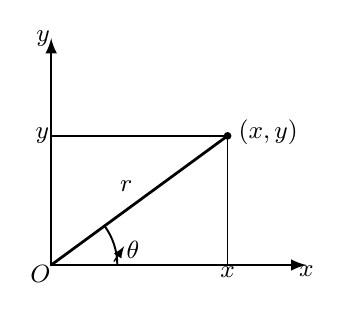
\begin{tikzpicture}[x=0.80cm, y=0.80cm, >=latex, line cap=round, line join=round]
  \draw[line width=0.9pt, ->] (0, 0) -- (4.05, 0) node[below=-1pt, inner sep=1pt] {\small $x$};
  \draw[line width=0.9pt, ->] (0, 0) -- (0, 3.60) node[left=-1pt, inner sep=1pt] {\small $y$};
  \node[below left=-1pt, inner sep=1pt] at (0, 0) {\small $O$};
  % 投影辅助线
  \draw[line width=0.6pt] (0, 2.05) -- (2.80, 2.05);
  \draw[line width=0.6pt] (2.80, 0) -- (2.80, 2.05);
  % 半径 r
  \draw[line width=1.0pt] (0, 0) -- (2.80, 2.05);
  \node[above left=-1pt, inner sep=1.5pt] at (1.32, 1.14) {\small $r$};
  % 夹角 theta
  \draw[line width=0.7pt] (1.05, 0) arc[start angle=0, end angle=36.2, radius=1.05];
  \draw[->, line width=0.5pt] (1.00, 0.06) -- (1.16, 0.30);
  \node[inner sep=1pt] at (1.30, 0.24) {\small $\theta$};
  % 端点
  \fill (2.80, 2.05) circle (1.4pt);
  \node[anchor=west, inner sep=1.5pt] at (2.90, 2.10) {\small $(x,y)$};
  \node[left=-1pt, inner sep=1.5pt] at (0, 2.05) {\small $y$};
  \node[below=-1pt, inner sep=1.5pt] at (2.80, 0) {\small $x$};
\end{tikzpicture}
\caption{}\label{fig:8.4.2}
\end{figure}

因此，$f$ 为局部 $C^{\infty}$ 微分同胚。但由 $f(1,0) = f(1,2\pi)$ 知 $f$ 非单射，从而整体的 $f^{-1}$ 不存在，$f$ 不为整体 $C^{\infty}$ 微分同胚。

再求 $r$，$\theta$ 关于 $x$，$y$ 的偏导数 $\dfrac{\partial r}{\partial x}$，$\dfrac{\partial r}{\partial y}$，$\dfrac{\partial\theta}{\partial x}$，$\dfrac{\partial\theta}{\partial y}$.
\end{example}

\begin{proof}[解法 1]
\begin{align*}
  \boldsymbol{J}f^{-1}(x,y) &= \bigl[\boldsymbol{J}f(\boldsymbol{r},\boldsymbol{\theta})\bigr]^{-1} \\
  &= \begin{pmatrix} \dfrac{\partial r}{\partial x} & \dfrac{\partial r}{\partial y} \\[6pt] \dfrac{\partial\theta}{\partial x} & \dfrac{\partial\theta}{\partial y} \end{pmatrix} = \begin{pmatrix} \dfrac{\partial x}{\partial r} & \dfrac{\partial x}{\partial\theta} \\[6pt] \dfrac{\partial y}{\partial r} & \dfrac{\partial y}{\partial\theta} \end{pmatrix}^{-1} = \begin{pmatrix} \cos\theta & -r\sin\theta \\ \sin\theta & r\cos\theta \end{pmatrix}^{-1} \\
  &= \frac{1}{r}\begin{pmatrix} r\cos\theta & r\sin\theta \\ -\sin\theta & \cos\theta \end{pmatrix} = \begin{pmatrix} \dfrac{x}{\sqrt{x^{2}+y^{2}}} & \dfrac{y}{\sqrt{x^{2}+y^{2}}} \\[8pt] -\dfrac{y}{x^{2}+y^{2}} & \dfrac{x}{x^{2}+y^{2}} \end{pmatrix}.
\end{align*}
\end{proof}

\begin{proof}[解法 2]
$r = \sqrt{x^{2}+y^{2}}$，$\theta = \arctan\dfrac{y}{x}$，因此
\[
  \frac{\partial r}{\partial x} = \frac{x}{\sqrt{x^{2}+y^{2}}},\quad \frac{\partial r}{\partial y} = \frac{y}{\sqrt{x^{2}+y^{2}}},
\]
\[
  \frac{\partial\theta}{\partial x} = \frac{-\dfrac{y}{x^{2}}}{1 + \left(\dfrac{y}{x}\right)^{2}} = -\frac{y}{x^{2}+y^{2}},\quad \frac{\partial\theta}{\partial y} = \frac{\dfrac{1}{x}}{1 + \left(\dfrac{y}{x}\right)^{2}} = \frac{x}{x^{2}+y^{2}}.
\]
\end{proof}

\begin{example}\label{ex:8.4.13}
设 $f: (0,+\infty) \times (0,\pi) \times (-\infty,+\infty) \to \mathbb{R}^{3}$，
\[
  (r,\theta,\varphi) \mapsto (x,y,z) = f(r,\theta,\varphi) = (r\sin\theta\cos\varphi,r\sin\theta\sin\varphi,r\cos\theta)
\]
为球坐标变换公式(图 8.4.3)，则
\begin{align*}
  \det \boldsymbol{J}f(\boldsymbol{r},\boldsymbol{\theta},\boldsymbol{\varphi}) &= \frac{\partial(x,y,z)}{\partial(r,\theta,\varphi)} = \begin{vmatrix} \dfrac{\partial x}{\partial r} & \dfrac{\partial x}{\partial\theta} & \dfrac{\partial x}{\partial\varphi} \\[6pt] \dfrac{\partial y}{\partial r} & \dfrac{\partial y}{\partial\theta} & \dfrac{\partial y}{\partial\varphi} \\[6pt] \dfrac{\partial z}{\partial r} & \dfrac{\partial z}{\partial\theta} & \dfrac{\partial z}{\partial\varphi} \end{vmatrix} \\
  &= \begin{vmatrix} \sin\theta\cos\varphi & r\cos\theta\cos\varphi & -r\sin\theta\sin\varphi \\ \sin\theta\sin\varphi & r\cos\theta\sin\varphi & r\sin\theta\cos\varphi \\ \cos\theta & -r\sin\theta & 0 \end{vmatrix} = r^{2}\sin\theta \neq 0.
\end{align*}

\begin{figure}[htbp]
\centering
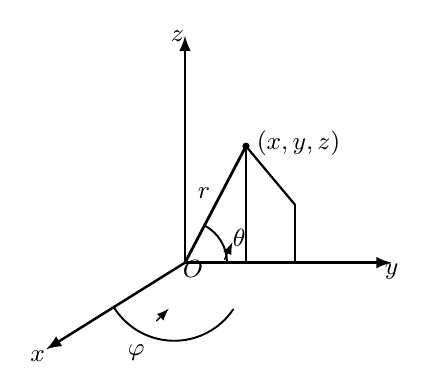
\begin{tikzpicture}[x=0.86cm, y=0.86cm, >=latex, line cap=round, line join=round]
  % 三轴
  \draw[line width=0.9pt, ->] (0, 0) -- (3.05, 0) node[below=-1pt, inner sep=1pt] {\small $y$};
  \draw[line width=0.9pt, ->] (0, 0) -- (0, 3.35) node[left=-1pt, inner sep=1pt] {\small $z$};
  \draw[line width=0.9pt, ->] (0, 0) -- (-2.05, -1.28) node[below left=-1pt, inner sep=1pt] {\small $x$};
  \node[below right=-2pt, inner sep=1pt] at (0, 0) {\small $O$};
  % 竖直投影三角形(母线)
  \draw[line width=0.8pt] (0.90, 0) -- (0.90, 1.72);
  \draw[line width=0.8pt] (0.90, 1.72) -- (1.62, 0.86);
  \draw[line width=0.8pt] (1.62, 0.86) -- (1.62, 0);
  % 半径 r
  \draw[line width=1.0pt] (0, 0) -- (0.90, 1.72);
  \node[above left=-1pt, inner sep=1.5pt] at (0.40, 0.92) {\small $r$};
  % theta 角
  \draw[line width=0.7pt] (0.62, 0) arc[start angle=0, end angle=62.4, radius=0.62];
  \draw[->, line width=0.5pt] (0.585, 0.05) -- (0.70, 0.30);
  \node[inner sep=1pt] at (0.80, 0.36) {\small $\theta$};
  % phi 角
  \draw[line width=0.7pt] (-1.05, -0.66) arc[start angle=212, end angle=326, radius=1.05];
  \draw[->, line width=0.5pt] (-0.42, -0.86) -- (-0.24, -0.68);
  \node[below=-1pt, inner sep=1pt] at (-0.72, -1.20) {\small $\varphi$};
  % 点 (x,y,z)
  \fill (0.90, 1.72) circle (1.3pt);
  \node[anchor=west, inner sep=1.5pt] at (0.99, 1.76) {\small $(x,y,z)$};
\end{tikzpicture}
\caption{}\label{fig:8.4.3}
\end{figure}

因此，$f$ 为局部 $C^{\infty}$ 微分同胚。但由 $f\left(1,\dfrac{\pi}{2},0\right) = f\left(1,\dfrac{\pi}{2},2\pi\right)$ 知，$f$ 非单射，从而整体的 $f^{-1}$ 不存在，$f$ 不为整体的 $C^{\infty}$ 微分同胚。
\end{example}

\begin{proof}[解法 1]
\begin{align*}
  \boldsymbol{J}f^{-1}(x,y,z) &= \bigl[\boldsymbol{J}f(\boldsymbol{r},\boldsymbol{\theta},\boldsymbol{\varphi})\bigr]^{-1} \\
  &= \begin{pmatrix} \dfrac{\partial r}{\partial x} & \dfrac{\partial r}{\partial y} & \dfrac{\partial r}{\partial z} \\[6pt] \dfrac{\partial\theta}{\partial x} & \dfrac{\partial\theta}{\partial y} & \dfrac{\partial\theta}{\partial z} \\[6pt] \dfrac{\partial\varphi}{\partial x} & \dfrac{\partial\varphi}{\partial y} & \dfrac{\partial\varphi}{\partial z} \end{pmatrix} \\
  &= \begin{pmatrix} \dfrac{\partial x}{\partial r} & \dfrac{\partial x}{\partial\theta} & \dfrac{\partial x}{\partial\varphi} \\[6pt] \dfrac{\partial y}{\partial r} & \dfrac{\partial y}{\partial\theta} & \dfrac{\partial y}{\partial\varphi} \\[6pt] \dfrac{\partial z}{\partial r} & \dfrac{\partial z}{\partial\theta} & \dfrac{\partial z}{\partial\varphi} \end{pmatrix}^{-1} \\
  &= \begin{pmatrix} \sin\theta\cos\varphi & r\cos\theta\cos\varphi & -r\sin\theta\sin\varphi \\ \sin\theta\sin\varphi & r\cos\theta\sin\varphi & r\sin\theta\cos\varphi \\ \cos\theta & -r\sin\theta & 0 \end{pmatrix}^{-1} \\
  &= \frac{1}{r^{2}\sin\theta}\begin{pmatrix} r^{2}\sin^{2}\theta\cos\varphi & r^{2}\sin^{2}\theta\sin\varphi & r^{2}\sin\theta\cos\theta \\ r\sin\theta\cos\theta\cos\varphi & r\sin\theta\cos\theta\sin\varphi & -r\sin^{2}\theta \\ -r\sin\varphi & r\cos\varphi & 0 \end{pmatrix} \\
  &= \begin{pmatrix} \sin\theta\cos\varphi & \sin\theta\sin\varphi & \cos\theta \\[4pt] \dfrac{\cos\theta\cos\varphi}{r} & \dfrac{\cos\theta\sin\varphi}{r} & -\dfrac{\sin\theta}{r} \\[8pt] -\dfrac{\sin\varphi}{r\sin\theta} & \dfrac{\cos\varphi}{r\sin\theta} & 0 \end{pmatrix} \\
  &= \begin{pmatrix} \dfrac{x}{r} & \dfrac{y}{r} & \dfrac{z}{r} \\[8pt] \dfrac{xz}{r^{2}\sqrt{x^{2}+y^{2}}} & \dfrac{yz}{r^{2}\sqrt{x^{2}+y^{2}}} & -\dfrac{\sqrt{x^{2}+y^{2}}}{r^{2}} \\[8pt] -\dfrac{y}{x^{2}+y^{2}} & \dfrac{x}{x^{2}+y^{2}} & 0 \end{pmatrix},
\end{align*}
其中 $x^{2}+y^{2} = r^{2}\sin^{2}\theta \neq 0$，$r = \sqrt{x^{2}+y^{2}+z^{2}} \neq 0$，
\[
  r = \sqrt{x^{2}+y^{2}+z^{2}},\quad \theta = \arccos\frac{z}{\sqrt{x^{2}+y^{2}+z^{2}}},\quad \varphi = \arcsin\frac{y}{\sqrt{x^{2}+y^{2}}}.
\]
通过简单计算，分别求出 $r$，$\theta$，$\varphi$ 对于 $x$，$y$，$z$ 的偏导数可以验证与上述结果完全一致.
\end{proof}

\begin{example}\label{ex:8.4.14}
设 $U \subset \mathbb{R}^{4}$ 为开集，$F$，$G: U \to \mathbb{R}^{1}$ 为 4 元函数。如果 $\boldsymbol{H} = (F,G)^{\mathrm{T}}$ 在点 $(z_{0},w_{0}) \in U$ (其中 $z_{0} = (x_{0},y_{0})$，$w_{0} = (u_{0},v_{0})$) 的某开邻域内满足隐射定理 8.4.2 的条件且 $\det \boldsymbol{J}_{w}H(z_{0},w_{0}) \neq 0$，则方程组 $\boldsymbol{H}(x,y,u,v) = \boldsymbol{0}$ 在点 $z_{0}$ 的某开邻域内能确定一个 $C^{k}$ 隐映 $w = f(z)$.
\end{example}

\begin{proof}[解法 1]
由定理 8.4.2 中的 (4) 求得
\[
  \boldsymbol{J}f(\boldsymbol{z}) = -\bigl[\boldsymbol{J}_{w}\boldsymbol{H}(\boldsymbol{z},\boldsymbol{w})\bigr]^{-1}\boldsymbol{J}_{z}\boldsymbol{H}(\boldsymbol{z},\boldsymbol{w}),
\]
即
\[
  \begin{pmatrix} \dfrac{\partial u}{\partial x} & \dfrac{\partial u}{\partial y} \\[6pt] \dfrac{\partial v}{\partial x} & \dfrac{\partial v}{\partial y} \end{pmatrix} = -\begin{pmatrix} \dfrac{\partial F}{\partial u} & \dfrac{\partial F}{\partial v} \\[6pt] \dfrac{\partial G}{\partial u} & \dfrac{\partial G}{\partial v} \end{pmatrix}^{-1}\begin{pmatrix} \dfrac{\partial F}{\partial x} & \dfrac{\partial F}{\partial y} \\[6pt] \dfrac{\partial G}{\partial x} & \dfrac{\partial G}{\partial y} \end{pmatrix}
\]
\begin{align*}
  &= -\frac{-1}{J}\begin{pmatrix} \dfrac{\partial G}{\partial v} & -\dfrac{\partial F}{\partial v} \\[6pt] -\dfrac{\partial G}{\partial u} & \dfrac{\partial F}{\partial u} \end{pmatrix}\begin{pmatrix} \dfrac{\partial F}{\partial x} & \dfrac{\partial F}{\partial y} \\[6pt] \dfrac{\partial G}{\partial x} & \dfrac{\partial G}{\partial y} \end{pmatrix} \\
  &= -\frac{1}{J}\begin{pmatrix} \dfrac{\partial(F,G)}{\partial(x,v)} & \dfrac{\partial(F,G)}{\partial(y,v)} \\[6pt] \dfrac{\partial(F,G)}{\partial(u,x)} & \dfrac{\partial(F,G)}{\partial(u,y)} \end{pmatrix},
\end{align*}
其中 $J = \dfrac{\partial(F,G)}{\partial(u,v)}$.
\end{proof}

\begin{proof}[解法 2]
设 $u = f(x,y)$，$v = g(x,y)$ 为由方程组
\[
  \left\{\begin{aligned}
    F(x,y,u,v) &= 0, \\
    G(x,y,u,v) &= 0
  \end{aligned}\right.
\]
所确定的隐函数，即
\[
  \left\{\begin{aligned}
    F(x,y,f(x,y),g(x,y)) &\equiv 0, \\
    G(x,y,f(x,y),g(x,y)) &\equiv 0.
  \end{aligned}\right.
\]
对上述方程组关于 $x$，$y$ 分别求偏导数得到
\begin{align*}
  &\left\{\begin{aligned}
    F_{x}^{\prime} + F_{u}^{\prime}u_{x}^{\prime} + F_{v}^{\prime}v_{x}^{\prime} &= 0, \\
    G_{x}^{\prime} + G_{u}^{\prime}u_{x}^{\prime} + G_{v}^{\prime}v_{x}^{\prime} &= 0,
  \end{aligned}\right. \\
  &\left\{\begin{aligned}
    F_{y}^{\prime} + F_{u}^{\prime}u_{y}^{\prime} + F_{v}^{\prime}v_{y}^{\prime} &= 0, \\
    G_{y}^{\prime} + G_{u}^{\prime}u_{y}^{\prime} + G_{v}^{\prime}v_{y}^{\prime} &= 0.
  \end{aligned}\right.
\end{align*}
因为
\[
  J = \frac{\partial(F,G)}{\partial(u,v)} = \begin{vmatrix} F_{u}^{\prime} & F_{v}^{\prime} \\ G_{u}^{\prime} & G_{v}^{\prime} \end{vmatrix} \neq 0,
\]
故从两个方程组分别解得
\[
  \frac{\partial u}{\partial x} = u_{x}^{\prime} = -\frac{1}{J}\frac{\partial(F,G)}{\partial(x,v)},\quad \frac{\partial u}{\partial y} = u_{y}^{\prime} = -\frac{1}{J}\frac{\partial(F,G)}{\partial(y,v)},
\]
\[
  \frac{\partial v}{\partial x} = v_{x}^{\prime} = -\frac{1}{J}\frac{\partial(F,G)}{\partial(u,x)},\quad \frac{\partial v}{\partial y} = v_{y}^{\prime} = -\frac{1}{J}\frac{\partial(F,G)}{\partial(u,y)}.
\]
\end{proof}

\begin{exblock}{练习题 8.4}
\item 下列方程确定隐函数 $y = y(x)$，计算 $\dfrac{\mathrm{d}y}{\mathrm{d}x}$;
\begin{enumerate}
  \item[(1)] $x^{2} + 2xy - y^{2} = a^{2}$;
  \item[(2)] $xy - \ln y = 0$，在点 $(0,1)$ 处;
  \item[(3)] $y - \varepsilon \sin y = x$，常数 $\varepsilon \in (0,1)$;
  \item[(4)] $x^{y} = y^{x}$
\end{enumerate}

\item 下列方程确定隐函数 $z = z(x,y)$，计算 $\dfrac{\partial z}{\partial x}$ 与 $\dfrac{\partial z}{\partial y}$.
\begin{enumerate}
  \item[(1)] $e^{x} - xyz = 0$;
  \item[(2)] $\dfrac{x}{z} = \ln\dfrac{z}{y}$;
  \item[(3)] $x + y + z = e^{-(x+y+z)}$，并对计算的结果作出解释;
  \item[(4)] $z^{2}y - xz^{3} - 1 = 0$，在点 $(1,2,1)$ 处.
\end{enumerate}

\item 设 $u = f(x,y,z,t)$，$g(y,z,t) = 0$，$h(z,t) = 0$，$f$，$g$ 与 $h$ 都一阶连续可导，计算 $\dfrac{\partial u}{\partial x}$ 与 $\dfrac{\partial u}{\partial y}$，并给出相应可计算的条件.

\item 设 $F(x-y,y-z,z-x) = 0$，$F$ 有一阶连续偏导数，计算 $\dfrac{\partial z}{\partial x}$ 与 $\dfrac{\partial z}{\partial y}$，并给出相应可计算的条件.

\item 设 $F(x+y+z,x^{2}+y^{2}+z^{2}) = 0$，$F$ 有一阶连续偏导数，计算 $\dfrac{\partial z}{\partial x}$ 与 $\dfrac{\partial z}{\partial y}$，并给出相应可计算的条件.

\item 二元函数 $F$ 在 $\mathbb{R}^{2}$ 上二次连续可导. 已知曲线 $F(x,y) = 0$ 呈“8”字形. 问方程组
\[
  \begin{cases}
    \dfrac{\partial F}{\partial x}(x,y) = 0, \\[4pt]
    \dfrac{\partial F}{\partial y}(x,y) = 0
  \end{cases}
\]
在 $\mathbb{R}^{2}$ 中至少有几组解?

\item 从方程组
\[
  \left\{\begin{aligned}
    x^{2} + y^{2} + z^{2} &= 1, \\
    x + y + z &= 0
  \end{aligned}\right.
\]
中，计算 $\dfrac{\mathrm{d}y}{\mathrm{d}x}$ 与 $\dfrac{\mathrm{d}z}{\mathrm{d}x}$，并作出几何解释.

\item 从方程组
\[
  \left\{\begin{aligned}
    x^{2} + y^{2} - z &= 0, \\
    x^{2} + 2y^{2} + 3z^{2} &= 20
  \end{aligned}\right.
\]
中，计算 $\dfrac{\mathrm{d}y}{\mathrm{d}x}$ 与 $\dfrac{\mathrm{d}z}{\mathrm{d}x}$，并作出几何解释.

\item 从下列方程中，计算 Jacobi 矩阵
\[
  \begin{pmatrix} \dfrac{\partial x}{\partial u} & \dfrac{\partial x}{\partial v} \\[6pt] \dfrac{\partial y}{\partial u} & \dfrac{\partial y}{\partial v} \end{pmatrix}.
\]
\begin{enumerate}
  \item[(1)] $xu - yv = 0$，$yu + xv = 1$;
  \item[(2)] $x + y = u + v$，$\dfrac{x}{y} = \dfrac{\sin u}{\sin v}$.
\end{enumerate}

\item 设
\[
  \left\{\begin{aligned}
    u^{2} - v\cos(xy) + w^{2} &= 0, \\
    u^{2} + v^{2} - \sin(xy) + 2w^{2} &= 2, \\
    uv - \sin x \cos y + w &= 0,
  \end{aligned}\right.
\]
试在 $(x,y) = \left(\dfrac{\pi}{2},0\right)$，$(u,v,w) = (1,1,0)$ 处计算 Jacobi 矩阵
\[
  \begin{pmatrix} \dfrac{\partial u}{\partial x} & \dfrac{\partial u}{\partial y} \\[6pt] \dfrac{\partial v}{\partial x} & \dfrac{\partial v}{\partial y} \\[6pt] \dfrac{\partial w}{\partial x} & \dfrac{\partial w}{\partial y} \end{pmatrix}.
\]

\item 从方程组
\[
  \left\{\begin{aligned}
    x &= t + \dfrac{1}{t}, \\
    y &= t^{2} + \dfrac{1}{t^{2}}, \\
    z &= t^{3} + \dfrac{1}{t^{3}}
  \end{aligned}\right.
\]
中，计算 $\dfrac{\mathrm{d}y}{\mathrm{d}x}$ 与 $\dfrac{\mathrm{d}z}{\mathrm{d}x}$.

\item 设 $U \subset \mathbb{R}^{n}$，$f: U \to \mathbb{R}^{n}$. 如果 $f$ 将开集映为开集，则称 $f$ 为一个开映射。问: 下列映射是否为开映射? 并说明理由。
\begin{enumerate}
  \item[(1)] $f(x,y) = \left(x^{2},\dfrac{y}{x}\right)$;
  \item[(2)] $f(x,y) = \left(\mathrm{e}^{x}\cos y,\mathrm{e}^{x}\sin y\right)$;
  \item[(3)] $f(x,y) = (x,x^{2})$
\end{enumerate}
进而，对 (1) 与 (2) 中的 $f$，计算 $\boldsymbol{J}f^{-1}$

\item 求由下列方程所确定的隐函数的偏导数:
\begin{enumerate}
  \item[(1)] $x + y + z = \mathrm{e}^{-(x+y+z)}$，求 $z$ 对 $x$，$y$ 的一阶与二阶偏导数;
  \item[(2)] $F(x,x+y,x+y+z) = 0$，$F$ 为 $C^{2}$ 函数，求 $\dfrac{\partial z}{\partial x}$，$\dfrac{\partial z}{\partial y}$，$\dfrac{\partial^{2} z}{\partial x^{2}}$.
\end{enumerate}

\item 设 $f$ 为一元函数，试问: $f$ 应满足什么条件，方程 $2f(xy) = f(x) + f(y)$ 在点 $(1,1)$ 的开邻域内能确定出惟一的 $y$ 为 $x$ 的函数?

\item 设 $F(x,y)$ 为 $C^{2}$ 函数，$F_{y}^{\prime} \neq 0$，证明: 由 $F(x,y) = 0$ 所确定的隐函数 $y = f(x)$ 有
\[
  \left(F_{y}^{\prime}\right)^{3} y'' = \begin{vmatrix} F_{xx}^{\prime\prime} & F_{xy}^{\prime\prime} & F_{x}^{\prime} \\ F_{xy}^{\prime\prime} & F_{yy}^{\prime\prime} & F_{y}^{\prime} \\ F_{x}^{\prime} & F_{y}^{\prime} & 0 \end{vmatrix}.
\]

\item 求由下列方程所确定的隐函数的极值:
\begin{enumerate}
  \item[(1)] $x^{2} + 2xy + 2y^{2} = 1$
  \item[(2)] $(x^{2}+y^{2}) = a^{2}(x^{2}-y^{2})$ $(a > 0)$
\end{enumerate}

\item 设 $f$，$g$，$h$ 可微，
\[
  \begin{cases}
    x = f(u,v,w), \\
    y = g(u,v,w), \\
    z = h(u,v,w),
  \end{cases}
\]
求 $\dfrac{\partial u}{\partial x}$，$\dfrac{\partial u}{\partial y}$，$\dfrac{\partial u}{\partial z}$，并给出可计算的条件.

\item 设 $f$，$g$ 为可微函数，求下列方程所确定的隐函数 $u = u(x,y)$ 的偏导数 $\dfrac{\partial u}{\partial x}$，$\dfrac{\partial u}{\partial y}$
\begin{enumerate}
  \item[(1)] $x^{2} + u^{2} = f(x,u) + g(x,y,u)$;
  \item[(2)] $u = f(x + u,yu)$.
\end{enumerate}
进而给出可计算的条件.

\item 设 $y = f(x)$ 为 $C^{1}$ 函数，$x = \varphi(u,v)$，$y = \psi(u,v)$ 为 $C^{2}$ 函数，则由方程 $\psi(u,v) = f(\varphi(u,v))$ 可以确定函数 $v = v(u)$. 试用 $u$，$v$，$\dfrac{\mathrm{d}v}{\mathrm{d}u}$，$\dfrac{\mathrm{d}^{2}v}{\mathrm{d}u^{2}}$ 表示 $\dfrac{\mathrm{d}y}{\mathrm{d}x}$，$\dfrac{\mathrm{d}^{2}y}{\mathrm{d}x^{2}}$; 并给出可计算的条件.
\end{exblock}

\begin{exblock}{思考题 8.4}
\item 设 $(x_{0},y_{0},z_{0},u_{0})$ 满足方程组
\[
  \left\{\begin{aligned}
    f(x) + f(y) + f(z) &= F(u), \\
    g(x) + g(y) + g(z) &= G(u), \\
    h(x) + h(y) + h(z) &= H(u),
  \end{aligned}\right.
\]
这里所有的函数假定有连续的导数.

(1) 说出一个能在该点开邻域内确定 $x$，$y$，$z$ 为 $u$ 的函数的充分条件;

(2) 在 $f(x) = x$，$g(x) = x^{2}$，$h(x) = x^{3}$ 的情形下，上述条件相当于什么?

\item 据理说明: 在点 $(0,1)$ 近旁是否存在 $C^{\infty}$ 的 $f(x,y)$ 与 $g(x,y)$ 满足:
\[
  f(0,1) = 1,\quad g(0,1) = -1,
\]
且
\[
  \left\{\begin{aligned}
    [f(x,y)]^{3} + x g(x,y) - y &= 0, \\
    [g(x,y)]^{3} + y f(x,y) - x &= 0.
  \end{aligned}\right.
\]
\end{exblock}


\section{逆射与隐射定理的另一精美证法}\label{sec:8.5}

上节应用数学归纳法先证隐射定理: 方程组 $F(x,y) = 0$ 在条件 $\det J_{y}F \neq 0$ 时, 局部解得 $y = f(x)$, 使得 $F(x,f(x)) \equiv 0$. 进而, 当 $\det Jf(x) \neq 0$ 时, 对 $F(x,y) = f(x) - y = 0$ 施用隐射定理, 证得 $y = f(x)$ 有局部逆射 $x = g(y) = f^{-1}(y)$. 读者已领略了它的精美的论证方法. 自然会大胆地问: 能否先证局部逆射定理, 再应用局部逆射定理来证明隐射定理? 现在来实现这一设想.

\begin{theorem}[局部逆射定理]\label{thm:8.5.1}
设 $D \subset \mathbb{R}^{n}$ 为开集, $f: D \to \mathbb{R}^{n}$ 为 $C^{k}$ $(1 \leqslant k \leqslant +\infty)$ 映射, 且
\[
  \det Jf(\boldsymbol{x}^{0}) = \det\left(\frac{\partial f_{i}}{\partial x_{j}}(\boldsymbol{x}^{0})\right) \neq 0, \quad \boldsymbol{x}^{0} \in D,
\]
则 $f$ 为一个 $C^{k}$ 局部微分同胚, 它将 $\boldsymbol{x}^{0}$ 的一个开邻域映成 $f(\boldsymbol{x}^{0})$ 的一个开邻域.
\end{theorem}

\begin{proof}
可以假定 $\boldsymbol{x}^{0} = \boldsymbol{0}$, $f(\boldsymbol{x}^{0}) = \boldsymbol{0}$, $\left(\dfrac{\partial f_{i}}{\partial x_{j}}(\boldsymbol{x}^{0})\right) = (\delta_{j}^{i}) = \boldsymbol{I}$ (否则作一仿射变换, 不影响定理的证明). 选 $a$ 充分小, 使得方体
\[
  C^{n}(a) = \bigl\{\boldsymbol{x} \in \mathbb{R}^{n} \mid \|\boldsymbol{x}\| = \max_{1 \leqslant j \leqslant n}|x_{j}| < a\bigr\} \subset D,
\]
且当 $\boldsymbol{x} \in C^{n}(a)$ 时,
\[
  \det\left(\frac{\partial f_{i}}{\partial x_{j}}(\boldsymbol{x})\right) \neq 0
\]
及
\[
  \left(\frac{\partial f_{i}}{\partial x_{j}}(\boldsymbol{x})\right) - \boldsymbol{I}
\]
中的元素满足
\[
  \left|\left(\frac{\partial f_{i}}{\partial x_{j}}(\boldsymbol{x})\right) - \delta_{j}^{i}\right| \leqslant \frac{1}{2n}
  \quad \biggl(\text{只需注意}\ \left(\frac{\partial f_{i}}{\partial x_{j}}(\boldsymbol{0})\right) - \boldsymbol{I} = \boldsymbol{0}\biggr).
\]
令 $g(\boldsymbol{x}) = f(\boldsymbol{x}) - \boldsymbol{x}$, 则当 $\boldsymbol{x}^{1}, \boldsymbol{x}^{2} \in C^{n}(a)$ 时, 应用 Lagrange 中值定理有
\begin{align*}
  \|\boldsymbol{g}(\boldsymbol{x}^{1}) - \boldsymbol{g}(\boldsymbol{x}^{2})\| &= \max_{1 \leqslant i \leqslant n}\bigl\{|g_{i}(\boldsymbol{x}^{1}) - g_{i}(\boldsymbol{x}^{2})|\bigr\} \\
  &= \max_{1 \leqslant i \leqslant n}\left\{\left|\sum_{j=1}^{n}\frac{\partial g_{i}}{\partial x_{j}}(\boldsymbol{\xi}^{j})(x_{j}^{1} - x_{j}^{2})\right|\right\} \\
  &\leqslant n\max_{1 \leqslant i, j \leqslant n}\left\{\left|\frac{\partial g_{i}}{\partial x_{j}}(\boldsymbol{\xi}^{j})\right|\right\}\max_{1 \leqslant j \leqslant n}\bigl\{|x_{j}^{1} - x_{j}^{2}|\bigr\} \\
  &\leqslant n \cdot \frac{1}{2n}\|\boldsymbol{x}^{1} - \boldsymbol{x}^{2}\| = \frac{1}{2}\|\boldsymbol{x}^{1} - \boldsymbol{x}^{2}\|.
\end{align*}
此外, 还有
\begin{align*}
  \|f(\boldsymbol{x}^{1}) - f(\boldsymbol{x}^{2})\| &= \|\boldsymbol{g}(\boldsymbol{x}^{1}) - \boldsymbol{g}(\boldsymbol{x}^{1}) + \boldsymbol{x}^{1} - \boldsymbol{x}^{2}\| \\
  &\geqslant \|\boldsymbol{x}^{1} - \boldsymbol{x}^{2}\| - \|\boldsymbol{g}(\boldsymbol{x}^{1}) - \boldsymbol{g}(\boldsymbol{x}^{2})\| \\
  &\geqslant \|\boldsymbol{x}^{1} - \boldsymbol{x}^{2}\| - \frac{1}{2}\|\boldsymbol{x}^{1} - \boldsymbol{x}^{2}\| \\
  &= \frac{1}{2}\|\boldsymbol{x}^{1} - \boldsymbol{x}^{2}\|.
\end{align*}
\begin{enumerate}
\item[(1)] 如果 $\boldsymbol{y} \in C^{n}\left(\dfrac{a}{2}\right)$, 则必存在一点 $\boldsymbol{x} \in C^{n}(a)$, 使得 $f(\boldsymbol{x}) = \boldsymbol{y}$.

为此, 设
\[
  \boldsymbol{x}^{0} = \boldsymbol{0}, \quad \boldsymbol{x}^{1} = \boldsymbol{y}, \quad \boldsymbol{x}^{k+1} = \boldsymbol{y} - \boldsymbol{g}(\boldsymbol{x}^{k}), \quad k = 0, 1, 2, \cdots,
\]
容易看出
\begin{align*}
  \|\boldsymbol{x}^{k} - \boldsymbol{x}^{k-1}\| &= \|\boldsymbol{g}(\boldsymbol{x}^{k-1}) - \boldsymbol{g}(\boldsymbol{x}^{k-2})\| \leqslant \frac{1}{2}\|\boldsymbol{x}^{k-1} - \boldsymbol{x}^{k-2}\| \\
  \leqslant {} & \cdots \leqslant \frac{1}{2^{k-2}}\|\boldsymbol{x}^{1} - \boldsymbol{x}^{0}\| = \frac{1}{2^{k-1}}\|\boldsymbol{y}\|,
\end{align*}
\begin{align*}
  \|\boldsymbol{x}^{k}\| &= \|\boldsymbol{x}^{k} - \boldsymbol{x}^{0}\| \\
  &\leqslant \|\boldsymbol{x}^{k} - \boldsymbol{x}^{k-1}\| + \|\boldsymbol{x}^{k-1} - \boldsymbol{x}^{k-2}\| + \cdots + \|\boldsymbol{x}^{1} - \boldsymbol{x}^{0}\| \\
  &\leqslant \left(\frac{1}{2^{k-1}} + \frac{1}{2^{k-2}} + \cdots + 1\right)\|\boldsymbol{y}\| < 2\|\boldsymbol{y}\| < 2 \cdot \frac{a}{2} = a,
\end{align*}
\begin{align*}
  \|\boldsymbol{x}^{k+p} - \boldsymbol{x}^{k}\| &\leqslant \|\boldsymbol{x}^{k+p} - \boldsymbol{x}^{k+p-1}\| + \cdots + \|\boldsymbol{x}^{k+1} - \boldsymbol{x}^{k}\| \\
  &\leqslant \left(\frac{1}{2^{k+p-1}} + \cdots + \frac{1}{2^{k}}\right)\|\boldsymbol{y}\| \\
  &= \frac{1}{2^{k}}\left(\frac{1}{2^{p-1}} + \cdots + 1\right)\|\boldsymbol{y}\| \leqslant \frac{1}{2^{k-1}}\|\boldsymbol{y}\|.
\end{align*}
于是, $\boldsymbol{x}^{k} \in C^{n}(a)$ 及 $\{\boldsymbol{x}^{k}\}$ 为 Cauchy 点列. 由于 $\mathbb{R}^{n}$ 完备, 故 $\{\boldsymbol{x}^{k}\}$ 收敛, 设 $\lim\limits_{k \to +\infty}\boldsymbol{x}^{k} = \boldsymbol{x}$, 再在上述第二个不等式中令 $k \to +\infty$ 得到
\[
  \|\boldsymbol{x}\| < 2\|\boldsymbol{y}\| < a,
\]
因而 $\boldsymbol{x} \in C^{n}(a)$, 且
\begin{align*}
  \boldsymbol{x} &= \lim_{k \to +\infty}\boldsymbol{x}^{k+1} = \lim_{k \to +\infty}\bigl[\boldsymbol{y} - \boldsymbol{g}(\boldsymbol{x}^{k})\bigr] = \boldsymbol{y} - \boldsymbol{g}(\boldsymbol{x}) \\
  &= \boldsymbol{y} - \bigl[f(\boldsymbol{x}) - \boldsymbol{x}\bigr] = \boldsymbol{y} - f(\boldsymbol{x}) + \boldsymbol{x}, \quad f(\boldsymbol{x}) = \boldsymbol{y}.
\end{align*}
这就证明了 $\boldsymbol{x}$ 的存在性.

再证惟一性. 如果 $\exists\,\boldsymbol{x}, \boldsymbol{x}' \in C^{n}(a)$, s. t.\ $f(\boldsymbol{x}) = \boldsymbol{y} = f(\boldsymbol{x}')$, 则由
\[
  0 = \|f(\boldsymbol{x}) - f(\boldsymbol{x}')\| \geqslant \frac{1}{2}\|\boldsymbol{x} - \boldsymbol{x}'\| \geqslant 0,
\]
推得 $\|\boldsymbol{x} - \boldsymbol{x}'\| = 0$, $\boldsymbol{x} = \boldsymbol{x}'$.

\item[(2)] 由 (1) 知 $f^{-1}: C^{n}\left(\dfrac{a}{2}\right) \to C^{n}(a)$ 是存在的. 另一方面, 从
\[
  \|\boldsymbol{y}' - \boldsymbol{y}''\| = \|f(\boldsymbol{x}') - f(\boldsymbol{x}'')\| \geqslant \frac{1}{2}\|\boldsymbol{x}' - \boldsymbol{x}''\| = \frac{1}{2}\|f^{-1}(\boldsymbol{y}') - f^{-1}(\boldsymbol{y}'')\|
\]
可推出 $f^{-1}$ 在 $C^{n}\left(\dfrac{a}{2}\right)$ 上是一致连续的, 因而是连续的.

显然, 由 $f$ 连续及 $C^{n}\left(\dfrac{a}{2}\right)$ 为开集知, $f^{-1}\left(C^{n}\left(\dfrac{a}{2}\right)\right)$ 为开集, 从而 $C^{n}\left(\dfrac{a}{2}\right)$ 在 $f^{-1}: C^{n}\left(\dfrac{a}{2}\right) \to C^{n}(a)$ 下的逆像为 $C^{n}(a) \cap f^{-1}\left(C^{n}\left(\dfrac{a}{2}\right)\right)$, 它是开集. 这就证明了
\[
  f: C^{n}(a) \cap f^{-1}\left(C^{n}\left(\frac{a}{2}\right)\right) \to C^{n}\left(\frac{a}{2}\right)
\]
为一个同胚 (拓扑映射), 它将 $\boldsymbol{0}$ 的一个开邻域映成 $f(\boldsymbol{0}) = \boldsymbol{0}$ 的一个开邻域.

\item[(3)] $f^{-1}$ 是可微的, 由此得到 $J(f^{-1})$ 是存在的.

由于 $f$ 是 $C^{k}$ $(1 \leqslant k \leqslant +\infty)$, 根据\cref{thm:8.2.4}, $f$ 在 $\forall\,\boldsymbol{x}^{1} \in C^{n}(a) \cap f^{-1}\left(C^{n}\left(\dfrac{a}{2}\right)\right)$ 是可微的, 即
\[
  f(\boldsymbol{x}) - f(\boldsymbol{x}') = \left(\frac{\partial f_{i}}{\partial x_{j}}(\boldsymbol{x}^{1})\right)(\boldsymbol{x} - \boldsymbol{x}^{1}) + \boldsymbol{h}(\boldsymbol{x}^{1}, \boldsymbol{x}),
\]
\[
  \lim_{\|\boldsymbol{x} - \boldsymbol{x}^{1}\| \to 0}\frac{\boldsymbol{h}(\boldsymbol{x}^{1}, \boldsymbol{x})}{\|\boldsymbol{x} - \boldsymbol{x}^{1}\|} = 0
  \quad (\boldsymbol{x}^{1}\ \text{固定}), \quad \boldsymbol{x}^{1}, \boldsymbol{x} \in C^{n}(a) \cap \boldsymbol{f}^{-1}\left(C^{n}\left(\frac{a}{2}\right)\right).
\]
记 $\left(\dfrac{\partial f_{i}}{\partial x_{j}}(\boldsymbol{x}^{1})\right)^{-1}$ 为 $\left(\dfrac{\partial f_{i}}{\partial x_{j}}(\boldsymbol{x}^{1})\right)$ 的逆矩阵, 则
\[
  \left(\frac{\partial f_{i}}{\partial x_{j}}(\boldsymbol{x}^{1})\right)^{-1}\bigl[\boldsymbol{f}(\boldsymbol{x}) - \boldsymbol{f}(\boldsymbol{x}^{1})\bigr] = (\boldsymbol{x} - \boldsymbol{x}^{1}) + \left(\frac{\partial f_{i}}{\partial x_{j}}(\boldsymbol{x}^{1})\right)^{-1}\boldsymbol{h}(\boldsymbol{x}^{1}, \boldsymbol{x}),
\]
\[
  \left(\frac{\partial f_{i}}{\partial x_{j}}(\boldsymbol{x}^{1})\right)^{-1}(\boldsymbol{y} - \boldsymbol{y}^{1}) + \tilde{\boldsymbol{h}}(\boldsymbol{y}^{1}, \boldsymbol{y}) = \boldsymbol{f}^{-1}(\boldsymbol{y}) - \boldsymbol{f}^{-1}(\boldsymbol{y}^{1}),
\]
其中 $\tilde{\boldsymbol{h}}(\boldsymbol{y}^{1}, \boldsymbol{y}) = -\left(\dfrac{\partial f_{i}}{\partial x_{j}}(\boldsymbol{x}^{1})\right)^{-1}\boldsymbol{h}(\boldsymbol{x}^{1}, \boldsymbol{x})$. 因为
\[
  \|\boldsymbol{y} - \boldsymbol{y}^{1}\| = \|f(\boldsymbol{x}) - f(\boldsymbol{x}^{1})\| \geqslant \frac{1}{2}\|\boldsymbol{x} - \boldsymbol{x}^{1}\|,
\]
\[
  \frac{\|\boldsymbol{x} - \boldsymbol{x}^{1}\|}{\|\boldsymbol{y} - \boldsymbol{y}^{1}\|} \leqslant 2, \quad \|\boldsymbol{y} - \boldsymbol{y}^{1}\| \neq 0,
\]
所以,
\begin{align*}
  \lim_{\boldsymbol{y} \to \boldsymbol{y}^{1}}\frac{\tilde{\boldsymbol{h}}(\boldsymbol{y}^{1}, \boldsymbol{y})}{\|\boldsymbol{y} - \boldsymbol{y}^{1}\|} &= \lim_{\boldsymbol{y} \to \boldsymbol{y}^{1}}\frac{-\left(\frac{\partial f_{i}}{\partial x_{j}}(\boldsymbol{x}^{1})\right)^{-1}\boldsymbol{h}(f^{-1}(\boldsymbol{y}^{1}), f^{-1}(\boldsymbol{y}))}{\|\boldsymbol{y} - \boldsymbol{y}^{1}\|} \\
  &= -\left(\frac{\partial f_{i}}{\partial x_{j}}(\boldsymbol{x}^{1})\right)^{-1}\lim_{\boldsymbol{x} \to \boldsymbol{x}^{1}}\frac{\boldsymbol{h}(\boldsymbol{x}^{1}, \boldsymbol{x})}{\|\boldsymbol{x} - \boldsymbol{x}^{1}\|} \cdot \frac{\|\boldsymbol{x} - \boldsymbol{x}^{1}\|}{\|\boldsymbol{y} - \boldsymbol{y}^{1}\|} = \boldsymbol{0}.
\end{align*}
{\emergencystretch=3em 这就证明了 $f^{-1}$ 在 $\boldsymbol{y}^{1}$ 是可微的. 根据\cref{thm:8.2.3} 可推出 $(f^{-1})_{i}$ 在 $\boldsymbol{y}^{1}$ 有关于 $y_{1}, y_{2}, \cdots, y_{n}$ 的偏导数, 且\par}
\[
  \left(\frac{\partial (f^{-1})_{i}}{\partial y_{j}}(\boldsymbol{y}^{1})\right) = \left(\frac{\partial f_{i}}{\partial x_{j}}(\boldsymbol{x}^{1})\right)^{-1}.
\]

\item[(4)] 最后, 用数学归纳法证明 $f^{-1}$ 是 $C^{k}$ 的. 映射
\[
  \boldsymbol{y} \mapsto J(f^{-1})(\boldsymbol{y}) = \left(\frac{\partial (f^{-1})_{i}}{\partial y_{j}}(\boldsymbol{y})\right) = \left(\frac{\partial f_{i}}{\partial x_{j}}(\boldsymbol{x})\right)^{-1} = (Jf(\boldsymbol{x}))^{-1}
\]
可以由以下映射的复合而得到:
\begin{center}
\begin{tikzpicture}[x=0.98cm, y=0.80cm, >=latex, line cap=round, line join=round]
  \node[inner sep=1pt] (A) at (0, 0) {$C^{n}\left(\dfrac{a}{2}\right)$};
  \node[inner sep=1pt] (B) at (2.60, 0) {$C^{n}(a)$};
  \node[inner sep=1pt] (C) at (5.05, 0) {$GL(n, \mathbb{R})$};
  \node[inner sep=1pt] (D) at (8.45, 0) {$GL(n, \mathbb{R})$};
  \draw[->, line width=0.7pt] (A.east) -- node[above=1.5pt, inner sep=1pt] {$f^{-1}$} (B.west);
  \draw[->, line width=0.7pt] (B.east) -- node[above=1.5pt, inner sep=1pt] {$Jf$} (C.west);
  \draw[->, line width=0.7pt] (C.east) -- node[above=1.5pt, inner sep=1pt] {矩阵的逆} (D.west);
  \draw[decorate, decoration={brace, amplitude=4.5pt, mirror}] (A.south) -- (D.south);
  \node[below=6.5pt, inner sep=1pt] at (4.22, -0.42) {$J(f^{-1})$};
  \node[right=2pt, inner sep=1pt] at (D.east) {$,$};
\end{tikzpicture}
\end{center}
其中 $GL(n, \mathbb{R})$ 表示 $n \times n$ 的非异矩阵的全体. 根据 (2), $f^{-1}$ 是 $C^{0}$ 的 (即是连续的). 此外, 显然 $Jf$ 是 $C^{k-1}$ 的, 矩阵的逆所对应的映射是 $C^{\infty}$ 的, 所以 $J(f^{-1})$ 是 $C^{0}$ 的, 即 $f^{-1}$ 是 $C^{1}$ 的. 如果 $f^{-1}$ 是 $C^{s}$ 的 $(1 \leqslant s \leqslant k-1)$, 则同样的推理可得到 $J(f^{-1})$ 是 $C^{s}$ 的, 即 $f^{-1}$ 是 $C^{s+1}$ 的. 这就证明了 $f^{-1}$ 是 $C^{k}$ 的.
\end{enumerate}
\end{proof}
应用逆射定理可以证明隐射定理.

\begin{theorem}[隐射定理]\label{thm:8.5.2}
设 $(\boldsymbol{x}^{0}, \boldsymbol{y}^{0}) \in U \subset \mathbb{R}^{n} \times \mathbb{R}^{m} = \mathbb{R}^{n+m}$, $U$ 为开集. $F: U \to \mathbb{R}^{m}$ 为 $C^{k}$ $(1 \leqslant k \leqslant +\infty)$ 映射, $F(\boldsymbol{x}^{0}, \boldsymbol{y}^{0}) = \boldsymbol{0}$, 且
\[
  \left.\frac{\partial(F_{1}, F_{2}, \cdots, F_{m})}{\partial(y_{1}, y_{2}, \cdots, y_{m})}\right|_{(\boldsymbol{x}^{0}, \boldsymbol{y}^{0})} \neq 0,
\]
则存在惟一的 $C^{k}$ 映射 $f: I \to \mathbb{R}^{m}$ (其中 $I$ 为 $\boldsymbol{x}^{0}$ 的一个开邻域), 使得 $\boldsymbol{y} = f(\boldsymbol{x})$, $\boldsymbol{y}^{0} = f(\boldsymbol{x}^{0})$, 且
\[
  \boldsymbol{F}(\boldsymbol{x}, f(\boldsymbol{x})) = \boldsymbol{0}, \quad \boldsymbol{x} \in I.
\]
\end{theorem}

\begin{proof}
定义 $\widetilde{F}: U \to \mathbb{R}^{n+m}$ 为
\[
  \widetilde{\boldsymbol{F}}(\boldsymbol{x}, \boldsymbol{y}) = \bigl(\boldsymbol{x}, \boldsymbol{F}(\boldsymbol{x}, \boldsymbol{y})\bigr).
\]
显然,
\begin{align*}
  \det\bigl(J\widetilde{\boldsymbol{F}}(\boldsymbol{x}, \boldsymbol{y})\bigr)_{(\boldsymbol{x}^{0}, \boldsymbol{y}^{0})} &= \det\begin{pmatrix}
    \boldsymbol{I}_{n} & \boldsymbol{0} \\
    \boldsymbol{J}_{\boldsymbol{x}}\boldsymbol{F} & \boldsymbol{J}_{\boldsymbol{y}}\boldsymbol{F}
  \end{pmatrix}_{(\boldsymbol{x}^{0}, \boldsymbol{y}^{0})} \\
  &= \left.\frac{\partial(F_{1}, F_{2}, \cdots, F_{m})}{\partial(y_{1}, y_{2}, \cdots, y_{m})}\right|_{(\boldsymbol{x}^{0}, \boldsymbol{y}^{0})} \neq 0,
\end{align*}
因此, 在 $(\boldsymbol{x}^{0}, \boldsymbol{y}^{0})$ 邻近有局部逆射 $\widetilde{G}$, 它是 $C^{k}$ 映射.

如果 $F(\boldsymbol{x}, f(\boldsymbol{x})) = \boldsymbol{0}$, 则必须有
\[
  \widetilde{\boldsymbol{F}}(\boldsymbol{x}, f(\boldsymbol{x})) = \bigl(\boldsymbol{x}, F(\boldsymbol{x}, f(\boldsymbol{x}))\bigr) = (\boldsymbol{x}, \boldsymbol{0}),
\]
\[
  \bigl(\boldsymbol{x}, f(\boldsymbol{x})\bigr) = \widetilde{G} \circ \widetilde{F}(\boldsymbol{x}, f(\boldsymbol{x})) = \widetilde{G}(\boldsymbol{x}, \boldsymbol{0}),
\]
\[
  f(\boldsymbol{x}) = \pi \circ \widetilde{G}(\boldsymbol{x}, \boldsymbol{0}),
\]
其中 $\pi: \mathbb{R}^{n} \times \mathbb{R}^{m} \to \mathbb{R}^{m}$, $\pi(\boldsymbol{x}, \boldsymbol{y}) = \boldsymbol{y}$.

另一方面, 若令 $f(\boldsymbol{x}) = \pi \circ \widetilde{G}(\boldsymbol{x}, \boldsymbol{0})$, 显然它是 $C^{k}$ 的, 且
\[
  \bigl(\boldsymbol{x}, \pi \circ \widetilde{G}(\boldsymbol{x}, \boldsymbol{0})\bigr) = \bigl(\boldsymbol{x}, f(\boldsymbol{x})\bigr) = \widetilde{G}(\boldsymbol{x}, \boldsymbol{0}),
\]
\begin{align*}
  \bigl(\boldsymbol{x}, F(\boldsymbol{x}, f(\boldsymbol{x}))\bigr) &= \widetilde{\boldsymbol{F}}(\boldsymbol{x}, f(\boldsymbol{x})) = \widetilde{\boldsymbol{F}}\bigl(\widetilde{G}(\boldsymbol{x}, \boldsymbol{0})\bigr) \\
  &= \widetilde{\boldsymbol{F}} \circ \widetilde{G}(\boldsymbol{x}, \boldsymbol{0}) = (\boldsymbol{x}, \boldsymbol{0}),
\end{align*}
\[
  \boldsymbol{F}(\boldsymbol{x}, f(\boldsymbol{x})) = \boldsymbol{0}.
\]
再由
\begin{align*}
  \widetilde{F}(\boldsymbol{x}^{0}, \boldsymbol{y}^{0}) &= (\boldsymbol{x}^{0}, F(\boldsymbol{x}^{0}, \boldsymbol{y}^{0})) = (\boldsymbol{x}^{0}, \boldsymbol{0}) \\
  &= \bigl(\boldsymbol{x}^{0}, F(\boldsymbol{x}^{0}, f(\boldsymbol{x}^{0}))\bigr) = \widetilde{F}(\boldsymbol{x}^{0}, f(\boldsymbol{x}^{0}))
\end{align*}
推出
\[
  \bigl(\boldsymbol{x}^{0}, \boldsymbol{y}^{0}\bigr) = \widetilde{\boldsymbol{G}} \circ \widetilde{\boldsymbol{F}}(\boldsymbol{x}^{0}, \boldsymbol{y}^{0}) = \widetilde{\boldsymbol{G}} \circ \widetilde{\boldsymbol{F}}\bigl(\boldsymbol{x}^{0}, f(\boldsymbol{x}^{0})\bigr) = \bigl(\boldsymbol{x}^{0}, f(x_{0})\bigr),
\]
\[
  \boldsymbol{y}^{0} = f(\boldsymbol{x}^{0}),
\]
所以, $f(\boldsymbol{x}) = \pi \cdot \widetilde{G}(\boldsymbol{x}, \boldsymbol{0})$ 就是所要求的惟一的 $C^{k}$ 映射.
\end{proof}

作为局部逆射定理的应用, 我们给出下面三个推论.

\begin{corollary}\label{cor:8.5.1}
设 $U$ 为 $\mathbb{R}^{n}$ 中的开集, $f: U \to \mathbb{R}^{m}$ 为 $C^{k}$ 映射 $(1 \leqslant k \leqslant +\infty)$, $f(\boldsymbol{0}) = \boldsymbol{0}$, 且
\[
  \operatorname{rank}\left(\frac{\partial f_{i}}{\partial x_{j}}(\boldsymbol{0})\right) = n \quad (n \leqslant m),
\]
则存在一个 $C^{k}$ 微分同胚 $g$, 将 $\mathbb{R}^{m}$ 中 $\boldsymbol{0}$ 的一个开邻域映成另一个开邻域, 且 $g(\boldsymbol{0}) = \boldsymbol{0}$ 及
\[
  \boldsymbol{g} \circ f(x_{1}, x_{2}, \cdots, x_{n}) = (x_{1}, x_{2}, \cdots, x_{n}, 0, 0, \cdots, 0).
\]
\end{corollary}

\begin{proof}
不失一般性, 可以假定
\[
  \left.\frac{\partial(f_{1}, f_{2}, \cdots, f_{n})}{\partial(x_{1}, x_{2}, \cdots, x_{n})}\right|_{\boldsymbol{0}} \neq 0.
\]
定义 $F: U \times \mathbb{R}^{m-n} \to \mathbb{R}^{m}$ 为
\[
  \boldsymbol{F}(x_{1}, x_{2}, \cdots, x_{m}) = f(x_{1}, x_{2}, \cdots, x_{n}) + (0, 0, \cdots, 0, x_{n+1} + x_{n+2} + \cdots, x_{m}),
\]
则 $F(\boldsymbol{0}) = \boldsymbol{0}$, 且
\[
  \left.\frac{\partial(f_{1}, f_{2}, \cdots, f_{m})}{\partial(x_{1}, x_{2}, \cdots, x_{m})}\right|_{\boldsymbol{0}} = \det\begin{pmatrix}
    Jf(\boldsymbol{0}) & \boldsymbol{0} \\
    & \boldsymbol{I}_{m-n}
  \end{pmatrix} = \left.\frac{\partial(f_{1}, f_{2}, \cdots, f_{n})}{\partial(x_{1}, x_{2}, \cdots, x_{n})}\right|_{\boldsymbol{0}} \neq 0,
\]
根据\cref{thm:8.5.1}, 存在 $F$ 的局部逆映射 $g$, 它是 $C^{k}$ 微分同胚, 将 $\mathbb{R}^{m}$ 中 $\boldsymbol{0}$ 的一个开邻域映成另一个开邻域, 使得 $g(\boldsymbol{0}) = \boldsymbol{0}$ 及
\[
  \boldsymbol{g} \circ f(x_{1}, x_{2}, \cdots, x_{n}) = \boldsymbol{g}\bigl(\boldsymbol{F}(x_{1}, x_{2}, \cdots, x_{n}, 0, 0, \cdots, 0)\bigr) = (x_{1}, x_{2}, \cdots, x_{n}, 0, 0, \cdots, 0).
\]
\end{proof}

\begin{corollary}\label{cor:8.5.2}
设 $U$ 为 $\mathbb{R}^{n}$ 中的开集, $f: U \to \mathbb{R}^{m}$ 为 $C^{k}$ 映射 $(1 \leqslant k \leqslant +\infty)$, $f(\boldsymbol{0}) = \boldsymbol{0}$, 且
\[
  \operatorname{rank}\left(\frac{\partial f_{i}}{\partial y_{j}}(\boldsymbol{0})\right) = m \quad (m \leqslant n),
\]
则存在一个 $C^{k}$ 微分同胚 $h$, 将 $\mathbb{R}^{n}$ 中 $\boldsymbol{0}$ 的一个开邻域映成另一个开邻域, 使得 $h(\boldsymbol{0}) = \boldsymbol{0}$ 及
\[
  \boldsymbol{f} \circ \boldsymbol{h}(x_{1}, x_{2}, \cdots, x_{n}) = (x_{1}, x_{2}, \cdots, x_{m}).
\]
\end{corollary}

\begin{proof}
因为 $\operatorname{rank}\left(\dfrac{\partial f_{i}}{\partial y_{j}}(\boldsymbol{0})\right) = m$, 不失一般性, 可以假定
\[
  \left.\frac{\partial(f_{1}, f_{2}, \cdots, f_{m})}{\partial(y_{1}, y_{2}, \cdots, y_{m})}\right|_{\boldsymbol{0}} \neq 0.
\]
定义 $F: U \to \mathbb{R}^{n}$ 为
\[
  \boldsymbol{F}(y_{1}, y_{2}, \cdots, y_{n}) = \bigl(f_{1}(\boldsymbol{y}), f_{2}(\boldsymbol{y}), \cdots, f_{m}(\boldsymbol{y}), y_{m+1}, y_{m+2}, \cdots, y_{n}\bigr),
\]
则 $\boldsymbol{F}(\boldsymbol{0}) = \boldsymbol{0}$, $f = \pi^{\circ} \boldsymbol{F}$ (其中 $\pi: \mathbb{R}^{n} \to \mathbb{R}^{m}$, $\pi(x_{1}, x_{2}, \cdots, x_{n}) = (x_{1}, x_{2}, \cdots, x_{m})$ 为投影), 且
\[
  \left.\frac{\partial(F_{1}, F_{2}, \cdots, F_{n})}{\partial(y_{1}, y_{2}, \cdots, y_{n})}\right|_{\boldsymbol{0}} = \det\begin{pmatrix}
    \boldsymbol{J}_{y} & f(\boldsymbol{0}) \\
    \boldsymbol{0} & \boldsymbol{I}_{n-m}
  \end{pmatrix} = \left.\frac{\partial(f_{1}, f_{2}, \cdots, f_{m})}{\partial(y_{1}, y_{2}, \cdots, y_{m})}\right|_{\boldsymbol{0}} \neq 0,
\]
根据\cref{thm:8.5.1}, 存在 $F$ 的局部逆映射 $h$, 它是 $C^{k}$ 微分同胚, 将 $\mathbb{R}^{n}$ 中 $\boldsymbol{0}$ 的一个开邻域映成另一个开邻域, 使得 $h(\boldsymbol{0}) = \boldsymbol{0}$ 及
\[
  f \circ h(x_{1}, x_{2}, \cdots, x_{h}) = \pi \circ F \circ h(x_{1}, x_{2}, \cdots, x_{n}) = \pi(x_{1}, x_{2}, \cdots, x_{n}) = (x_{1}, x_{2}, \cdots, x_{m}).
\]
\end{proof}

\begin{corollary}\label{cor:8.5.3}
设 $U$ 为 $\mathbb{R}^{n}$ 中的开集, $f: U \to \mathbb{R}^{m}$ 为 $C^{k}$ 映射 $(1 \leqslant k \leqslant +\infty)$, $f(\boldsymbol{0}) = \boldsymbol{0}$, $\operatorname{rank}\left(\dfrac{\partial f_{i}}{\partial y_{j}}(\boldsymbol{y})\right) = l$ $(l \leqslant \min\{m, n\})$, 则存在 $C^{k}$ 微分同胚 $h$ 与 $g$, 它们分别将 $\mathbb{R}^{n}$ 与 $\mathbb{R}^{m}$ 的 $\boldsymbol{0}$ 的一个开邻域映成 $\boldsymbol{0}$ 的另一个开邻域, 使得 $h(\boldsymbol{0}) = \boldsymbol{0}$, $g(\boldsymbol{0}) = \boldsymbol{0}$ 及
\[
  \boldsymbol{g} \circ \boldsymbol{f} \circ \boldsymbol{h}(x_{1}, x_{2}, \cdots, x_{n}) = (x_{1}, x_{2}, \cdots, x_{l}, 0, 0, \cdots, 0).
\]
\end{corollary}

\begin{proof}
不失一般性, 不妨设
\[
  \left.\frac{\partial(f_{1}, f_{2}, \cdots, f_{l})}{\partial(y_{1}, y_{2}, \cdots, y_{l})}\right|_{\boldsymbol{0}} \neq 0.
\]
令
\begin{align*}
  (x_{1}, x_{2}, \cdots, x_{l}, \cdots, x_{n}) &= \boldsymbol{F}(y_{1}, y_{2}, \cdots, y_{n}) \\
  &= \bigl(f_{1}(\boldsymbol{y}), f_{2}(\boldsymbol{y}), \cdots, f_{l}(\boldsymbol{y}), y_{l+1}, y_{l+2}, \cdots, y_{n}\bigr),
\end{align*}
\[
  \boldsymbol{F}(\boldsymbol{0}) = \boldsymbol{0},
\]
\[
  \left.\frac{\partial(f_{1}, f_{2}, \cdots, f_{l})}{\partial(y_{1}, y_{2}, \cdots, y_{l})}\right|_{\boldsymbol{0}} = \det\begin{pmatrix}
    \dfrac{\partial f_{1}}{\partial y_{1}} & \cdots & \dfrac{\partial f_{1}}{\partial y_{l}} & & \\
    \vdots & & \vdots & & \\
    \dfrac{\partial f_{l}}{\partial y_{1}} & \cdots & \dfrac{\partial f_{l}}{\partial y_{l}} & & \\
    \boldsymbol{0} & & \boldsymbol{I}_{n-l} & &
  \end{pmatrix}_{\boldsymbol{0}} = \left.\frac{\partial(f_{1}, f_{2}, \cdots, f_{l})}{\partial(y_{1}, y_{2}, \cdots, y_{l})}\right|_{\boldsymbol{0}} \neq 0.
\]
由\cref{thm:8.5.1}, $F$ 有局部逆映射 $h$, 将 $\mathbb{R}^{n}$ 中 $\boldsymbol{0}$ 的一个凸开邻域 $U_{1} \subset U$ 映成 $\boldsymbol{0}$ 的另一个开邻域, 且
\begin{align*}
  (z_{1}, z_{2}, \cdots, z_{m}) &= f \circ h(\boldsymbol{x}) = \bigl(f_{1} \circ h(\boldsymbol{x}), f_{2} \circ h(\boldsymbol{x}), \cdots, f_{l} \circ h(\boldsymbol{x}), f_{l+1} \circ h(\boldsymbol{x}), \cdots, f_{m} \circ h(\boldsymbol{x})\bigr) \\
  &= \bigl(f_{1}(\boldsymbol{y}), f_{2}(\boldsymbol{y}), \cdots, f_{l}(\boldsymbol{y}), f_{l+1} \circ h(\boldsymbol{x}), \cdots, f_{m} \circ h(\boldsymbol{x})\bigr) \\
  &= \bigl(x_{1}, x_{2}, \cdots, x_{l}, f_{l+1} \circ h(\boldsymbol{x}), \cdots, f_{m} \circ h(\boldsymbol{x})\bigr).
\end{align*}
因为
\[
  \left.\operatorname{rank}\left(\frac{\partial (f \circ h)_{i}}{\partial x_{j}}\right)\right|_{U_{1}} \equiv l,
\]
所以
\[
  0 = \left.\frac{\partial(z_{1}, z_{2}, \cdots, z_{l}, \cdots, z_{l+j})}{\partial(x_{1}, x_{2}, \cdots, x_{l}, \cdots, x_{l+s})}\right|_{U_{1}} = \left.\det\begin{pmatrix}
    \boldsymbol{I}_{l} & \boldsymbol{0} \\
    * & \dfrac{\partial(f_{l+j} \circ h)}{\partial x_{l+s}}
  \end{pmatrix}\right|_{U_{1}}.
\]
于是, $z_{l+j} = f_{l+j} \circ h(\boldsymbol{x})$ 仅是 $x_{1}, x_{2}, \cdots, x_{l}$ 的函数, 记为
\[
  z_{l+j} = f_{l+j} \circ h(\boldsymbol{x}) = \widetilde{f}_{l+j}(x_{1}, x_{2}, \cdots, x_{l}), \quad j = 1, 2, \cdots, m - l.
\]
令
\begin{align*}
  &\bigl(z_{1}, z_{2}, \cdots, z_{l}, z_{l+1}, \cdots, z_{m}\bigr) \\
  ={} & \boldsymbol{G}(u_{1}, u_{2}, \cdots, u_{m}) \\
  ={} & \bigl(u_{1}, u_{2}, \cdots, u_{l}, \widetilde{f}_{l+1}(u_{1}, u_{2}, \cdots, u_{l}), \cdots, \widetilde{f}_{m}(u_{1}, u_{2}, \cdots, u_{l})\bigr) \\
  &\quad + (0, 0, \cdots, 0, u_{l+1}, u_{l+2}, \cdots, u_{m}),
\end{align*}
\[
  \boldsymbol{G}(\boldsymbol{0}) = \boldsymbol{0},
\]
\[
  \boldsymbol{G}(u_{1}, u_{2}, \cdots, u_{l}, 0, \cdots, 0) = \boldsymbol{f} \circ h(u_{1}, u_{2}, \cdots, u_{n}),
\]
\[
  \left.\frac{\partial(G_{1}, G_{2}, \cdots, G_{m})}{\partial(u_{1}, u_{2}, \cdots, u_{m})}\right|_{\boldsymbol{0}} = \det\begin{pmatrix}
    \boldsymbol{I}_{l} & \boldsymbol{0} \\
    * & \boldsymbol{I}_{m-l}
  \end{pmatrix}_{\boldsymbol{0}} = 1 \neq 0.
\]
根据\cref{thm:8.5.1}, $G$ 有局部逆射 $g$, 将 $\mathbb{R}^{m}$ 中的 $\boldsymbol{0}$ 的一个开邻域映成 $\boldsymbol{0}$ 的另一个开邻域. 并且
\[
  \boldsymbol{g} \circ \boldsymbol{f} \circ \boldsymbol{h}(x_{1}, x_{2}, \cdots, x_{n}) = \boldsymbol{g} \circ \boldsymbol{G}(x_{1}, x_{2}, \cdots, x_{l}, 0, \cdots, 0) = (x_{1}, x_{2}, \cdots, x_{l}, 0, \cdots, 0).
\]
\end{proof}
\begin{exblock}{复习题 8}
\item 设 $f_{x}^{\prime}$, $f_{y}^{\prime}$ 与 $f_{yx}^{\prime\prime}$ 在点 $(x_{0}, y_{0})$ 的某开邻域内存在, $f_{yx}^{\prime\prime}$ 在点 $(x_{0}, y_{0})$ 连续, 证明: $f_{xy}^{\prime\prime}(x_{0}, y_{0})$ 也存在, 且 $f_{xy}^{\prime\prime}(x_{0}, y_{0}) = f_{xy}^{\prime\prime}(x_{0}, y_{0})$.

\item 设 $f_{x}^{\prime}$, $f_{y}^{\prime}$ 在点 $(x_{0}, y_{0})$ 的某开邻域内存在且在点 $(x_{0}, y_{0})$ 可微, 证明:
\[
  f_{xy}^{\prime\prime}(x_{0}, y_{0}) = f_{yx}^{\prime\prime}(x_{0}, y_{0}).
\]

\item 设
\[
  u = \begin{vmatrix}
    1 & 1 & \cdots & 1 \\
    x_{1} & x_{2} & \cdots & x_{n} \\
    x_{1}^{2} & x_{2}^{2} & \cdots & x_{n}^{2} \\
    \vdots & \vdots & & \vdots \\
    x_{1}^{n-1} & x_{2}^{n-1} & \cdots & x_{n}^{n-1}
  \end{vmatrix},
\]
证明:
\begin{enumerate}
  \item[(1)] $\displaystyle\sum_{i=1}^{n}\frac{\partial u}{\partial x_{i}} = 0$;
  \item[(2)] $\displaystyle\sum_{i=1}^{n}x_{i}\frac{\partial u}{\partial x_{i}} = \frac{n(n-1)}{2}u$
\end{enumerate}

\item 设函数 $f(x,y)$ 具有连续的 $n$ 阶偏导数, 试证: 函数 $g(t) = f(a + ht, b + kt)$ 的 $n$ 阶导数
\[
  \frac{\mathrm{d}^{n}g(t)}{\mathrm{d}t^{n}} = \left(h\frac{\partial}{\partial x} + k\frac{\partial}{\partial y}\right)^{n}f(a + ht, b + kt).
\]

\item 设 $f(x,y)$ 为 $n$ 次齐次函数, 即对 $\forall\,t > 0$, 有 $f(tx, ty) = t^{n}f(x,y)$. 证明:
\[
  \left(x\frac{\partial}{\partial x} + y\frac{\partial}{\partial y}\right)^{m}f = n(n-1)\cdots(n-m+1)f.
\]

\item 对于函数 $f(x,y) = \sin\dfrac{y}{x}$, 证明: $\left(x\dfrac{\partial}{\partial x} + y\dfrac{\partial}{\partial y}\right)^{m}f = 0$.

\item 设 $\varphi(x,y)$ 为 $C^{2}$ 函数, 它满足弦振动方程: $a^{2}\dfrac{\partial^{2}\varphi}{\partial x^{2}} = \dfrac{\partial^{2}\varphi}{\partial t^{2}}$ $(a > 0)$.
\begin{enumerate}
  \item[(1)] 作变换 $u = x + at$, $v = x - at$, 则有 $\dfrac{\partial^{2}\varphi}{\partial u \partial v} = 0$;
  \item[(2)] 解得 $\varphi = f(u) + g(v) = f(x + at) + g(x - at)$
\end{enumerate}

\item 设 $u = u(x, y, z)$, $v = v(x, y, z)$ 和 $x = x(s, t)$, $y = y(s, t)$, $z = z(s, t)$ 都有连续的一阶偏导数. 证明:
\[
  \frac{\partial(u,v)}{\partial(s,t)} = \frac{\partial(u,v)}{\partial(x,y)}\frac{\partial(x,y)}{\partial(s,t)} + \frac{\partial(u,v)}{\partial(y,z)}\frac{\partial(y,z)}{\partial(s,t)} + \frac{\partial(u,v)}{\partial(z,x)}\frac{\partial(z,x)}{\partial(s,t)}.
\]

\item 设 $u = \dfrac{x}{r^{2}}$, $v = \dfrac{y}{r^{2}}$, $w = \dfrac{z}{r^{2}}$, 其中 $r = \sqrt{x^{2} + y^{2} + z^{2}}$. 证明:
\begin{enumerate}
  \item[(1)] 以 $u$, $v$, $w$ 为自变量的反函数组为
  \[
    x = \frac{u}{u^{2} + v^{2} + w^{2}}, \quad y = \frac{v}{u^{2} + v^{2} + w^{2}}, \quad z = \frac{w}{u^{2} + v^{2} + w^{2}};
  \]
  \item[(2)] $\displaystyle\dfrac{\partial(u,v,w)}{\partial(x,y,z)} = -\dfrac{1}{r^{6}}$
\end{enumerate}

\item 证明: Descartes (笛卡儿) 叶形线
\[
  x^{3} + y^{3} - 3axy = 0 \quad (a > 0)
\]
所确定的隐函数 $y = f(x)$ 的一阶与二阶导数分别为
\[
  y^{\prime} = \frac{ay - x^{2}}{y^{2} - ax} \quad (y^{2} - ax \neq 0)
\]
与
\[
  y^{\prime\prime} = -\frac{2a^{3}xy}{(y^{2} - ax)^{2}}.
\]
由此给出曲线上具有水平切线与垂直切线的点.

\item 求由方程 $z = f(x + y + z, xyz)$ 所确定的隐函数的偏导数 $\dfrac{\partial z}{\partial x}$, $\dfrac{\partial x}{\partial y}$, $\dfrac{\partial y}{\partial z}$, 并叙述可计算的条件.

\item 设 $u = x^{2} + y^{2} + z^{2}$, 其中 $z = f(x, y)$ 是由方程 $x^{3} + y^{3} + z^{3} = 3xyz$ 所确定的隐函数. 求 $u_{x}^{\prime}$ 与 $u_{xx}^{\prime\prime}$.

\item 应用球坐标与直角坐标之间的变换公式
\[
  (x,y,z) = \bigl(r\sin\theta\cos\varphi, r\sin\theta\sin\varphi, r\cos\theta\bigr),
\]
证明:
\[
  \Delta_{1}u = \left(\frac{\partial u}{\partial x}\right)^{2} + \left(\frac{\partial u}{\partial y}\right)^{2} + \left(\frac{\partial u}{\partial z}\right)^{2} = \left(\frac{\partial u}{\partial r}\right)^{2} + \frac{1}{r^{2}}\left(\frac{\partial u}{\partial \theta}\right)^{2} + \frac{1}{r^{2}\sin^{2}\theta}\left(\frac{\partial u}{\partial \varphi}\right)^{2};
\]
\[
  \Delta_{2}u = \frac{\partial^{2}u}{\partial x^{2}} + \frac{\partial^{2}u}{\partial y^{2}} + \frac{\partial^{2}u}{\partial z^{2}} = \frac{1}{r^{2}}\left[\frac{\partial}{\partial r}\left(r^{2}\frac{\partial u}{\partial r}\right) + \frac{1}{\sin\theta}\frac{\partial}{\partial\theta}\left(\sin\theta\frac{\partial u}{\partial\theta}\right) + \frac{1}{\sin^{2}\theta}\frac{\partial^{2}u}{\partial\varphi^{2}}\right].
\]
(提示: 上述变换是由两个特殊变换 $(x,y,z) = (R\cos\varphi, R\sin\varphi, z)$ 与 $(R,\varphi,z) = (r\sin\theta, \varphi, r\cos\theta)$ 复合而成)

\item 设 $f(x,y)$ 在点 $(x_{0}, y_{0})$ 的某开邻域内有偏导数 $f_{x}^{\prime}(x,y)$ 与 $f_{y}^{\prime}(x,y)$, 且 $f_{y}^{\prime}(x,y)$ 在点 $(x_{0}, y_{0})$ 处连续. 证明: $f(x,y)$ 在 $(x_{0}, y_{0})$ 处可微.

\item 设 $f(x,y) = |x-y|\varphi(x,y)$, 其中 $\varphi(x,y)$ 在点 $(0,0)$ 的某个开邻域内连续. 问:
\begin{enumerate}
  \item[(1)] $\varphi(x,y)$ 在什么条件下, 偏导数 $f_{x}^{\prime}(0,0)$, $f_{y}^{\prime}(0,0)$ 存在;
  \item[(2)] $\varphi(x,y)$ 在什么条件下, $f(x,y)$ 在 $(0,0)$ 处可微?
\end{enumerate}

\item 设函数 $f(x,y)$ 在闭单位圆片 $\bigl\{(x,y) \mid x^{2} + y^{2} \leqslant 1\bigr\}$ 上有连续的偏导数, 并且 $f(1,0) = f(0,1)$. 证明: 在单位圆 $\bigl\{(x,y) \mid x^{2} + y^{2} = 1\bigr\}$ 上至少有两点满足方程:
\[
  y\frac{\partial}{\partial x}f(x,y) = x\frac{\partial}{\partial y}f(x,y).
\]

\item 设实数 $x$, $y$, $z$ 满足 $e^{x} + y^{2} + |z| = 3$. 证明: $e^{x}y^{2}|z| \leqslant 1$.

\item 考察变换
\[
  \begin{cases}
    x = a_{1}u + b_{1}v + c_{1}w, \\
    y = a_{2}u + b_{2}v + c_{2}w, \\
    z = a_{3}u + b_{3}v + c_{3}w.
  \end{cases}
\]
问: 在什么条件下 (即 $a_{i}$, $b_{i}$, $c_{i}$ 满足什么条件时), 对任何二阶连续可微函数 $f$, $\left(\dfrac{\partial f}{\partial x}\right)^{2} + \left(\dfrac{\partial f}{\partial y}\right)^{2} + \left(\dfrac{\partial f}{\partial z}\right)^{2}$ 与 $\dfrac{\partial^{2}f}{\partial x^{2}} + \dfrac{\partial^{2}f}{\partial y^{2}} + \dfrac{\partial^{2}f}{\partial z^{2}}$ 在此变换下形式不变, 即
\[
  \left(\frac{\partial f}{\partial x}\right)^{2} + \left(\frac{\partial f}{\partial y}\right)^{2} + \left(\frac{\partial f}{\partial z}\right)^{2} = \left(\frac{\partial f}{\partial u}\right)^{2} + \left(\frac{\partial f}{\partial v}\right)^{2} + \left(\frac{\partial f}{\partial w}\right)^{2},
\]
\[
  \frac{\partial^{2}f}{\partial x^{2}} + \frac{\partial^{2}f}{\partial y^{2}} + \frac{\partial^{2}f}{\partial z^{2}} = \frac{\partial^{2}f}{\partial u^{2}} + \frac{\partial^{2}f}{\partial v^{2}} + \frac{\partial^{2}f}{\partial w^{2}}.
\]

\item 设 $f_{x}^{\prime}$, $f_{y}^{\prime}$ 在 $(x_{0}, y_{0})$ 的某开邻域内存在, 且在点 $(x_{0}, y_{0})$ 处可微. 证明:
\[
  f_{xy}^{\prime\prime}(x_{0}, y_{0}) = f_{yx}^{\prime\prime}(x_{0}, y_{0}).
\]

\item 设 $F(x,y,z)$ 在 $\mathbb{R}^{3}$ 中有连续的一阶偏导数 $\dfrac{\partial F}{\partial x}$, $\dfrac{\partial F}{\partial y}$, $\dfrac{\partial F}{\partial z}$, 并满足不等式:
\[
  y\frac{\partial F}{\partial x} - x\frac{\partial F}{\partial y} + \frac{\partial F}{\partial z} \geqslant \alpha > 0, \quad \forall (x,y,z) \in \mathbb{R}^{3},
\]
其中 $\alpha$ 为常数. 证明: 当 $(x,y,z)$ 沿着曲线
\[
  C: (x,y,z) = (-\cos t, \sin t, t), \quad t \geqslant 0
\]
趋向无穷远时, $F(x,y,z) \to +\infty$

\item 设 $U \subset \mathbb{R}^{n}$ 为凸区域, $f(\boldsymbol{x}) = f(x_{1}, x_{2}, \cdots, x_{n})$ 在 $U$ 上有连续的二阶偏导数. 证明: $f(\boldsymbol{x})$ 在 $U$ 上为凸函数等价于 $f$ 的 Hesse 矩阵
\[
  \boldsymbol{H}f = \left(\frac{\partial^{2}f}{\partial x_{i}\partial x_{j}}\right)
\]
在 $U$ 上是半正定的.
\end{exblock}

